\documentclass[a4paper]{report}

\usepackage{array}
\usepackage[utf8]{inputenc}
\usepackage{graphicx}
\usepackage{amssymb}
\usepackage[bookmarks]{hyperref}
\usepackage{pgf,tikz}
\usepackage{mathrsfs}
\usepackage{amsmath}
\usetikzlibrary{arrows}
\usepackage{listings}
\usepackage{hyperref}
%\usepackage{multirow}

\lstdefinelanguage{GLSL}
{
sensitive=true,
morekeywords=[1]{
attribute, const, uniform, varying,
layout, centroid, flat, smooth,
noperspective, break, continue, do,
for, while, switch, case, default, if,
else, in, out, inout, float, int, void,
bool, true, false, invariant, discard,
return, mat2, mat3, mat4, mat2x2, mat2x3,
mat2x4, mat3x2, mat3x3, mat3x4, mat4x2,
mat4x3, mat4x4, vec2, vec3, vec4, ivec2,
ivec3, ivec4, bvec2, bvec3, bvec4, uint,
uvec2, uvec3, uvec4, lowp, mediump, highp,
precision, sampler1D, sampler2D, sampler3D,
samplerCube, sampler1DShadow,
sampler2DShadow, samplerCubeShadow,
sampler1DArray, sampler2DArray,
sampler1DArrayShadow, sampler2DArrayShadow,
isampler1D, isampler2D, isampler3D,
isamplerCube, isampler1DArray,
isampler2DArray, usampler1D, usampler2D,
usampler3D, usamplerCube, usampler1DArray,
usampler2DArray, sampler2DRect,
sampler2DRectShadow, isampler2DRect,
usampler2DRect, samplerBuffer,
isamplerBuffer, usamplerBuffer, sampler2DMS,
isampler2DMS, usampler2DMS,
sampler2DMSArray, isampler2DMSArray,
usampler2DMSArray, struct},
morekeywords=[2]{
radians,degrees,sin,cos,tan,asin,acos,atan,
atan,sinh,cosh,tanh,asinh,acosh,atanh,pow,
exp,log,exp2,log2,sqrt,inversesqrt,abs,sign,
floor,trunc,round,roundEven,ceil,fract,mod,modf,
min,max,clamp,mix,step,smoothstep,isnan,isinf,
floatBitsToInt,floatBitsToUint,intBitsToFloat,
uintBitsToFloat,length,distance,dot,cross,
normalize,faceforward,reflect,refract,
matrixCompMult,outerProduct,transpose,
determinant,inverse,lessThan,lessThanEqual,
greaterThan,greaterThanEqual,equal,notEqual,
any,all,not,textureSize,texture,textureProj,
textureLod,textureOffset,texelFetch,
texelFetchOffset,textureProjOffset,
textureLodOffset,textureProjLod,
textureProjLodOffset,textureGrad,
textureGradOffset,textureProjGrad,
textureProjGradOffset,texture1D,texture1DProj,
texture1DProjLod,texture2D,texture2DProj,
texture2DLod,texture2DProjLod,texture3D,
texture3DProj,texture3DLod,texture3DProjLod,
textureCube,textureCubeLod,shadow1D,shadow2D,
shadow1DProj,shadow2DProj,shadow1DLod,
shadow2DLod,shadow1DProjLod,shadow2DProjLod,
dFdx,dFdy,fwidth,noise1,noise2,noise3,noise4,
EmitVertex,EndPrimitive},
morekeywords=[3]{
gl_VertexID,gl_InstanceID,gl_Position,
gl_PointSize,gl_ClipDistance,gl_PerVertex,
gl_Layer,gl_ClipVertex,gl_FragCoord,
gl_FrontFacing,gl_ClipDistance,gl_FragColor,
gl_FragData,gl_MaxDrawBuffers,gl_FragDepth,
gl_PointCoord,gl_PrimitiveID,
gl_MaxVertexAttribs,gl_MaxVertexUniformComponents,
gl_MaxVaryingFloats,gl_MaxVaryingComponents,
gl_MaxVertexOutputComponents,
gl_MaxGeometryInputComponents,
gl_MaxGeometryOutputComponents,
gl_MaxFragmentInputComponents,
gl_MaxVertexTextureImageUnits,
gl_MaxCombinedTextureImageUnits,
gl_MaxTextureImageUnits,
gl_MaxFragmentUniformComponents,
gl_MaxDrawBuffers,gl_MaxClipDistances,
gl_MaxGeometryTextureImageUnits,
gl_MaxGeometryOutputVertices,
gl_MaxGeometryOutputVertices,
gl_MaxGeometryTotalOutputComponents,
gl_MaxGeometryUniformComponents,
gl_MaxGeometryVaryingComponents,gl_DepthRange},
morecomment=[l]{//},
morecomment=[s]{/*}{*/},
morecomment=[l][keywordstyle4]{\#},
}

\lstset{
backgroundcolor=\color[rgb]{0.95, 0.95, 0.95},
tabsize=2,
rulecolor=,
basicstyle=\scriptsize,
upquote=true,
aboveskip={1.5\baselineskip},
columns=fixed,
showstringspaces=false,
extendedchars=true,
breaklines=true,
prebreak = \raisebox{0ex}[0ex][0ex]{\ensuremath{\hookleftarrow}},
frame=single,
showtabs=false,
showspaces=false,
showstringspaces=false,
identifierstyle=\ttfamily,
keywordstyle=\color[rgb]{1.0,0,0},
keywordstyle=[1]\color[rgb]{0,0,0.75},
keywordstyle=[2]\color[rgb]{0.5,0.0,0.0},
keywordstyle=[3]\color[rgb]{0.127,0.427,0.514},
keywordstyle=[4]\color[rgb]{0.4,0.4,0.4},
commentstyle=\color[rgb]{0.133,0.545,0.133},
stringstyle=\color[rgb]{0.639,0.082,0.082},
}

\begin{document}
\title{	Bachelor Project: \\
	\textbf{Using Deep G-buffers for Interactive Screenspace Global Illumination}}
\author{Jonas H. Nielsen, s121751}
\date{\parbox{\linewidth}{\centering%
  \today\endgraf\bigskip
  Supervisors\endgraf
  Niels Jørgen Christensen \hspace*{3cm} Jeppe Revall Frisvad\endgraf\medskip
  DTU Compute \endgraf
  Technical University of Denmark}}
\maketitle
\newpage
\begin{abstract}
The purpose of this thesis is to implement and explain a number of screen-space global illumination methods. In order to achieve this goal I employ a deep G-buffer which provides our screen-space geometric data with an additional layer to allow for more scene consistency. I start out by going through the theory behind deferred rendering and its advantages, and use that to explain the advantages and use of a deep G-buffer implementation. I also explain the theory behind an omni-directional shadow map implementation based on a cube map texture produced in a single pass. I provide the theory for radiosity by taking a point of departure in the rendering equation and arriving at a quasi-Monte Carlo based screen-space solution. Additionally I explain the Alchemy SSAO algorithm and a filtering method to even out the results of both SSAO and radiosity.

I describe the implementation of all concepts mentioned under theory by using code samples before moving on to my results. Based on the quality and running times of the results I conclude that the deep G-buffer, for the purpose of the scenes used in this thesis, does not provide enough advantages to justify its extra cost. I consider the implementation of all concepts successful, but radiosity and the omni-directional shadow map need optimisations to be viable. The use of the depth buffer to reconstruct the scene is concluded to be a viable way to trade off a small amount of performance to potentially free up a lot of space from the G-buffer.
\end{abstract}
\newpage
\tableofcontents
\newpage

\chapter{Introduction}
Global illumination refers to techniques in rendering and computer graphics in which you illuminate from indirect sources, as opposed to direct light sources exclusively. This can refer to the evenly distributed light transfer between diffuse surfaces, also known as radiosity, the propagation of light through a material that lights up the entire object, refraction/reflection of light through a glass object etc. Depending on the material, light will behave differently when it comes into contact with it, creating all sorts of effects. In this thesis I will work with a couple of different global illumination effects in screen-space. Screen-space methods are methods in which you consider only the geometry visible on the screen when you do shading. These types of methods are popular in real-time and interactive applications because they limit the problem domain to the part of a scene visible from the eye, and often run faster than methods that consider the entire scene. Implementing global illumination as screen-space methods may sound like an oxymoron, since the concept of "global" is lost when you limit the part of the scene you're considering to just what the eye can see. This is why I will use what is known as a deep G-buffer. The deep G-buffer is a way to save screen-space geometry in such a way that rather than just having what the eye can see, we also have access to whatever is behind that. If you removed everything your eye can see, the deep G-buffer has access to all the geometry in the new field of vision. The idea is that this will provide some scene consistency, which is important for global illumination. I will use the deep G-buffer to implement radiosity, which is a method by which to calculate light transfer between diffuse surfaces, and ambient occlusion, which is a method to determine how "shaded" a point is from ambient lighting. As part of this I will document and implement an omni-directional shadow map, which is a way to determine whether or not a given point is in shade from a light source, as well as a way to deduct information about the geometry in screen-space using as little data as possible, and a way to filter noisy images to make them more smooth. I will start by explaining the theory behind these concepts and move on to explain the way they're implemented with concrete code samples. Finally I will present my results, discuss them and provide conclusions.
%\chapter{Hypothesis}
\chapter{Theory}
\section{Deferred Rendering}\cite{deferred}
Deferred rendering is a method whereby we write relevant geometric to a series of off-screen buffers, to do shading at a later stage (hence the term deferred.) This is opposed to forward rendering in which we do lighting calculations etc. in the same shading stage as our geometry rasterisation. The main advantage of deferred shading is that it makes the complexity of lighting calculations depdendant solely on buffer size and the number of lights, while abtracting running costs away from geometric complexity. It also allows us to have an arbitrary number of lights, using additive blending, whereas forward rendering will need to know every single light affecting a mesh at rasterisation.

In order to do deferred rendering with OpenGL, we need to set up a framebuffer object (FBO) with the number of colour attachments we need to save data for and textures attached to each of these. That is to say, that for every type of data we wish to maintain for the scene, we (generally) need another colour attachment with a texture attached to it of appropriate internal format and precision. (There are exceptions to this, since some data might be inferred from other data, which I will expand upon in \ref{section-reconstruction}.) In general, though, you want one texture for every data layer you want to save from rasterisation. A major restriction to be aware of with multiple render targets (FBOs with more than one colour attachment) is that all attached textures must be of the same dimensions. Listing \ref{list-defFBO} shows how to set up an FBO to draw to multiple render targets with OpenGL.

\begin{lstlisting}[caption={FBO setup for multiple render targets. Assumes textures have been initialised and set up.}\label{list-defFBO},language=c++]
GLuint FBO;
glGenFramebuffers(1,&FBO);
glBindFramebuffer(GL_DRAW_FRAMEBUFFER, FBO);

glFramebufferTexture(GL_DRAW_FRAMEBUFFER,GL_COLOR_ATTACHMENT0, normals,0);
//Tie the normals texture to color attachment 0
glFramebufferTexture(GL_DRAW_FRAMEBUFFER,GL_COLOR_ATTACHMENT1, positions,0);
//Tie the positions texture to color attachment 1
glFramebufferTexture(GL_DRAW_FRAMEBUFFER,GL_COLOR_ATTACHMENT2, diffColors,0);
//Tie the diffuse colour texture to color attachment 2

GLuint buffers[3] = {GL_COLOR_ATTACHMENT0,GL_COLOR_ATTACHMENT1,GL_COLOR_ATTACHMENT2};

glDrawBuffers(3,buffers);
//FBO is now ready to be used in a shading pipeline with 3 render targets.
\end{lstlisting}

Picking the right internal format for the textures is a question of balancing performance with needed precision. For instance, for positions, you may need 32-bit precision per coordinate, whereas normals don't need more than 16-bits. However, modern GPUs are optimised for reading 32 bit words from texture memory, meaning there is performance to be gained if we can keep the width of our data within those 32 bits per fragment. On top of that naïvely using high-precision float textures when they're strictly not needed can become costly in terms of memory. Especially when we're working with more than one layer which is the main focus of this thesis.

Once we have created our FBO, attached textures to its colour attachments and bound it, we need to let our shader know what data goes where. To do this we will be using \verb=layout(location X)= qualifiers on our outputs, which is a feature available in OpenGL 3.3 and later. What it tells the shader is that the output proceeding goes to the texture attached to colour attachment \verb=X=. Listing \ref{list-deferred-gen} shows a simple fragment shader to generate a geometry buffer.

\begin{lstlisting}[caption={Fragment shader for generation of a simple G-buffer}\label{list-deferred-gen},language=GLSL]
#version 330
in vec3 normal;
in vec3 position;

uniform vec3 K_d;
uniform int id;

layout(location=0) out vec3 positions;
layout(location=1) out vec3 normals;
layout(location=2) out vec3 diffuse_colors;
layout(location=3) out int ids;

main(void) {
	positions = position;
	normals = normalize(normal);
	diffuse_colors = K_d;
	ids = id;
}
\end{lstlisting}

It makes no major difference for a simple deferred shader using \verb=GL_RGB32F= for positions whether positions are in view-space or in world space. Typically, however, view-space is used, because it allows for better precision at lower bit-precision textures, since it will restrict the size of the values to the size of the frustum.
An example of internal formats on textures used here would be \verb=GL_RGB32F= for positions, \verb=GL_RGB16F= for normals, \verb=GL_RGB= for diffuse colors and \verb=GL_R16UI= for IDs. Figure \ref{fig-deferred} shows the output of positions, normals and colors if they are drawn directly to the backbuffer. Typycally, we want our render target textures to have the same size as the backbuffer. To avoid unintended results and artefacts, all textures will have filtering disabled; that is to say their MIN and MAG filters are both NEAREST. This means that for every fragment in the backbuffer, calculations are done on uninterpolated values of its corresponding off-screen buffer texels. If we wish to do down-sample anti-aliasing these guidelines may change, but for a 1:1 G-buffer to backbuffer ratio, they always apply.

\begin{figure}[!ht]
  \centering
    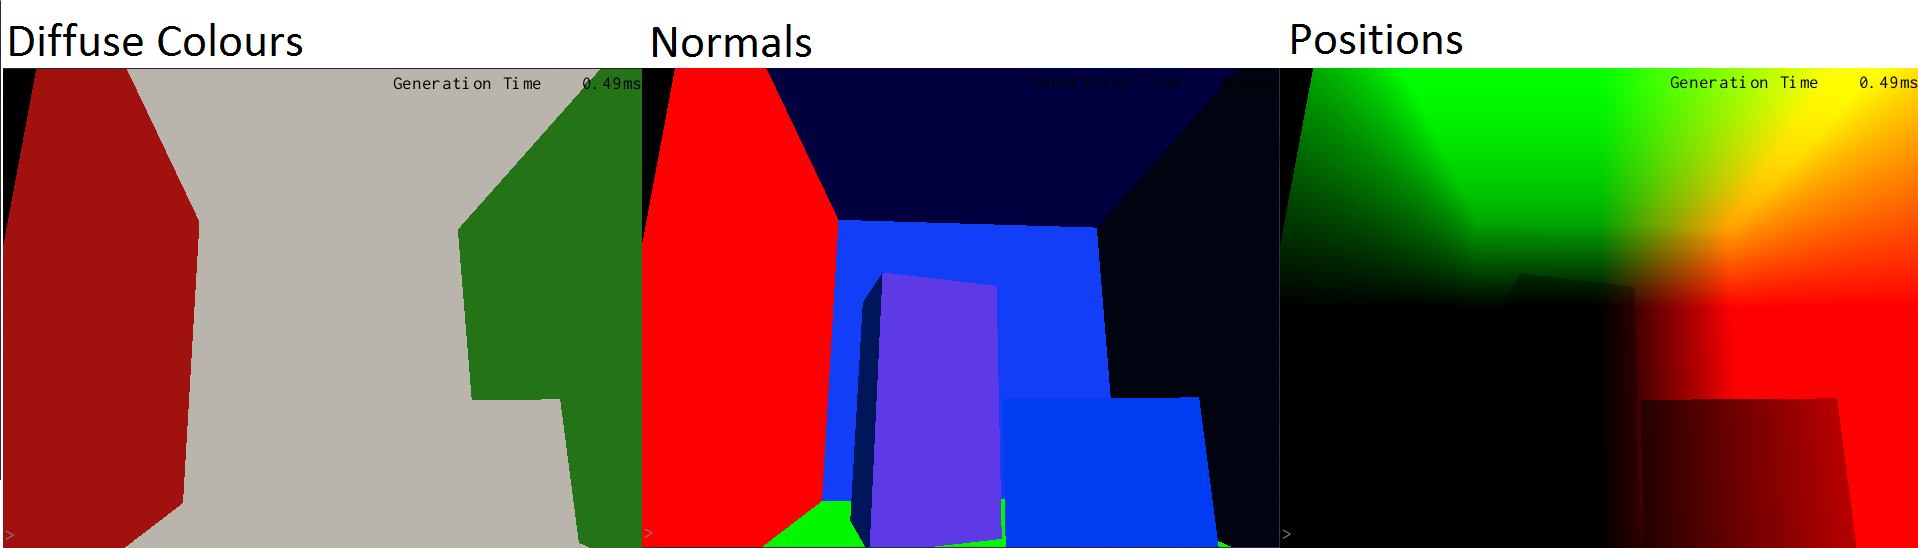
\includegraphics[width=1.0\textwidth]{img/def-rend/all}
    \caption{The contents of the G-buffer textures for the Cornell Box scene. There's no blue, since the eye direction is aligned along the negative Z-axis in view-space.}
    \label{fig-deferred}
\end{figure}

\subsubsection{Utilising the G-buffer}

When we have done the generation, we have a certain number of textures containing the geometric information for the scene on a per-fragment basis. We wish to use this data to do rendering calculations to produce our final scene. To do this we rasterise a single quad by an orthogonal projection, so that it fills the viewport exactly. In doing so, we have a 1:1 correspondence between our buffers and whatever target we're rendering to (be that another temporary offscreen buffer or the backbuffer.) We then sample data from whichever buffers we need to do our calculations, and use that data to calculate the desired shading. Listing \ref{list-deferred-use}, shows a deferred shader calculating lambertian lighting on a G-buffer.

\begin{lstlisting}[caption={Deferred Lambertian shader}\label{list-deferred-use},language=GLSL]
#version 330
in vec2 screenUV;

uniform sampler2D normals;
uniform sampler2D positions;
uniform sampler2D diff_colors;

uniform vec3 lPos;
uniform vec3 lInt;

out lambert;

main(void) {
	vec3 normal = normalize(texture(normals,screenUV));
	vec3 position = texture(position,screenUV);
	vec3 K_d = texture(diff_colors,screenUV);

	vec3 lV = normalize(lPos - position);
	
	lambert = K_d * lInt * dot(normal,lV);
}
\end{lstlisting}
To get the \verb?screenUV? vector we have a vertex attribute of 2 floats, that run between 0 and 1 along each axis.

If you ran this shader multiple times with additive blending enabled, every run would add a new light source to the render target, without needing to rerasterise the scene.

\subsubsection{Disadvantages}
While deferred rendering has its clear advantages in terms of running time, there are some things for which forward rendering has the edge. The primary one of these is the inability to do transparent materials. For instance, if the scene contained a refractive water layer, you'd be unable to write the normal data of this layer to the off-screen buffers, since it already has to contain the values for the materials under the water. A way to get around this is to do a forward render pass as the last step of the render pipeline, in which transparent objects are drawn with the uncleared depth buffer from the generation step. This would allow you to use the render target without the water (or other transparent surface) to look up offset values based on refraction index and normals of the surface.

Reflections can also cause problems, but they can be written directly to the G-buffer by the use of a stencil buffer and changes to the depth-test function. This, however, is only the case for G-buffers that do not have to be reconstructed from the depth buffer, whilst the method explained in \ref{section-reconstruction} has a few more caveats.

\subsection{The Deep G-buffer}
\label{section-deepbuffer}
When you start using the screen-space/G-buffer for more spatially conscious shading (such as radiosity or ambient occlusion,) pure single-layer G-buffers lack in apparent scene consistency. The traditional G-buffer simply does not contain anything beyond the top layer of geometry, and as such the same scene can seem visually inconsistent at two different angles. As an attempt to alleviate this shortcoming of deferred rendering, this thesis revolves around the use of a two layer deep G-buffer for global illumination approximations in screen-space. I will explain the technique as it is described in the paper \emph{Fast Global Illumination Approximations on Deep G-Buffers} by Michael Mara et al.\cite{deep-g-buffer}. What this method provides is a second layer of geometry, which means that shading stages has access to more geometric information about the scene, and thus is able to provide better and more visually consistent approximations of advanced effects.

The first thing we need to do to enable layered rendering, is to create array textures that contain the same number textures as the number of layers we wish to rasterise for our scene. Using array textures as render targets for an FBO works exactly like it does with with regular 2D textures, but obviously all texture have to have the same number of layers. The texture set up is also slightly different, since array textures are bound and initialised differently from flat textures in OpenGL. Listing \ref{list-deeptex} shows the OpenGL code to generate and initialise a 2-layer deep array texture.

\begin{lstlisting}[caption={Array texture initialisation for deferred rendering.}\label{list-deeptex},language=c++]
GLuint arrayTexture;

glGenTextures(1, &arrayTexture);
glBindTexture(GL_TEXTURE_2D_ARRAY,arrayTexture);

glTexParameteri(GL_TEXTURE_2D_ARRAY,GL_TEXTURE_MIN_FILTER,GL_NEAREST);
glTexParameteri(GL_TEXTURE_2D_ARRAY,GL_TEXTURE_MAG_FILTER,GL_NEAREST);
glTexParameteri(GL_TEXTURE_2D_ARRAY,GL_TEXTURE_WRAP_S,GL_CLAMP_TO_EDGE);
glTexParameteri(GL_TEXTURE_2D_ARRAY,GL_TEXTURE_WRAP_T,GL_CLAMP_TO_EDGE);

glTexImage3D(GL_TEXTURE_2D_ARRAY,0,GL_RGBA,width,height,2,0,GL_RGBA,GL_UNSIGNED_BYTE,0);
\end{lstlisting}

After we've tied our array textures to the FBO's colour attachments, we need to set up G-buffer generation such that it draws both layers of geometry to the texture. Figure \ref{fig-deep-buffer} shows the effect we wish to achieve, in which fragments that are occluded by the top layer of geometry are in stead written to the second layer of the G-buffer textures. In order to achieve this, we set up a geometry shader that emits all geometry directly and without modifications to both layers, as demonstrated in listing \ref{list-deepgeom}. Ultimately we do the test to determine whether or not to actually write the values in the fragment shader.

\begin{lstlisting}[caption={Geometry shader for 2-layer rendering.}\label{list-deepgeom},language=GLSL]
#version 330

layout(triangles) in;
layout(triangle_strip, max_vertices=6) out;

in vec3 outNormal[];
in vec4 outPos[];
in vec4 screenPos[];
in vec2 screenUV[];

out vec3 normalIn;
noperspective out vec2 screenUVFrag;
//noperspective because the screen UVs are linear in screen space.
out vec3 screenPosFrag;
flat out int layer;

void main() {
	layer = 0;
	gl_Layer = 0;
	for(int i = 0; i < 3; i++) {
		normalIn = outNormal[i];
		screenUVFrag = screenUV[i];
		screenPosFrag = vec3(screenPos[i]);
		EmitVertex();
	}
	EndPrimitive();
	
	layer = 1;
	gl_Layer = 1;
	for(int i = 0; i < 3; i++) {
		normalIn = outNormal[i];
		screenUVFrag = screenUV[i];
		screenPosFrag = vec3(screenPos[i]);
		gl_Position = outPos[i];
		EmitVertex();
	}
	EndPrimitive();
}
\end{lstlisting}

\begin{figure}[!ht]
  \centering
    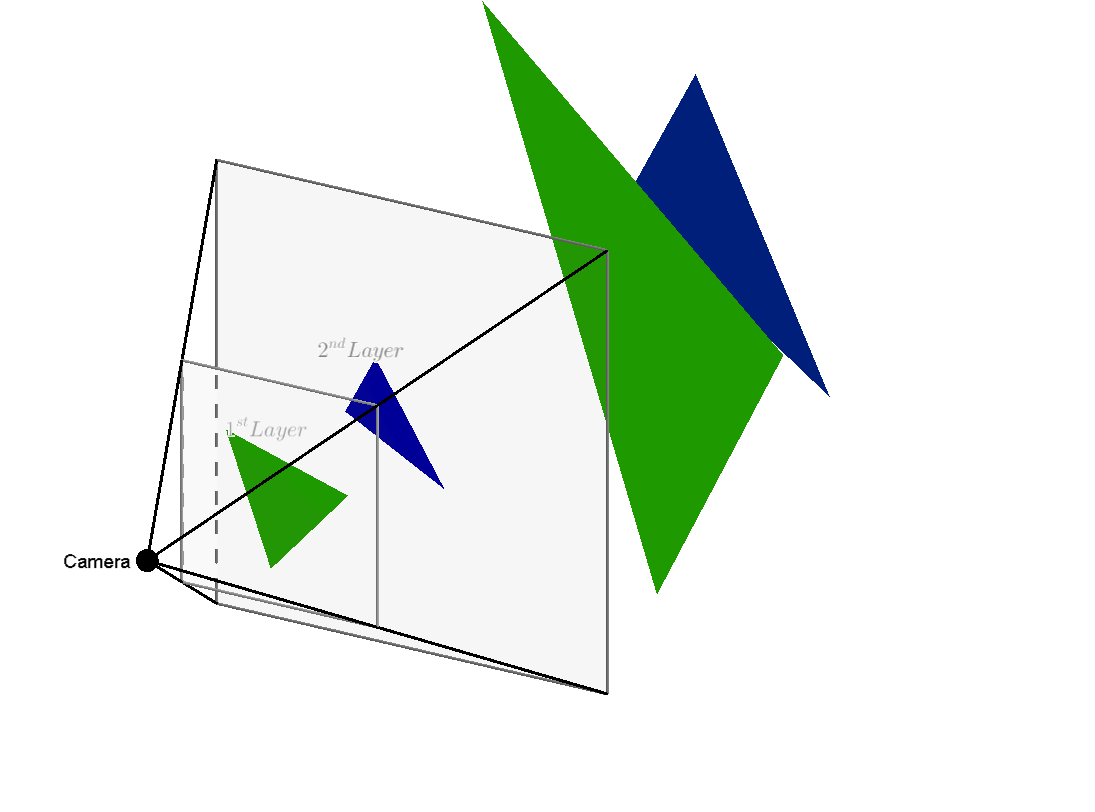
\includegraphics[width=0.8\textwidth]{img/2-layer}
    \caption{Illustration demonstrates the concept of a deep G-buffer. The green triangle is occluding the blue triangle. As a consequence, the blue one is written to the second layer of the G-buffer.}
    \label{fig-deep-buffer}
\end{figure}

Since the depth buffer is already making sure that the correct values are being written to the top layer of geometry, we can write values to layer 1 without doing any tests first. The second layer, however, is dependent upon whether or not geometry is occluded by the first layer. We can't use the currently bound depth-buffer to test this because it is actively being written to, and besides, there's no way of knowing what values might be written to it later (if we, for instance, determine that a piece of geometry does \emph{not} belong in the second layer, but another piece of geometry later overwrites it on the first layer.) As such, we need to buffer the depth buffer from the previous G-buffer generation, so that we can use it to predict whether or not a value belongs in the second layer. A naïve way to do this is to just use the previous run's depth buffer directly, and look up in its texture with the current run's screen UV-coordinates. This approach produces reasonable results, but at high generation times ($>20ms$) the secondary layer obviously "slags" when the camera moves around. This occurs because the shader is looking up "outdated" values. Another, more expensive option, is to rasterise geometry for both the current and previous frame, and use the previous frame's device coordinates to find the UVs to look up depth values. There's still some error related to the latter of the methods, but this is negligible compared to that of the former.

We also need to establish a minimal layer of separation between the two layers. Due to floating point imprecision, if we just look up the expected depth value of layer 1 and compare it to the Z value of the \verb=FragCoord=, we are going to Z-fighting artefacts in the second layer. The same effect causes shadow acne if you do not add a bias to a shadow map lookup. We set our separation in terms of fraction of the frustum depth. That is to say the space where 0 is the near-plane and 1 is the far-plane. This allows us to use the same layer of separation based on the definition of the projection planes. Choosing the right value to separate our two layers is a question of what parts of the scene we deem important. If we set it low enough, we can have back-facing geometry in the second layer, whereas high separation (or drawing with back-face culling) will cut off back-facing geometry to allow for deeper elements in the scene to appear in the second layer. Specifically how to set the value will vary depending on personal tastes and the scene you're working with. In this thesis we're working with a layer of separation that will draw back-facing geometry. To make the concept of depth consistent, we also linearise the depth values, since OpenGL packs depth values in a way that allows for more precision closer to the near-plane. To determine if a fragment is written to the second layer, we compare the calculated Z-coordinate with the Z-value read from the depth texture offset by our minimal layer of separation. If the calculated Z-coordinate is lower than the comparison value, we discard the fragment. The fragment shader for generating the 2-layer G-buffer can be seen in listing \ref{list-deepfrag}.

\begin{lstlisting}[caption={Fragment shader to generate the 2-layer G-buffer. No position is being written, which will be explained in section \ref{section-reconstruction}}\label{list-deepfrag},language=GLSL]
#version 330

in vec3 normalIn;
noperspective in vec2 screenUVFrag;
in vec3 screenPosFrag;
flat in int layer;

uniform sampler2DArray depth_texture;
uniform float near_plane;
uniform float far_plane;
uniform vec4 diff_color;
uniform vec4 spec_color;

layout(location=0) out vec3 normal;
layout(location=1) out vec4 diffColor;
layout(location=2) out vec4 specColor;

float linearDepth(in float depth){
	return (2.0 * near_plane) / (far_plane + near_plane - depth * (far_plane - near_plane));
}

void main() {

	switch(layer) {
		case 0:
			//Write data to buffer
			break;
		case 1:
			if(linearDepth(gl_FragCoord.z) <= linearDepth(texture(depth_texture,vec3(screenUVFrag,0)).r) + 0.01f)
				discard;
			else {
				//Write data to buffer
			}
			break;
	}

}
\end{lstlisting}

The comparison depth texture is a \verb=sampler2DArray= since it's 2-layered. We only use the first layer, however, since that is all we need to determine if a fragment belongs in layer if the output buffer. We also use \verb=sampler2DArray=s to sample when we do the deferred shading. Utilising the deep G-buffer is similar to the way we utilise a flat G-buffer, except our input textures are texture arrays. When we use it for our global illumination approximations we sample both layers at the same screen-space taps. If we wish to buffer information from a filter for both layers, we use a geometry shader to commit our full-screen quad twice, once for each layer.

\subsection{Scene Reconstruction}
\label{section-reconstruction}
The total memory cost of a naïvely implemented, 1-layer G-buffer with just normals, positions and material properties would, at the very least, be 128 bits, or 16 bytes, of information buffered per fragment. That is with 16-bit precision normals and positions ($16 bits * 3 channels * 2 buffers = 96 bits$, and a regular RGBA 8-bit precision diffuse reflectance (32 bits.) With 32-bit precision on positions, which would give noticeably better results, the total would end up being 176 bits, or 22 bytes, per fragment. For a 1080p (\verb=1920*1080=) buffer, the total memory usage for the G-buffer alone would end up at just under 44MB. Keep in mind that this is for the bare essentials, without any additional G-buffer related data like radiosity, SSAO, specular reflectance, shininess etc. It would definitely be possible to work around this memory usage by saving in other areas (textures, models;) even on a system with as little as 512MB of VRAM. Where the need to search for alternate solutions comes in, is with the use of a deep G-buffer. With a deep G-buffer all assumed VRAM useage for the G-buffer has to be multiplied by 2, meaning that our original 44MB becomes 87MB, and for every additional 32-bit buffer we use we have to add another 16MB (8MB for each layer.) Additionally, we need the previous frame's depth buffer to be able to tell whether or not a fragment belongs in the second layer of the G-buffer, which adds another 64 bits (8 bytes) per fragment (One for the current and one for the previous frame.) Luckily, there's a way to trade performance for less VRAM usage, both for positions and normals, by reconstructing information from the least amount of vital information. I will explain both of these here, but the product of this thesis only implements the reconstruction of positions.

\subsubsection{Reconstructing Positions}
In order to reconstruct positions, all we really need to buffer is the depth. In the reconstruction step, we can use the UV-coordinates of the full-screen quad to find the normalized device coordinates, and since we know the projection matrix by which the scene was projected, we can find the view-space coordinates of the fragment. Using the depth buffer also means we save a write operation when we generate the G-buffer, since we need a depth-buffer active for depth-testing regardless of whether or not we reserve its results for later. This offsets some of the cost of the reconstruction later. We tie a 2-layer array texture with internal format \verb=GL_DEPTH_COMPONENT32= to the depth attachment on the G-buffer generation FBO. The texture generation is the same as is shown in listing \ref{list-deeptex}, except the internal format is a 32-bit depth component. We then tie it to the depth attachment of the FBO like shown in listing \ref{list-depthFBO}. Note, that the depth attachment will have to be swapped around between frames due to its usage in predicting the contents of the deep layer.

\begin{lstlisting}[caption={Tying the depth texture to the depth component of the FBO}\label{list-depthFBO},language=c++]
GLuint FBO;
glGenFramebuffers(1,&FBO);
glBindFramebuffer(GL_DRAW_FRAMEBUFFER, FBO);
glFramebufferTexture(GL_DRAW_FRAMEBUFFER,GL_DEPTH_ATTACHMENT,depth_texture,0);
//Tie other textures to their relevant colour attachments.
\end{lstlisting}

With the depth information (as a number between 0 and 1) and screen-space UV-coordinates available in our reconstruction stage, we can find the normalised device coordinates for a fragment ($\mathbf{v} = 2((\mathbf{UV}_x,\mathbf{UV}_y,depth,0) - 0.5) + (0,0,0,1)$,) and using the inverse of the projection matrix used to project the scene in the generation stage, we can unproject these into coordinates with the right proportions in relation to each other, due to the following relationship:

$$\underline{\underline{M}}^{-1}\underline{\underline{M}} = \underline{\underline{I}}$$
$$\underline{\underline{M}}^{-1}\underline{\underline{M}} \mathbf{v} = \mathbf{v}$$
$$\underline{\underline{P}}^{-1}\underline{\underline{P}}\underline{\underline{V}}\underline{\underline{M}}\mathbf{v} = \underline{\underline{V}}\underline{\underline{M}}\mathbf{v}$$

To get the true view-space coordinates we ultimately do W-division: $\mathbf{X} = \frac{\mathbf{v}_{xyz}}{\mathbf{v}_w}$. In doing this, we save 64 bits per layer per fragment, or a total of 128 bits of storage per fragment for positions, assuming a 96-bit position buffer. We also save at least two memory taps, due to the GPU needing more memory reads to retrieve a 96-bit texel than a 32-bit one.

A major disadvantage with reconstructing the scene from a depth-buffer, is that we can no longer do reflections using deferred rendering. This is because the view matrix is different for parts of the scene that are reflected, and as such the entire depth buffer cannot be reconstructed in a single go. This can be fixed, however, by either doing ray-traced reflections in screen-space in a later filtering stage or using stencil buffers to which you draw the reflective parts of the scene to only reconstruct and shade parts of the scene for which a given MVP-matrix is valid. This method does add overhead both in terms of more state changes, more shading computations and more memory usage.

\subsubsection{Reconstructing Normals}
In regards to normals, we can utilise the fact that we know its length in order to reconstruct the third of its coordinates from the two others by simply doing $\pm Z = \sqrt{X^2 + Y^2 - 1}$. While this in and of itself is not very complicated, and most modern GPUs do the calculation $\frac{1}{\sqrt{X}}$ in a single cycle, meaning it wouldn't necessarily be very expensive, the issue arises in determining the sign of the third coordinate. Since central projection, which is what I use in the product of this thesis, allows for geometry facing away from the near plane to be rasterised, and X and Y coordinates are independent of screen-space positions, we would need to somehow buffer the sign of Z if we wanted to save only two coordinates for every normal. One way to do this would be to use an available 8-bit channel in one of the colour buffers, which both have an alpha channel available (although we use the $\rho_s$ alpha to store shininess.) This, however, requires us to do an additional texture tap whenever we want to use our normals. A better solution would be to sacrifice precision in either the Y or X coordinate by encoding the sign of Z into the least significant bit of the mantissa of either. The problem with this method is that it requires the use of integer operations, which are not widely supported by GPUs yet, and there's some performance hit involved in doing so.
I originally used \verb$R11_G11_B10$ float textures to buffer normals, which does not have a sign on its mantissa. These were encoded by dividing by 2 and adding a half. However, the lack of precision in this format (causing inconsistent lighting between angle changes,) and the hardware related costs of interpreting them for use in a shader meant that I ultimately settled on the traditional \verb$RGB16F$ format.

\section{Omnidirectional Shadowmapping}
While we we assume for radiosity that the visibility term is equal to 1, and aren't doing any occlusion testing on the hemisphere samples, we wish to do occlusion testing for the diffuse reflectance of radiance directly from the light source. We will use a simple Lambertian shader for our initial radiosity result, multiplied by a visibility term, which we will find based on a look up into a shadow map. Lambertian shading calculated diffuse radiance from a surface like so:

$$L_e(\mathbf{x}) = \frac{1}{atten}\frac{\rho_d}{\pi} I_l cos(\theta) V(\mathbf{l} \rightarrow \mathbf{x})$$

Where $atten$ is the attenuation of the light (for directional lights this is 1,) $\rho_d$ is the diffuse reflectance, which is a vector with values between 0 and 1, $I_l$ is the intensity of the light source, $\theta$ is the angle between the normalised vector from our point to the light source and $V()$ is the visibility term.

In order to evaluate the visibility term we will employ a shadow-map. However, since we want to support point lights and work regardless of what and how many elements are in the scene, this is slightly more tricky than simply implementing a simple one-texture shadow-map that contains normalized clip-space coordinates. To accomplish full coverage around our point light, we need to use something called an omni-directional shadow map. There are several ways to achieve this, but the simplest and most precise is one in which you render your scene unto a cube-map and buffer the clip-space distance from the light source to a given fragment. The process of rendering to a cube map is very similar to that of rendering the deep G-buffer, in that the cube-map is essentially just a 6-layered array texture in which each layer represents a face on the cube. The process of preparing a cube map as a render target is demonstrated in listing \ref{list-cube-tex}. Notice, we only tie a render target to the depth buffer, since that is all we need.

\begin{lstlisting}[caption={Setting up the cube map for rendering}\label{list-cube-tex},language=c++]
//Texture and FBO generation
glGenTextures(1, &shadowDepth);
glGenFramebuffers(1, &shadowFBO);

glBindTexture(GL_TEXTURE_CUBE_MAP, shadowDepth);
//Set parameters for texture
glTexParameteri(GL_TEXTURE_CUBE_MAP, GL_TEXTURE_WRAP_S, GL_CLAMP_TO_EDGE);
glTexParameteri(GL_TEXTURE_CUBE_MAP, GL_TEXTURE_WRAP_T, GL_CLAMP_TO_EDGE);
glTexParameteri(GL_TEXTURE_CUBE_MAP, GL_TEXTURE_WRAP_R, GL_CLAMP_TO_EDGE);
glTexParameteri(GL_TEXTURE_CUBE_MAP, GL_TEXTURE_MAG_FILTER, GL_LINEAR);
glTexParameteri(GL_TEXTURE_CUBE_MAP, GL_TEXTURE_MIN_FILTER, GL_LINEAR);
//For each layer in the cube-map we initialise its contents
for(GLuint i = 0; i < 6; i++) {
	glTexImage2D(GL_TEXTURE_CUBE_MAP_POSITIVE_X + i, 0, GL_DEPTH_COMPONENT32F, SHADOW_WIDTH, SHADOW_HEIGHT, 0, GL_DEPTH_COMPONENT, GL_UNSIGNED_BYTE, nullptr);
	
glBindFramebuffer(GL_DRAW_FRAMEBUFFER,shadowFBO);
//Tie the cube map texture to the depth attachment of the FBO.
glFramebufferTexture(GL_DRAW_FRAMEBUFFER,GL_DEPTH_ATTACHMENT,shadowDepth,0);
\end{lstlisting}

We use the same projection matrix for all layers, which is a central projection with a $\frac{\pi}{2}$ field of view. The FOV has to be exactly that, since that means the frustums for all sides of the cube line up such that when geometry is split between two sides, it will line up on the cube. We also set the view matrices such that they line up in accordance with \cite{cubetex}. We then draw the length of the position vector divided by the far plane to the depth buffer. An important note here is to \emph{not} let the pipeline interpolate the depth between vertices, but calculate it in the vertex shader based on the interpolated position vector, since the depth does not change linearly across an edge. We use the length of the position vector since it easens our look-up when we evaluate the visibility term. The length of the vector from a point to the light source can then be used to determine occlusion. If we used the projected fragment depth, we'd first have to figure out which coordinate of the light vector to use for our comparison.

Since the view matrices used to generate the shadow map are in world space, and we calculate data to be in screen-space, when we do the lighting calculations we have to also remember to multiply our regenerated position vector by the inverse view matrix originally used to rasterise the scene. This way we obtain world-coordinates, which are needed for the shadow map look up.

One of the major advantages of using a cubemap texture for our omni-directional shadowmap is that you access cubemaps by looking up a direction in stead of a UV-coordinate. What this means is that we can use the world-space normalized light vector to find the value we need to compare by to determine visibility. We then simply take the length of the light vector, divide it by the far plane, and if it is less than or equal to the value in the shadowmap, the fragment is \emph{not} occluded. We subtract a very small bias from the light vector length to get rid of shadow acne.

\section{Radiosity}
\label{section-radiosity}
Radiosity is a method to determine light transfer between purely diffuse surfaces. That is to say it covers only the case in which incident radiance at a surface is distributed equally in all directions, and the amount of energy that is transferred between surfaces by this method. We will take a point of departure in the rendering equation, explain the predominant "slow" radiosity method of dividing the scene into patches and explain the screen-space approximation used in the final product.

\subsection{The Rendering Equation}
\label{section-renderingequation}
The rendering equation sets up the radiance from a point towards another point as the sum of its emitted radiance and an integral over the hemisphere to gather radiant exitance based on incident radiance, outgoing direction, incoming direction and the wavelength of light. It can be denoted in multiple ways, here we will write it like this: Figure \ref{fig-rendering-eq} denotes what symbols represent spatially.

$$L(\mathbf{x} \rightarrow \overline{\omega_0},\lambda) = L_e(x \rightarrow \omega_o,\lambda) + \int_\Omega F_r(\mathbf{x},\overline{\omega_i},\overline{\omega_0},\lambda) I_i(\omega_i \rightarrow \mathbf{x}) \cos(\theta) d\omega_i$$

\begin{figure}[!ht]
  \centering
    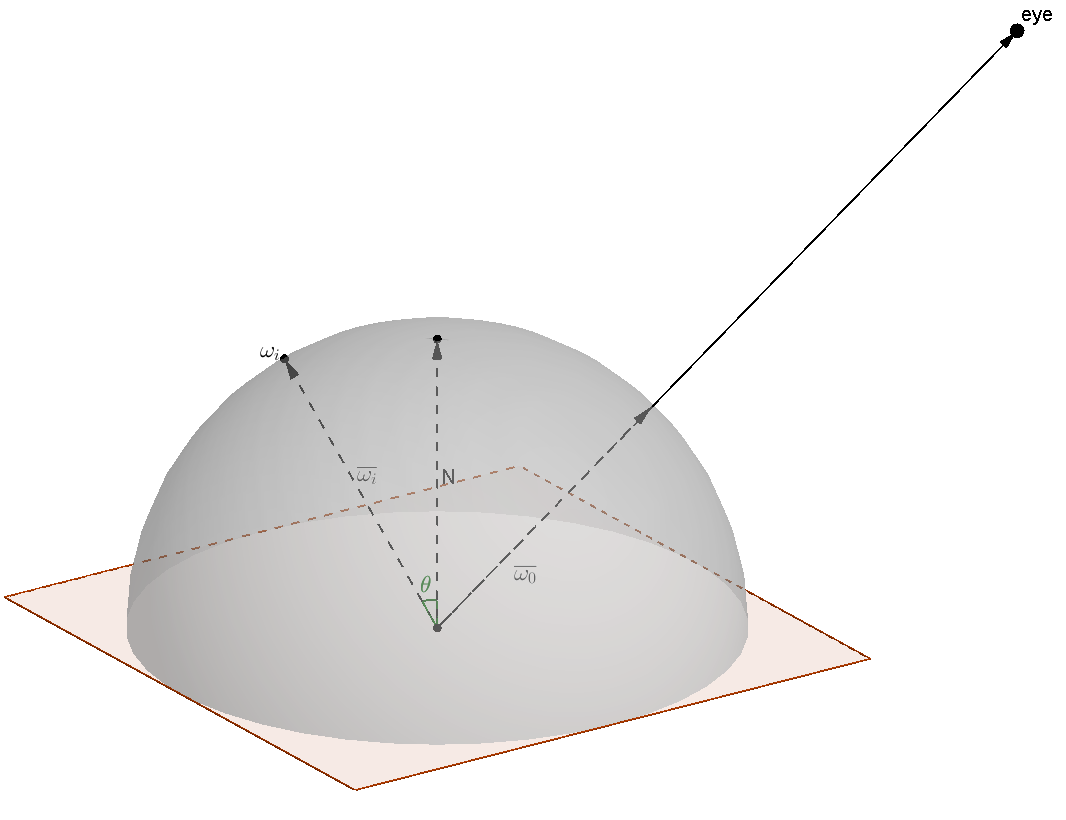
\includegraphics[width=0.8\textwidth]{img/rendering-eq}
    \caption{A visual representation of the rendering equation, with symbolic values annotated.}
    \label{fig-rendering-eq}
\end{figure}

We integrate over the hemisphere around the normal of the point, to gather radiance reflected towards our view position.\\
$\mathbf{x}$ represents the point in space we're currently investigating.\\
$\overline{\omega_0}$ is the normalized vector from $\mathbf{x}$ towards the point to which radiance is emitted (or the view point.)\\
$\lambda$ is the wavelength of the light.\\
$\Omega$ is the surface of the hemisphere.\\
$\omega_i$ refers to the infinitessimal solid angle on the hemisphere.
$\overline{\omega_i}$ is the direction from $\mathbf{x}$ to $\omega_i$.\\
$\theta$ is the angle between the normal of $\mathbf{x}$ and $\overline{\omega_i}$\\

$L_e()$ is emitted radiance, which is not part of the scope of this thesis. For the purpose of radiosity, the interesting part is the integral. One way to think of it is that it's an integral of a function $I(\omega)$ whose function values are the irradiance incoming from are $\omega$ which runs over a known surface (the hemisphere.) $F_r$ is the Bi-Ray Distribution Function, which is a function that varies depending on the material properties of the point of incidence. It produces a factor by which to multiply the irradiance from $\omega_i$, $I_i$, based on $\overline{\omega_i}$, $\overline{\omega_0}$ and $\lambda$. Like mentioned radiosity is only concerned with the case of perfectly diffuse surfaces, meaning that total irradiance is distributed equally across the hemisphere, regardless of incoming direction. As such, the BRDF is completely independent of the direction of irradiance (as long as it is on the hemisphere) and how it relates to the view direction. It is, however, dependent upon $\lambda$, since the material will absorb light of certain wavelengths based on its colour. The BRDF of a perfectly diffuse surface is therefore simply $K_d$ or $\frac{\rho_d}{\pi}$.

For diffuse light transfer we will assume a perfectly closed system, in which all surfaces are perfectly diffuse. This will allow us to write up a rendering equation for radiosity:

$$L(\mathbf{\mathbf{X}} \rightarrow \mathbf{e}) = B(\mathbf{X}) = \int_\Omega \frac{\rho_d}{\pi} B(\mathbf{Y}) \cos(\theta) d\omega_i$$

What this means is that radiance received for our eye point, $\mathbf{e}$, from point $\mathbf{X}$, is obtained by integrating radiosities for all points visible from point $\mathbf{X}$ across the hemisphere.. Point $\mathbf{Y}$ denotes the point in direction $\overline{\omega_i}$ from $\mathbf{X}$. A simple way to obtain multiple bounces from a naive implementation of this equation, would be to consider it a recursive function. That is to say, for every $\omega_i$, consider its corresponding $\mathbf{Y}$ the subject of another radiosity gather, in which the eye point, $\mathbf{e}$ is now the original $\mathbf{X}$ and $\mathbf{X}$ is now the original $\mathbf{Y}$. For every layer of recursion added to this method, we'd get another bounce. However, running such an algorithm for every pixel in a ray tracer would be prohibitively expensive, even with decent sampling optimisations. The complexity of such a recursive method would be $O(p \cdot b^n)$, where $p$ is the total number of pixels sampled, $b$ is the number of bounces and $m$ is the number of samples used to approximate the integral. As such, other methods are employed to approximate this effect in a more reasonable time.

\subsection{The Patch Method}
The patch method is the most common way to solve the radiosity problem in "slow" time (as opposed to real-time.) In it, you divide your scene into discrete patches, each of which has an amount of energy attached to it, which is distributed as radiosity to other patches in the scene. It is usually used as a pre-baking method, in which radiosity is done for diffuse surfaces and mapped unto the scene when it is ray-traced, or, for real-time applications, rasterised. It has the distinct disadvantage for the latter application, since the generation time does not allow for the radiosity map to be regenerated on-the-fly (at least not on current generation hardware.) Therefore radiosity by the patch method will typically be done only once for real-time applications, which means that radiosity for scenes with dynamic lighting, shadows and geometry will not change over time. The product of this thesis does not implement a patch method, but as was mentioned it is the most common method employed, and will provide a good contrast to the screen-space method explained in \ref{section-ssradiosity}.

With the patch method, we wish to approximate the integral over the hemisphere with discrete patches in space. A discretisation of the radiosity equation from \ref{section-renderingequation}, in which we loop over all other patches in the scene, to gather up all radiosity for a single patch, looks like this:

$$B(X) = \sum_{i=0}^{n} \frac{\rho_d}{\pi} \int_{t_0} \int_{t_i} B(i) \cos(\theta_i) V(x \rightarrow y) dt_i dt_0$$
$n$ is the number of patches in the scene.\\
$t_0$ is the patch for which we are currently gathering radiosity.\\
$t_i$ is the $i^{th}$ patch.\\
$V()$ is the visibility term, which is either a value of 1 or 0 depending on whether or not the infinitesimal point $y$ on $t_i$ is visible from the infinitesimal point $x$ on $t_0$.

We integrate over our patch, and for every infinitesimal point on it, we integrate over the patch from which we are currently gathering radiosity. Of course, these internal integrals are still not discretised, but to achieve simple computations we replace them with something called the form factor. What we essentially want is to determine the area which $t_i$ covers on the hemisphere of $t_0$. We also include $cos(\theta_i) V(x \rightarrow y)$ in this factor, so that all the geometry terms are included. We rewrite $cos(\theta_i) V(x \rightarrow y)dt_i dt_0$ to:\cite{radiosity}

$$F_{0i} = \frac{1}{A_0} \int_{A_0} \int_{A_i} \frac{cos(\theta_i) cos(\theta_0)}{\pi r^2}  V(x \rightarrow y) dA_i dA_0$$

Where $r$ is the distance from $t_0$ to $t_i$. We estimate this numerically by simply replacing $dA_i d_A0$ by the areas of the two patches ($A_i$ is eliminated because of the division):

$$F_{0i} \approx A_i \frac{cos(\theta_i) cos(\theta_0)}{\pi r^2}  V(x \rightarrow y)$$

The equation is currently written from the point of view of the gatherer; that is to say we calculate radiosity received based on an integral over the hemisphere of the gatherer. For the patch method it makes more sense to consider the point of the view of the distributor, seeing as once the distributor's energy has been exhausted, we can set its total energy to zero, since it has all been expended. Making such a change is fairly straight forward in code, seeing as the form factor and visibility terms merely have to be swapped around. If we consider $\mathbf{X}$ our distributor, we loop over all other patches, and based on the form factor, visibility term and radiosity of $\mathbf{X}$, we add to the radiosity of these patches. This type of buffered method does not allow us to do multiple bounces sequentially, as the distribution changes the radiosity levels of other patches. However, we can always make sure to distribute for the most significant patch at any given time, by sorting the list of patches by highest radiosity. Listing \ref{list-patchDist} shows how a single patch distributes its energy.

\begin{lstlisting}[caption={A single patch distributing its energy to other patches in the scene.}\label{list-patchDist},language=c++]
List<Patch*> patches;
Patch currentPatch = pathces[0];
for(int i = 1; i < patches.length; i++) {
    patches[i]->radiosity += patches[i]->K_d * currentPatch->radiosity
    * max(dot(currentPatch->normal,normalize(pathces[i]->pos - currentPatch->pos)),0);
    * visFactor(currentPatch,&patches[i])
    * formFactor(currentPatch,&patches[i]);
}
currentPatch.radiosity = 0;
\end{lstlisting}

There are multiple ways to evaluate the visibility factor. One is to trace a ray through the scene along the vector between the two patches and test for collisions. Another one, which also easens the evaluation of the form factor, is to project other patches unto a cube around the distributor patch using a rasteriser pipeline with depth testing (aka the hemicube method.)

\subsection{Screen-Space Methodology}
\label{section-ssradiosity}
The method we wish to deploy is one that takes advantage of the deep G-buffer specified in \ref{section-deepbuffer} to do real-time radiosity calculations. As such, we need a screen-space approximation. In this section I will explain a way to achieve such an approximation by sampling both layers of the G-buffer according to a parametrised curve using quasi-Monte Carlo sampling, and how to consider the rendering equation for radiosity to approximate the integral over the hemisphere.

\subsubsection{Monte Carlo Integration}
Monte Carlo sampling is a way to approximate integrals by doing random samples from the total of function values. In order to explain it, we will take a point of departure in Riemann Integration. The idea behind the Riemann Integral is that in order to find the integral of a given function, you sum up the function values of incrementing $x$-values and multiplying by the change in $x$.

$$\mathbf{F}(x) = \sum_{i = 0}^{n}f(x\frac{i}{n}) \Delta x$$

Where $n$ is the number of $x$-values used to find the integral and $\Delta x$ is the width of each segment, or $\frac{x}{n}$. If we let $n$ tend towards $\infty$ we get a continuous integral.

For our purposes, however, we do not know a function describing the distribution of irradiance on the hemisphere, but we are able to sample our screen-space for function values. Monte Carlo integration is a way to find the integral of an unknown function, by sampling function values at random, and giving them all equal weight. In a sense, it is a return to the base of the Riemann Integral. We wish to use Monte Carlo integration to solve the following integral:

$$L(\mathbf{X} \rightarrow \mathbf{e}) = B(\mathbf{X}) = \int_\Omega \frac{\rho_d}{\pi} B(\mathbf{Y}) \cos(\theta) d\omega_i$$

Ideally, to approximate this integral we would trace rays in cosine-weighted random directions around the normal of $\mathbf{X}$, and weigh each of them based on their proportion of the hemisphere. We write up the summation like so:

$$B(\mathbf{X}) = \sum_{i=0}^{n} \frac{\rho_d}{\pi} B(\mathbf{Y}(\omega_i)) \cos(\theta) \Delta \omega_i$$

Here $\omega$ can be considered an array of length $n$ of properly distributed, random directions. The point $\mathbf{Y(\omega_i})$ is the point resulting from ray-tracing in direction $\omega_i$. If we let the size of the array, $n$, tend towards infinity, the result becomes accurate thanks to the Law of Large Numbers. Since we know that the total area of the hemisphere is $2\pi$, the sum of all infinitesimal angles, $d\omega_i$, is $2\pi$, and we assume that for every ray we trace, the result we get from the scene will cover an equal part of the hemisphere, we get the following sum:

$$B(\mathbf{X}) = \frac{2\pi}{n} \frac{\rho_d}{\pi} \sum_{i=0}^{n} B(\mathbf{Y}[\omega_i]) \cos(\theta)$$

Of course, a problem occurs since we're working in screen-space, and that is that we do not have access to a ray-tracer, and only geometry in the viewing frustum is immediately available to us. The former will be alleviated by the use of a Quasi-Monte Carlo sampling method explained in the next section. The latter is an inherent problem with screen-space methods, and while remedies exist in the form of other non-screen-space methods, this problem will not be solved as part of this thesis.

\subsubsection{Quasi-Monte Carlo}
Since Monte Carlo approximations rely on completely random samples of function values, with a low number of samples the relative chance of errors is high. This occurs because true randomisation (or even pseudo-randomisation) only guarantees tendency towards the result for a high number of samples (The Law of Large Numbers.) For real-time applications we're only going to have time for a limited number of texture taps per pixel per frame drawn. As such, we need a sampling strategy that distributes our chosen sampling points to cover as much space as possible, while also maintaining some randomisation to avoid structural bias. Thus, we want a function to distribute our sample point evenly in screen-space around our gather point under the assumption that this will give us the most even distribution of points on our hemisphere. We also want it to be distributed around the point for which we are gathering, which means we are looking for something to offset our sample taps.

To achieve these goals we will use a tap pattern that runs along a parametrised spiral, with every tap spaced evenly out along the spiral. We will start by looking at the parametrisation of a spiral, and how the different parameters for it affect its form. The parametric curve of a spiral in its simplest form is defined as:

$$\mathbf{v}(t) = t \begin{pmatrix}\cos(t) \\ \sin(t) \end{pmatrix}$$

While the curve for this function will produce a spiral, it doesn't allow much control of its form, and the arms of the spiral will be increasingly distant for larger values of $t$. We want fairly evenly distributed points in screen-space, with a way to randomise our spiral, control its radius and the number of turns it does within this radius. To do this we employ the following parametrisation:\cite{deep-g-buffer}

$$\sigma = t + \frac{\psi}{tau} $$
$$\theta = 2\pi\sigma\tau + \phi $$
$$\overline{u} = \begin{pmatrix}\cos(\theta) \\ \sin(\theta) \end{pmatrix} $$
$$h = R \sigma $$
$$\mathbf{v} = h \overline{u}$$
$$0 < t < 1, 0 < \phi < 2\pi, 0 < \psi < 1$$

This gives us a number of parameters to work with. $R$ is the radius of our spiral, when $t$ is 1, the length of $\mathbf{v}=R$. $\tau$ is the number of spiral turns are inside the spiral before it reaches $t = 1$, $\phi$ and $\psi$ are used to allow for some randomisation of the spiral; $\phi$ is an angle by which we rotate the entire spiral (randomising this to be unique for each fragment will allow us to trade structural noise for more random noise.) $\psi$ allows us to offset the start of the spiral up to one turn. Figure \ref{fig-spiralparam} demonstrates the spiral and how the parameters change its form.

\begin{figure}[!ht]
\begin{tabular} {| l | c | c | c | c |}
\hline
& 

\includegraphics[scale=0.2,trim={10cm 4.65cm 11.3cm 3.0cm},clip]{img/spiral/1turn}
&

\includegraphics[scale=0.2,trim={10cm 4.65cm 11.3cm 3.0cm},clip]{img/spiral/5turns}
&

\includegraphics[scale=0.2,trim={10cm 4.65cm 11.3cm 3.0cm},clip]{img/spiral/5internaloffset}
&

\includegraphics[scale=0.2,trim={10cm 4.65cm 11.3cm 3.0cm},clip]{img/spiral/pioffset}
\\
\hline
R (Radius) & $5$ & $5$ & $5$ & $5$ \\
\hline
$\tau$ (Spiral Turns) & $1$ & $5$ & $1$ & $1$ \\
\hline
$\phi$ (Rotation) & $0$ & $0$ & $0$ & $\pi$ \\
\hline
$\psi$ ($t$ Offset) & $0$ & $0$ & $0.5$ & $0$ \\
\hline
\end{tabular}
\caption{Demonstrates the consequence of different parameters for the spiral curve.}
\label{fig-spiralparam}
\end{figure}

We sample along the spiral by incrementing $t$ discretely from 0 to 1 given a certain number of samples. To achieve this we replace the form of $\theta$ by $\theta_i = \frac{i + \frac{\psi}{\tau}}{n}$ where $n$ is the number of samples we do. We end up with an algorithm that sums up irradiance like so:

$$\mathbf{p_i} = \mathbf{x} + \mathbf{v_i}$$
$$\overline{\omega_i} = | reconstruct(\mathbf{p_i}) - \mathbf{X} |$$
$$B(\mathbf{x}) = K_d \frac{2\pi}{m} \sum_{i = 0}^{n} B(\mathbf{p_i}) (\overline{n_X} \cdot \overline{\omega_i})$$

Where $X$ is the spatial point reconstructed from the screen-space tap $\mathbf{x}$ (our current gathering point,) $reconstruct()$ is a function that reconstructs the spatial point from the screen-space tap $\mathbf{p_i}$ and $m$ is the number of "accepted" sample taps. We discard all sample taps that are not on the hemisphere of $\mathbf{X}$, and the ones which extend beyond screen-space.

We need one final piece, and that is to determine the total number of spiral turns. For that we use the array defined in \cite{deep-g-buffer}. It is important that we fit the number of spiral turns to the number of sample taps, since not doing so can cause the taps to become "synched" from one turn to the next, meaning the spread is minimised. We tap both layers of the G-buffer at the same sample point positions in screen-space.

The final result of this method appears grainy as seen in figure \ref{fig-noise}, since we have traded off structural bias for more randomised noise. To alleviate this we will applya gaussian filter over the radiosity result. This filter is described in section \ref{section-gauss}.

\begin{figure}[!ht]
  	\centering
  	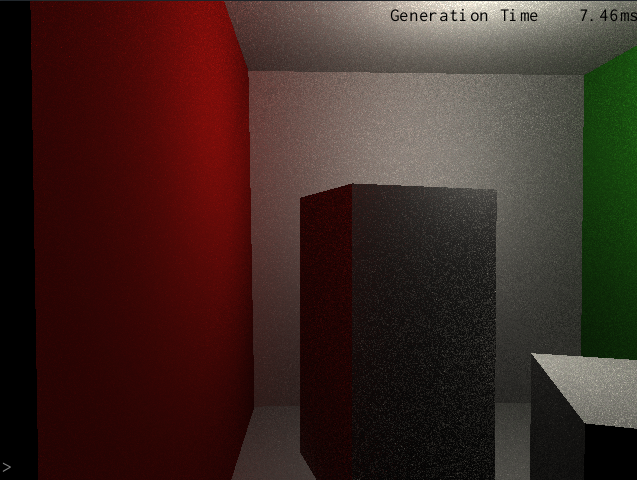
\includegraphics[width=0.8\textwidth]{img/noise}
    \caption{Unfiltered Radiosity result showing high level of random noise}
    \label{fig-noise}
\end{figure}

\section{SSAO}
SSAO or Screen-Space Ambient Occlusion is a way to evaluate the occlusion of ambient light for a given fragment, based on information available in the G-buffer. We use the alchemy AO method for this purpose:\cite{VV11AlchemyAO}

$$AO(\mathbf{X}) \approx max \left( 0 , 1 - \frac{2 \sigma}{s} \sum_{i = 1}^{s} \frac{max(0,\overline{v_i} \cdot \overline{n} + \mathbf{X_z} \beta)}{\mathbf{v}_i \cdot \mathbf{v}_i + \epsilon} \right) ^K$$

This function has a lower value the more geometry "covers" its hemisphere. The parameters to it are as follows:
$s$ is the number of samples.
$\sigma$ controls magnitude. The higher it is, the less it takes for geometry to count towards the obscurance of $\mathbf{X}$.
$\beta$ is used to reduce self-shadowing, but leaving it too high can cause lack of contributions.

We divide by the dot product of the $\mathbf{v}_i$ vector by itself in order to get some scaling with the size of the scene.

\section{Filtering}
The spiral for each individual pixel can be rotated by any value within $[0;2\pi]$, and only does $20\pm10$ samples per buffer layer, within a radius that spans tens of thousands of pixels. As such, there's a high amount of high-level noise, resulting in a grainy image with potentially big contrasts from pixel to pixel. Therefore, we need a filtering method which will level out the radiosity and AO to more smooth results across surfaces. To this end we will employ a traditional gaussian blur filter, with some modifications to improve on running time and avoid surfaces "bleeding" in to each other.

\subsection{Gaussian Filtering}
\label{section-gauss}
We employ a filter by looping through all pixels in our buffer, and for each pixel we wish to even its intensity out with its immediate neighbours. We do this in a radius around our center pixel, which we will denote by $R$. We denote our center pixel (that is to say the pixel for which we are currently applying the filter) by $P_c$ and the pixel at position $(x,y)$ in relation to $P_c$ as $P(x,y)$.
The Gaussian Filter is a filtering method that aims to average out neighbouring pixels according to their distances to each other as an argument to the Gaussian Function, also known as the bell curve or the normal distribution. In general terms, the Gaussian Function, $G(x)$ is defined as follows,

$$G(x) = \frac{1}{\sigma \sqrt{2\pi}} e ^ {-\frac{(x - \mu)^2}{2\sigma^2}}$$

In which $\sigma$ denotes the standard deviation and $\mu$ the mean. In the traditional normal distribution with $\sigma = 1$ and $\mu = 0$, $68\%$ of the area under the graph of the function will be within the interval $[-1;1]$. A plot of this function is seen in figure \ref{fig-gauss}.

\begin{figure}[!ht]
  	\centering
  	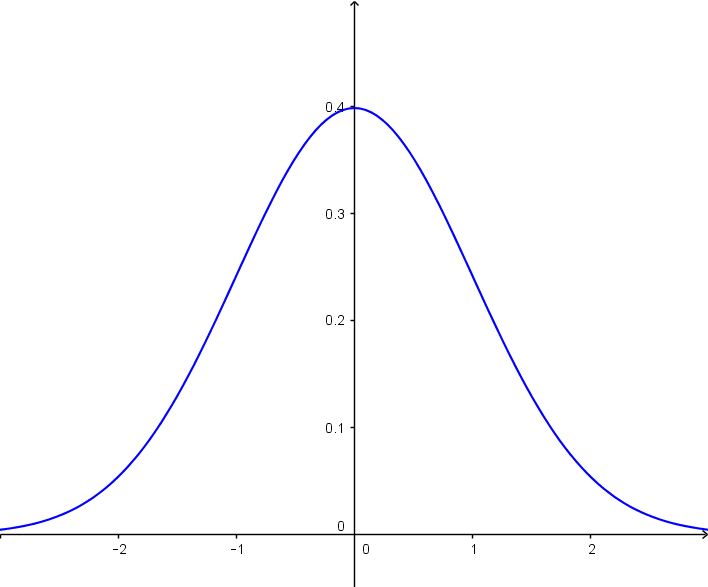
\includegraphics[width=0.8\textwidth]{img/gauss}
    \caption{Gaussian Function plot with $\mu = 1$ and $\sigma = 1$}
    \label{fig-gauss}
\end{figure}

This particular function is advantageous to averaging out colour values across a surface, since it tends towards zero the farther away we get from our central point, and it does so on a smooth curve. An alternative method in which we took the naïve average over a radius would create blocky artefacts, since values at the edge would count the same as values closer to our central point.

\subsubsection{Image Filter}
We wish to fit the Gaussian Function to filter our radiosity and AO outputs, and a simple way to do so is to loop over all neighbouring pixels within radius $R$, and weigh their sampled values by the Gaussian of their distance to $P_c$. If we consider $B\prime(P_c)$ the filtered radiosity output for our point $P_c$, then we would find that value like so:

$$B\prime(P_c) = \frac{1}{W} \sum_{i = -R}^{R} \sum_{j = -R}^{R} G(|(i,j)|) \cdot B(P(i,j))$$
$$W = \sum_{i = -R}^{R} \sum_{j = -R}^{R} G(|(i,j)|)$$

We divide by the sum of all Gaussian weight values, since we're essentially doing a weighted average with the Gaussian Function as our weight.

Finally, we need to pick out the proper values of $\mu$ and $\sigma$. If we consider the distance from our central point to as the argument to $G(x)$, then we set $\mu = 0$. This means that our central point, $x = 0$, will have the highest weight. The standard deviation $\sigma$ will have to be picked such that our farthest point, $R$ is very close to zero. It is typical to say that this happens after three standard deviations, and as such we get $\sigma = \frac{R}{3}$. Figure \ref{fig-gauss-applied} demonstrates the application of this algorithm to a 11x11 image with a single white pixel in the center. The color of the center pixel has been spread across the other pixels according to a Gaussian distribution.

\begin{figure}[!ht]
  \centering
    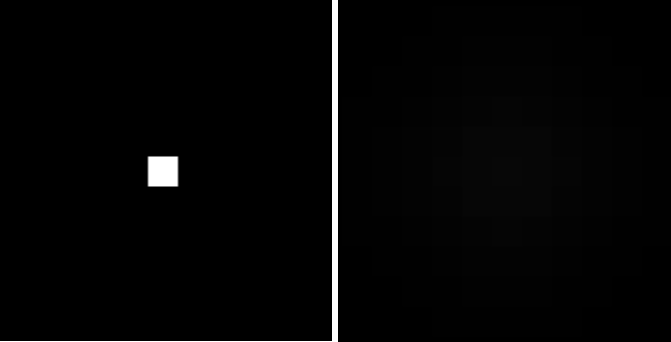
\includegraphics[width=0.8\textwidth]{img/gauss-pixel}
    \caption{The Gaussian filter applied to an 11x11 black square with a single white pixel. Right hand side is after the 									filter has been applied}
    \label{fig-gauss-applied}
\end{figure}

One quick performance improvement is to remove the factor $\frac{1}{\sigma \sqrt{2\pi}}$ from the Gaussian function since it is eliminated from the equation when we divide by $W$. As such we are left with the following function to replace $G(x)$

$$\gamma(x) = e ^ {-\frac{(x - \mu)^2}{2\sigma^2}}$$

\subsubsection{Modifications}
Running a filter over a full rectangle for every pixel would have a complexity of $O(n^2)$, where $n=2R + 1$. This is infeasible for large radii. Additionally, we want to employ some method of avoiding surfaces "bleeding" into each other. One way to achieve the latter to employ a bilateral filter\cite{bilat}, in which some function value of difference in intensity between two pixels is added as a factor to the weight of a pixel. One problem with this approach, however, is that it our final radiosity and AO results both have big differences between pixels on the same surface. As such, we will in stead employ a function of the depth difference between the two. We would like to also use the normal in some capacity, to accommodate adjacent but differently facing surfaces, but the results don't seem to be worth the extra loss in performance. In other words we add the term $Z_{factor}(x,y) = (1 - ||Z_{xy} - Z_{P_c}||)$ to the weight of a given sample point.

In terms of performance, we will turn the filter into a 2-pass one in stead of the original 1-pass. That is to say, in stead of polynomial complexity, we wish to make it linear. Essentially we wish to swap the original equation for our Gaussian weight with the following:

$$B\prime_{1st}(P_{c}) = \frac{1}{W} \sum_{i = -R}^{R} \gamma(i) Z_{factor} B(P(i,0))$$
$$B\prime(P_{c}) = \frac{1}{W} \sum_{i = -R}^{R} \gamma(i) Z_{factor} (x,y) B\prime_{1st}(P(0,i))$$
$$W = \sum_{i = -R}^{R} Z_{factor}(x,y) \gamma(i)$$

This filter runs in O(n) time and is thus much more suitable for averaging out large surfaces.  It also removes the use of length as an argument to the gaussian function, since we can now just use the value of $i$ as the argument.
\chapter{Implementation}
\section{Design Overview}
All code written for this project is part of an overall framework I wrote myself, which maintains everything that is not directly relevant to the project at hand. As such, I will not document the framework itself in-depth here. In general it manages camera movement based on input, timings, drawing and handling of debug console input etc. Most of this is handled through a rudimentary messaging system that manages data sent between different parts of the application..In this section I will start out by going through some general utility used broadly in the application, go through the central RenderEngine class, and finally explain, in broad strokes, how the different implemented filters function.

\section{General Utility}

\paragraph{The Full-Screen Quad (FSQuad}
Every time I apply an effect through deferred rendering I need to rasterise a full-screen quad. To ease this process, I have defined a static class in MyUtility.h that initialises a Vertex Array Object (VAO) for a full-screen quad, as well as its projection-view matrix. This allows me to just bind the VAO, and get the PV matrix without having to have local copies for applying every one of the filters. I am effectively trading performance for less code clutter with this, since accessing a static element in memory is generally slower than a class accessing a member.

The class is defined like so:
\begin{lstlisting}[caption={MyUtility.h},language=c++]
class FSQuad {
public:
    static void setupQuad();
    static GLuint getVAO();
    static const glm::mat4& getPV();
    static GLuint getNoIndices();
private:
    static glm::mat4 PV;
    static GLuint VAO;
    static GLuint noIndices;
};
\end{lstlisting}

And VAO and PV are initialised like so:
\begin{lstlisting}[caption={MyUtility.cpp},language=c++]
void FSQuad::setupQuad(){


	std::vector<Vertex> vertices = {Vertex(glm::vec3(-0.5f,-0.5f,0),glm::vec3(0,0,-1),glm::vec2(0,0)),
									Vertex(glm::vec3(-0.5f,0.5f,0),glm::vec3(0,0,-1),glm::vec2(0,1)),
									Vertex(glm::vec3(0.5f,-0.5f,0),glm::vec3(0,0,-1),glm::vec2(1,0)),
									Vertex(glm::vec3(0.5f,0.5f,0),glm::vec3(0,0,-1),glm::vec2(1,1))
	};

	std::vector<GLuint> indices = {0,1,2,1,2,3};

	MeshObject quad = MeshObject(vertices,indices);

	VAO = quad.getVAO();

	PV = glm::ortho( -0.5f,0.5f,-0.5f,0.5f,-1.0f,1.0f)*
		 glm::lookAt(glm::fvec3(0,0,0),glm::fvec3(0,0,-1),glm::fvec3(0,1,0));

	noIndices = quad.getNoIndices();
}
\end{lstlisting}
It is important that \verb=FSQuad::setupQuad()= is run somewhere in the program \emph{before} it is used.

\paragraph{Mesh Object}
The Mesh Object class manages a single mesh. Its constructor takes either dynamic arrays of geometry data or AssImp data pointers to generate a VAO that holds information on vertex attribute locations. It also save the total number of indices in the element buffer. I interleave the geometric data because it's much more effective than uploading the data into separate arrays. Here's the VAO generation:

\begin{lstlisting}[caption={MeshObject.cpp},language=c++]
void MeshObject::setupVAO(std::vector<Vertex> const &vertices, std::vector<GLuint> const &indices) {
    glGenVertexArrays(1, &vao);
    glBindVertexArray(vao);

    GLuint vbuffer;
    glGenBuffers(1, &vbuffer);
    glBindBuffer(GL_ARRAY_BUFFER, vbuffer);

    glBufferData(GL_ARRAY_BUFFER, vertices.size() * sizeof(Vertex), &(vertices[0]), GL_STATIC_DRAW);

    glEnableVertexAttribArray(0);
    glVertexAttribPointer(0, 3, GL_FLOAT, GL_FALSE, sizeof(Vertex), (void*)offsetof(Vertex, position));
    glEnableVertexAttribArray(1);
    glVertexAttribPointer(1, 3, GL_FLOAT, GL_FALSE, sizeof(Vertex), (void*)offsetof(Vertex, normal));
    glEnableVertexAttribArray(2);
    glVertexAttribPointer(2, 2, GL_FLOAT, GL_FALSE, sizeof(Vertex), (void*)offsetof(Vertex, UV));

    GLuint ibuffer;
    glGenBuffers(1, &ibuffer);
    glBindBuffer(GL_ELEMENT_ARRAY_BUFFER, ibuffer);

    glBufferData(GL_ELEMENT_ARRAY_BUFFER, indices.size() * sizeof(GLuint), &(indices[0]), GL_STATIC_DRAW);

    glBindVertexArray(0);

    noIndices = indices.size();

    std::cout << "A new mesh was added with " << noIndices << " indices" << std::endl;
}
\end{lstlisting}

I use a standardised vertex format in which vertex positions are at location 0, normals at location 1 and UVs (when relevant) are at location 2.

\paragraph{Universal Shaders}
I have a number of universal vertex and geometry shaders that are used to rasterise the full-screen quad for deferred rendering. Which I use for a certain purpose depends primarily on whether or not the render target or source texture are layered. The following vertex shader is used to rasterize a quad when the render-target is single-layered:
\begin{lstlisting}[caption={unlayered\_texture.vert},language=GLSL]
#version 330

layout(location=0)in vec3 position;
layout(location=2)in vec2 UVIn;

uniform mat4 pvm;

out vec2 UV;
out vec4 pos;

void main() {
    pos = pvm * vec4(position,1);
    gl_Position = pos;
    UV = UVIn;
}
\end{lstlisting}

The only difference between this and the one intended for 2-layered render targets, is that the latter does not set \verb=gl_Position=, since that is done in the geometry shader:

\begin{lstlisting}[caption={layered\_quad.geom},language=GLSL]
#version 330

layout(triangles) in;
layout(triangle_strip, max_vertices=6) out;

in vec2 UV[];
in vec4 pos[];

out vec2 fragUV;
out vec2 windowSpace;
flat out int layer;

void main() {
    gl_Layer = 0;
    layer = 0;
    for(int i = 0; i < 3; i++) {
        gl_Position = pos[i];
        fragUV = UV[i];
        EmitVertex();
    }
    EndPrimitive();

    gl_Layer = 1;
    layer = 1;
    for(int i = 0; i < 3; i++) {
        gl_Position = pos[i];
        fragUV = UV[i];
        EmitVertex();
    }
    EndPrimitive();
}
\end{lstlisting}

I draw to the backbuffer with one of two fragment shaders based on whether or not the texture being drawn is layered. For layered textures it is possible to change layer with the command \verb=drawlayer X=, where \verb=X= is either 0 or 1.

\begin{lstlisting}[caption={layered\_texture.frag},language=GLSL]
#version 330

in vec2 UV;

uniform sampler2DArray texture_uniform;
uniform int layer;

out vec4 fragColor;

void main() {
    fragColor = texture(texture_uniform, vec3(UV,layer)).rgba;
}
\end{lstlisting}

The only difference for non-layered textures is that the \verb=sampler2DArray= is a \verb=sampler2D=, and I index into it with just the UVs.

\section{The RenderEngine Class}
\verb=RenderEngine.h= and \verb=RenderEngine.cpp=

The RenderEngine class is the central piece in the rendering loop. That is to say its main purpose is to be a collector of all scene information, the g-buffer and filters. It also ensures that all relevant elements have been initialised and updates the backbuffer every frame and ensures that all relevant filters have been run.

This is the RenderEngine initialisation function:
\begin{lstlisting}[caption={RenderEngine.cpp},language=c++]
bool RenderEngine::initEngine(int width, int height) {

	this->width = width;
	this->height = height;

	glfwSetInputMode(context,GLFW_CURSOR,GLFW_CURSOR_DISABLED);

	glViewport(0,0,width,height);
	glClearColor(0,0,0,1);

	updateBuffers(context,width,height);

	parseImportFile("res/models/cornell-box/CornellBox-Original.obj");

	lights.push_back(Light(glm::vec3(0.0f,1.8f,0.0f),glm::vec3(4.0f,4.0f,4.0f)));

	dbg.addTimer(time.getName(),time.getAvgTimePtr());
	time.activate();

	initTextures(width,height);

	FSQuad::setupQuad();

	check_gl_error();
}
\end{lstlisting}
It sets the viewport, ensures that all buffers have the right dimensions, imports geometry from a file, adds a light and sets up a timer. While FSQuad is a static class and not a member of RenderEngine, I consider it under its responsibilities to initialise it. It also initialises all the textures containing the final results produced by the filters:

\begin{lstlisting}[caption={RenderEngine.cpp},language=c++]
glBindTexture(GL_TEXTURE_2D_ARRAY,radTot);

glTexParameteri(GL_TEXTURE_2D_ARRAY,GL_TEXTURE_MIN_FILTER,GL_LINEAR);
glTexParameteri(GL_TEXTURE_2D_ARRAY,GL_TEXTURE_MAG_FILTER,GL_LINEAR);
glTexParameteri(GL_TEXTURE_2D_ARRAY,GL_TEXTURE_WRAP_S,GL_CLAMP_TO_EDGE);
glTexParameteri(GL_TEXTURE_2D_ARRAY,GL_TEXTURE_WRAP_T,GL_CLAMP_TO_EDGE);

glTexImage3D(GL_TEXTURE_2D_ARRAY,0,GL_R11F_G11F_B10F,width,height,2,0,GL_RGB,GL_FLOAT,0);

glGenTextures(1, &radPrev);
glBindTexture(GL_TEXTURE_2D_ARRAY,radPrev);

glTexParameteri(GL_TEXTURE_2D_ARRAY,GL_TEXTURE_MIN_FILTER,GL_LINEAR);
glTexParameteri(GL_TEXTURE_2D_ARRAY,GL_TEXTURE_MAG_FILTER,GL_LINEAR);
glTexParameteri(GL_TEXTURE_2D_ARRAY,GL_TEXTURE_WRAP_S,GL_CLAMP_TO_EDGE);
glTexParameteri(GL_TEXTURE_2D_ARRAY,GL_TEXTURE_WRAP_T,GL_CLAMP_TO_EDGE);

glTexImage3D(GL_TEXTURE_2D_ARRAY,0,GL_R11F_G11F_B10F,width,height,2,0,GL_RGB,GL_FLOAT,0);

glBindTexture(GL_TEXTURE_2D_ARRAY,0);

glGenTextures(1, &alchAO);
glBindTexture(GL_TEXTURE_2D,alchAO);

glTexParameteri(GL_TEXTURE_2D,GL_TEXTURE_MIN_FILTER,GL_LINEAR);
glTexParameteri(GL_TEXTURE_2D,GL_TEXTURE_MAG_FILTER,GL_LINEAR);
glTexParameteri(GL_TEXTURE_2D,GL_TEXTURE_WRAP_S,GL_CLAMP_TO_EDGE);
glTexParameteri(GL_TEXTURE_2D,GL_TEXTURE_WRAP_T,GL_CLAMP_TO_EDGE);

glTexImage2D(GL_TEXTURE_2D,0,GL_R32F,width,height,0,GL_RED,GL_FLOAT,0);

glBindTexture(GL_TEXTURE_2D,0);
\end{lstlisting}
I use \verb=11_11_10= textures for the radiosity targets, which are float textures with 11-bit precision for red and green channels and 10 bits of precision for the blue channel. They take up the same amount of memory as RGBA textures, but allow more precision. I have both a total and a previous bounce target for radiosity, since I need the previous bounce to calculate subsequent bounces of radiosity.

\begin{lstlisting}[caption={RenderEngine.cpp},language=c++]
void RenderEngine::draw() {

    dt = glfwGetTime() - prevTime;
    prevTime = glfwGetTime();

    static LambertianFilter lambert = LambertianFilter(width,height,radPrev,radTot);
    static RadiosityFilter radFilter = RadiosityFilter(width,height,radPrev,radTot);
	static AOFilter ssaoFilter = AOFilter(width,height,alchAO);	
	
    parseRenderMessages();

    cam.update();

    time.startTimer();

    buffer.generate(&meshes, &cam);

    for(int i = 0; i < lights.size(); i++) {
        lights[i].genShadowMap(&cam,&meshes);
    }

    glViewport(0,0,width,height);

    lambert.applyLambertian(&cam, &buffer, lights);
    for(int i = 0; i < bounces; i++) {
        radFilter.applyBounce(&cam,&buffer);
    }

    time.endTimer();

    glClearColor(0,1,0,1);

    glBindFramebuffer(GL_DRAW_FRAMEBUFFER,0);
    glClear(GL_DEPTH_BUFFER_BIT | GL_COLOR_BUFFER_BIT);

    //Render to backbuffer.

    //Render to backbuffer.
	if(backBufferTexture != -1)
		renderTextureLevel(backBufferTexture,backBufferLayer);
	else
		renderComposite();

    dbg.draw();

    glfwSwapBuffers(context);

    check_gl_error();
}
\end{lstlisting}
The most relevant part of the class is the \verb=draw()= function, which tells the light and G-buffer to generate their respective textures, such that they are ready to be used for the filters. It then runs all filters before drawing to the backbuffer. Whether to draw the final composited image or an off-screen buffer, and which buffer to draw, can be set with console commands. All filters are static members of the function, since there's no need for them outside of it. When they are constructed, they also receive any target or source texture they may need that are not part of the G-buffer or themselves exclusively. This is done to allow for the FBO to be set up once, without needing to swap around colour attachments.

If the user has asked for an off-screen buffer, the following function makes sure to draw it to the backbuffer:
\begin{lstlisting}[caption={RenderEngine.cpp},language=c++]
void RenderEngine::renderTextureLevel(GLuint texture, unsigned short int layer) {
	static Shader::ShaderProgram tex_shader = Shader::ShaderProgram("../shaders/texture_quad.vert","../shaders/layered_texture.frag");
	static Shader::ShaderProgram nolayers_tex_shader = Shader::ShaderProgram("../shaders/texture_quad.vert","../shaders/unlayered_texture.frag");

	glBindVertexArray(FSQuad::getVAO());

	glm::mat4 pvm = FSQuad::getPV();

	if(isLayered) {

		tex_shader.use();

		glUniformMatrix4fv(tex_shader.get_U_Location(Shader::U_M_PVM), 1, GL_FALSE, glm::value_ptr(pvm));

		glActiveTexture(GL_TEXTURE0);
		glBindTexture(GL_TEXTURE_2D_ARRAY, texture);
		glUniform1i(tex_shader.get_U_Location(Shader::U_I_TEXTURE), 0);

		glUniform1i(tex_shader.get_U_Location(Shader::U_I_LAYER), layer);

		glDrawElements(GL_TRIANGLES, FSQuad::getNoIndices(), GL_UNSIGNED_INT, (void *) 0);
	} else {

		nolayers_tex_shader.use();

		glUniformMatrix4fv(nolayers_tex_shader.get_U_Location(Shader::U_M_PVM), 1, GL_FALSE, glm::value_ptr(pvm));

		glActiveTexture(GL_TEXTURE0);
		glBindTexture(GL_TEXTURE_2D, texture);
		glUniform1i(nolayers_tex_shader.get_U_Location(Shader::U_I_TEXTURE), 0);

		glDrawElements(GL_TRIANGLES, FSQuad::getNoIndices(), GL_UNSIGNED_INT, (void *) 0);
	}
}
\end{lstlisting}
There are two different cases depending on whether or not the off-screen buffer is layered or not.

\section{The GBuffer Class}

The Gbuffer class constructor ensures that everything needed to generate our G-buffer is generated and initialised. The shader is initialised in the initialiser list. I use a geometry shader to emit primitives to both layers of the buffers.

\begin{lstlisting}[caption={GBuffer.cpp},language=c++]
GBuffer::GBuffer(int width, int height) :
gen_shader("../shaders/gen_gbuffer.vert","../shaders/gen_gbuffer.frag","../shaders/gen_gbuffer.geom")
{
	this->width = width;
	this->height = height;

	check_gl_error();

	setupTextures();

	check_gl_error();
}
\end{lstlisting}

The \verb=setupTextures()= function generates and sets up the FBO and textures. The textures are not actually tied to their relevant attachment points on the FBO yet, since I actually need to switch the depth attachment around every frame.
All texture initialisation is a variation of the following (sometimes they have different internal formats based on the type of data they need to contain):

\begin{lstlisting}[caption={GBuffer.cpp},language=c++]
glGenTextures(1, &depths);
glBindTexture(GL_TEXTURE_2D_ARRAY,depths);

glTexParameteri(GL_TEXTURE_2D_ARRAY,GL_TEXTURE_MIN_FILTER,GL_NEAREST);
glTexParameteri(GL_TEXTURE_2D_ARRAY,GL_TEXTURE_MAG_FILTER,GL_NEAREST);
glTexParameteri(GL_TEXTURE_2D_ARRAY,GL_TEXTURE_WRAP_S,GL_CLAMP_TO_EDGE);
glTexParameteri(GL_TEXTURE_2D_ARRAY,GL_TEXTURE_WRAP_T,GL_CLAMP_TO_EDGE);

glTexImage3D(GL_TEXTURE_2D_ARRAY,0,GL_DEPTH_COMPONENT32F,width,height,2,0,GL_DEPTH_COMPONENT,GL_FLOAT,0);
\end{lstlisting}

All render target textures in the product are set with the filtering as \verb=GL_NEAREST=, since linear filtering can cause some weird results with deferred rendering targets. The G-buffer class has a total of five textures, normals, diffuse reflectance, specular reflectance and two depth buffers. I use 32-bit float depth components to get more precision when regenerating positions.

Once setup is done, the function \verb=generate()= takes a dynamic array of meshes and a camera to write the geometry data to its textures. First it sets up its render targets

\begin{lstlisting}[caption={GBuffer.cpp},language=c++]
glBindFramebuffer(GL_DRAW_FRAMEBUFFER, FBO);

currentState = !currentState;

GLuint activeDepth = currentState ? depths : depths2;
GLuint depthToPass = currentState ? depths2 : depths;

glFramebufferTexture(GL_DRAW_FRAMEBUFFER,GL_DEPTH_ATTACHMENT,activeDepth,0);
glFramebufferTexture(GL_DRAW_FRAMEBUFFER,GL_COLOR_ATTACHMENT0,normals,0);
glFramebufferTexture(GL_DRAW_FRAMEBUFFER,GL_COLOR_ATTACHMENT1,diffColors,0);
glFramebufferTexture(GL_DRAW_FRAMEBUFFER,GL_COLOR_ATTACHMENT2,specColors,0);

GLuint buffers[3] = {GL_COLOR_ATTACHMENT0,GL_COLOR_ATTACHMENT1,GL_COLOR_ATTACHMENT2};

glDrawBuffers(3,buffers);
\end{lstlisting}

I swap around the depth attachment each frame, so that I can use that of the previous frame to determine whether or not a fragment belongs in the second layer.

After this has been done, I bind the shader, clear the depth and colour buffers and upload the uniforms needed for the generation in general, and loop through the meshes to draw them one at a time. For each mesh I set its diffuse and specular reflectance as uniforms. All models used are defined in such a way that no model matrix is needed.

\begin{lstlisting}[caption={GBuffer.cpp},language=c++]
[...]clear buffers, set states as needed

gen_shader.use();

glActiveTexture(GL_TEXTURE0);
glBindTexture(GL_TEXTURE_2D_ARRAY, depthToPass);
glUniform1i(gen_shader.get_U_Location(Shader::U_I_DEPTH_TEX),0);

[...]//Get projection and view matrices from Camera.

glUniformMatrix4fv(gen_shader.get_U_Location(Shader::U_M_VM),1,GL_FALSE,glm::value_ptr(vm));

glUniformMatrix4fv(gen_shader.get_U_Location(Shader::U_M_PVM),1,GL_FALSE,glm::value_ptr(pvm));

glUniform1f(gen_shader.get_U_Location(Shader::U_F_FARPLANE),cam->farPlane);
glUniform1f(gen_shader.get_U_Location(Shader::U_F_NEARPLANE),cam->nearPlane);

for(std::vector<MeshObject>::iterator iter = meshes->begin(); iter != meshes->end();iter++) {
	glBindVertexArray(iter->getVAO());

	glUniform4fv(gen_shader.get_U_Location(Shader::U_V4_DIFF_COL),1,glm::value_ptr(iter->diffColor));
	glUniform4fv(gen_shader.get_U_Location(Shader::U_V4_SPEC_COL),1,glm::value_ptr(iter->specColor));
	glDrawElements(GL_TRIANGLES,iter->getNoIndices(),GL_UNSIGNED_INT,(void*) 0);
}
\end{lstlisting}

My Shader class buffers all uniform addresses for a shader in a map, which you access with an \verb=enum=, which is why the uniform uploads might look a little wonky. Once the scene has been drawn, the G-buffer textures are ready to be used. I use the following shaders for the pipeline. The vertex shader is fairly par for the course:

\begin{lstlisting}[caption={gen\_gbuffer.vert},language=GLSL]
#version 330

layout(location=0) in vec3 position;
layout(location=1) in vec3 normal;

uniform mat4 pvm;
uniform mat4 vm;

out vec3 outNormal;
out vec4 outPos;
out vec2 screenUV;
out vec4 screenPos;

void main() {
	outNormal = mat3(vm) * normal;
	outPos = pvm * vec4(position,1);
	screenPos = vm * vec4(position,1);
	screenUV = vec4((outPos/outPos.w + 1) / 2).xy;
}
\end{lstlisting}

The only slightly unusual thing here is that I use \verb=layout(location)= qualifiers for the vertex attributes. I do this because it allows me to have a standardised vertex format, whereby when I set up the attribute pointers for a VAO, I know that positions are in location 0, normals in position 1 and UVs (if it has any) are in position 2. This also allows me to not set vertex attribute pointers every time I draw the scene which leads to better performance and cleaner code. The geometry shader was posted (in large parts at least) in the theory section \ref{list-deepgeom}, this is how it looks specifically:

\begin{lstlisting}[caption={gen\_gbuffer.geom},language=GLSL]
out vec3 normalIn;
noperspective out vec2 screenUVFrag;
out vec3 screenPosFrag;
flat out int layer;

void main() {
	layer = 0;
	gl_Layer = 0;
	for(int i = 0; i < 3; i++) {
		normalIn = outNormal[i];
		screenUVFrag = screenUV[i];
		screenPosFrag = vec3(screenPos[i]);
		gl_Position = outPos[i];
		EmitVertex();
	}
	EndPrimitive();
	
	layer = 1;
	gl_Layer = 1;
	for(int i = 0; i < 3; i++) {
		normalIn = outNormal[i];
		screenUVFrag = screenUV[i];
		screenPosFrag = vec3(screenPos[i]);
		gl_Position = outPos[i];
		EmitVertex();
	}
	EndPrimitive();
}
\end{lstlisting}

All this does is relay the information calculated in the vertex shader to the fragment shader twice, once for each layer. I use the \verb=noperspective= interpolation qualifier on the screen UV coordinates, since they are linear in screen space. Finally, the fragment shader writes to the colour attachments. The fragment shader is fairly big, so I will not list it in its entirety here. The most important part of it is this:

\begin{lstlisting}[caption={gen\_gbuffer.frag},language=GLSL]
switch(layer) {
case 0:
	normal = normalize(normalIn).xyz;
	diffColor = vec4(diff_color.xyz,1.0f);
	specColor = vec4(spec_color.xyz,spec_color.w/128.0f);
break;
case 1:

	if(linearDepth(gl_FragCoord.z) <= linearDepth(texture(depth_texture,vec3(screenUVFrag,0)).r) + 0.01f)
		discard;
	else {
		normal = normalize(normalIn).xyz;
		diffColor = vec4(diff_color.xyz,1.0f);
		specColor = vec4(spec_color.xyz,spec_color.w/128.0f);
	}
break;
}
\end{lstlisting}

What this means is that for fragments being written to layer 1 of our G-buffer, it writes the data as it would with a regular flat G-buffer. If it is being written to layer 2, however, it tests to see if it lies behind the minimal layer of separation ($0.01$ here) from the first layer of the comparison depth buffer, write the data, otherwise discard the fragment. I write the shininess of the material to the alpha channel of the specular colour divided by 128. Not having this in a separate texture with more precision means that there is only going to be 255 discretely different possible exponents. Since the shininess was never meant to give precise reflections (at least not in a rasteriser pipeline,) however, this imprecision is of minimal importance.

In order to gain access to the G-buffer textures, other classes can use the \verb=getBuffer()= function that takes an enum representing a buffer, and returns the pointer (\verb=GLuint=) to the texture.

\section{Direct Lighting and Shadowmap}

Shadow map generation is managed by the Light class in \verb=light.cpp=. They are generated by rasterising the geometry of the scene unto a cube-map in a single pass. In order to do so, I first need to set up the proper look-ats for every direction of the cube map, which is done like this:
\begin{lstlisting}[caption={light.cpp},language=c++]
glm::mat4 projection = glm::perspective(glm::pi<float>()/2.0f,1.0f,cam->nearPlane,cam->farPlane);

glm::mat4 pvms[6] = {projection * glm::lookAt(position,position + glm::vec3(1.0f,0.0f,0.0f),glm::vec3(0.0f,-1.0f,0.0f)),
           projection * glm::lookAt(position,position + glm::vec3(-1.0f,0.0f,0.0f),glm::vec3(0.0f,-1.0f,0.0f)),
           projection * glm::lookAt(position,position + glm::vec3(0.0f,1.0f,0.0f),glm::vec3(0.0f,0.0f,1.0f)),
           projection * glm::lookAt(position,position + glm::vec3(0.0f,-1.0f,0.0f),glm::vec3(0.0f,0.0f,-1.0f)),
           projection * glm::lookAt(position,position + glm::vec3(0.0f,0.0f,1.0f),glm::vec3(0.0f,-1.0f,0.0f)),
           projection * glm::lookAt(position,position + glm::vec3(0.0f,0.0f,-1.0f),glm::vec3(0.0f,-1.0f,0.0f))
};

glm::mat4 vms[6] = {glm::lookAt(position,position + glm::vec3(1.0f,0.0f,0.0f),glm::vec3(0.0f,-1.0f,0.0f)),
          glm::lookAt(position,position + glm::vec3(-1.0f,0.0f,0.0f),glm::vec3(0.0f,-1.0f,0.0f)),
          glm::lookAt(position,position + glm::vec3(0.0f,1.0f,0.0f),glm::vec3(0.0f,0.0f,1.0f)),
          glm::lookAt(position,position + glm::vec3(0.0f,-1.0f,0.0f),glm::vec3(0.0f,0.0f,-1.0f)),
          glm::lookAt(position,position + glm::vec3(0.0f,0.0f,1.0f),glm::vec3(0.0f,-1.0f,0.0f)),
          glm::lookAt(position,position + glm::vec3(0.0f,0.0f,-1.0f),glm::vec3(0.0f,-1.0f,0.0f))
};

glUniformMatrix4fv(program.get_U_Location(Shader::U_M_PVM),6,GL_FALSE,glm::value_ptr(pvms[0]));

glUniformMatrix4fv(program.get_U_Location(Shader::U_M_VM),6,GL_FALSE,glm::value_ptr(vms[0]));
\end{lstlisting}
I generate view-matrices on top of projection-view matrices, since I need the view-matrix to determine the length of the position vector. The indices of the matrices were found in accordance with the OpenGL cubemap specification.

When the projection-view matrices have been generated I loop through all geometry passed to the function and draw them to the cube map.
\begin{lstlisting}[caption={light.cpp},language=c++]
glUniform1f(program.get_U_Location(Shader::U_F_FARPLANE),cam->farPlane);

for(std::vector<MeshObject>::iterator iter = meshes->begin(); iter != meshes->end();iter++) {
  glBindVertexArray(iter->getVAO());

  glDrawElements(GL_TRIANGLES,iter->getNoIndices(),GL_UNSIGNED_INT,(void*) 0);
}
\end{lstlisting}

In order to do the generation in a single step, I need a geometry shader that simply loops through primitives six times, to relay the geometry to the fragment shader for all six layers of the cube map:
\begin{lstlisting}[caption={shadow\_gen.geom},language=GLSL]
#version 330

layout(triangles) in;
layout(triangle_strip, max_vertices=18) out;

in vec4 outPos[];

uniform mat4 pvm[6];
uniform mat4 vm[6];

out vec3 fragPos;

void main() {
	for(int i = 0; i < 6; i++) {
		gl_Layer = i;
		for(int j = 0; j < 3; j++) {
			fragPos = (vm[i] * outPos[j]).xyz;

			gl_Position = pvm[i] * outPos[j];
			EmitVertex();
		}
		EndPrimitive();
	}
}
\end{lstlisting}

Finally I write the length of the interpolated verex position divided by the far plane to the fragment. I divide by the far plane, since depth component values run between 0 and 1.
\begin{lstlisting}[caption={shadow\_gen.frag},language=GLSL]
#version 330

in vec3 fragPos;

uniform float far_plane;

void main() {
	gl_FragDepth = length(fragPos)/far_plane;
}
\end{lstlisting}

Once I have the shadow map, I can run the Lambertian shader. In order to reconstruct the position and find the world-space coordinates needed to determine occlusion, I need to upload the inverse projection matrix as well as the inverse view-matrix:
\begin{lstlisting}[caption={Filters.cpp},language=c++]
glm::mat4 invProjection = glm::inverse(cam->getProjection());

glUniformMatrix4fv(program.get_U_Location(Shader::U_M_VUNPROJECT),1,GL_FALSE,glm::value_ptr(invProjection));

glUniformMatrix4fv(program.get_U_Location(Shader::U_M_UNVIEW),1,GL_FALSE,glm::value_ptr(glm::inverse(cam->getLookAt())));
\end{lstlisting}

I then loop through all light sources with additive blending enabled, to get both direct illumination as well as the value I will use to determine the first radiosity bounce. This is possible because I're using deferred rendering.
\begin{lstlisting}[caption={Filters.cpp},language=c++]
for(int i = 0; i < lights.size(); i++) {
  glm::vec3 lightPos = lights[i].getPosition();
  glm::vec3 lightIntensity = lights[i].getIntensity();

  glUniform3fv(program.get_U_Location(Shader::U_V3_LIGHTPOS), 1, glm::value_ptr(lightPos));

  glUniform3fv(program.get_U_Location(Shader::U_V3_LIGHT_INTENSITY), 1, glm::value_ptr(lightIntensity));

  glActiveTexture(GL_TEXTURE3);
  glBindTexture(GL_TEXTURE_CUBE_MAP,lights[i].getShadowMap());
  glUniform1i(program.get_U_Location(Shader::U_I_SHADOWMAP),3);

  check_gl_error();

  glDrawElements(GL_TRIANGLES, FSQuad::getNoIndices(), GL_UNSIGNED_INT, (void *) 0);
}
\end{lstlisting}

The fragment shader used to determine the Lambertian term is \verb=lambert.frag=. In order to determine the position, I need to reconstruct it from the depth. For this I use the following function, which is a direct implementation of the function described under Theory.
\begin{lstlisting}[language=GLSL]
vec3 regenPos(float tex_depth, vec2 winSpace) {
	vec4 v_screen = vec4(winSpace.xy,tex_depth,1.0);
	vec4 v_homo = viewUnproject * (2.0 * (v_screen - vec4(0.5)));

	return v_homo.xyz/v_homo.w;
}
\end{lstlisting}

I determine the world-space position by first reconstructing it from the depth buffer, and then multiplying it by the inverse view matrix. The normal is read directly and then multiplied by a \verb=mat3=-casted inverse view matrix (since it's a direction.)
\begin{lstlisting}[caption={lambert.frag},language=GLSL]
float Z_value = texture(depth_texture,vec3(fragUV.xy,float(layer))).r;

if(Z_value == 1.0f) {
  nextBounce = vec3(0.0f);
  total = vec3(0.0f);
  discard;
}

vec3 viewPos = regenPos(Z_value,fragUV.xy);
vec4 diff_color = texture(diff_texture,vec3(fragUV.xy,float(layer)));
vec3 viewNormal = texture(norm_texture,vec3(fragUV.xy,float(layer))).xyz;

vec3 worldPos = vec4(invView * vec4(viewPos,1.0f)).xyz;
vec3 worldNorm = mat3(invView) * viewNormal;
\end{lstlisting}

I now have all the values needed to do our lambertian shading. I multiply the lambertian by an attenuation value which varies depending on the scene and the visibility factor. I find the visibility factor by looking up in the shadow map in the direction of the negative \verb=lVector= and comparing that value to the length of the vector from the position to the light divided by the far plane. I subtract a bias to avoid shadow acne. If the depth is closer to or equal length from the light source as the depth value written to the shadow map, the point is not occluded.
\begin{lstlisting}[caption={lambert.frag},language=GLSL]
vec3 plVector = light_pos - worldPos;
vec3 lVector = normalize(plVector);
float atten = length(plVector);

float shadowDepth = texture(shadowMap,-lVector).r;

float depthToCompare = length(plVector)/far_plane;

float V = 0.0f;

if(depthToCompare - BIAS <= shadowDepth)
  V = 1.0f;

vec3 radValue = dot(lVector,worldNorm)*(vec3(diff_color)/M_PI)*light_intensity;

nextBounce = (1.0f/(0.5 + 0.7f * atten*atten)) * radValue * V;
total = (1.0f/(0.5 + 0.7f * atten*atten)) * radValue * V;
\end{lstlisting}

\section{Filters}
\subsection{Radiosity}
The C++ side of the radiosity filter is fairly straight-forward. It sets up the full-screen quad, and uploads the five different textures needed to calculate the next bounce of radiosity. \verb=randTex= is an \verb=R32F= texture containing random values between 0 and $2\pi$ to determine what value to rotate the spiral by when I sample, that is to say $\phi$. The values are unique for each fragment.
\begin{lstlisting}[caption={Filters.cpp},language=c++]
void RadiosityFilter::applyBounce(Camera *cam, GBuffer *buffer) {
	glBindFramebuffer(GL_DRAW_FRAMEBUFFER, FBO);

	glDisable(GL_DEPTH_TEST);

	program.use();

	glBindVertexArray(FSQuad::getVAO());

	glm::mat4 pvm = FSQuad::getPV();

	glm::mat4 invProjection = glm::inverse(cam->getProjection());

	glUniformMatrix4fv(program.get_U_Location(Shader::U_M_PVM),1,GL_FALSE,glm::value_ptr(pvm));

	glUniformMatrix4fv(program.get_U_Location(Shader::U_M_VUNPROJECT),1,GL_FALSE,
					   glm::value_ptr(invProjection));

	glActiveTexture(GL_TEXTURE0);
	glBindTexture(GL_TEXTURE_2D_ARRAY, buffer->getBuffer(e_depths));
	glUniform1i(program.get_U_Location(Shader::U_I_DEPTH_TEX),0);

	glActiveTexture(GL_TEXTURE1);
	glBindTexture(GL_TEXTURE_2D_ARRAY,buffer->getBuffer(e_normals));
	glUniform1i(program.get_U_Location(Shader::U_I_NORM_TEX),1);

	glActiveTexture(GL_TEXTURE2);
	glBindTexture(GL_TEXTURE_2D_ARRAY,buffer->getBuffer(e_diffColors));
	glUniform1i(program.get_U_Location(Shader::U_I_DIFF_TEX),2);

	glActiveTexture(GL_TEXTURE3);
	glBindTexture(GL_TEXTURE_2D_ARRAY,prevBounce);
	glUniform1i(program.get_U_Location(Shader::U_I_PREVRAD),3);

	glActiveTexture(GL_TEXTURE4);
	glBindTexture(GL_TEXTURE_2D,randTex);
	glUniform1i(program.get_U_Location(Shader::U_I_NOISE_TEX),4);

	glDrawElements(GL_TRIANGLES,FSQuad::getNoIndices(),GL_UNSIGNED_INT,(void*) 0);

	glBindFramebuffer(GL_DRAW_FRAMEBUFFER,0);

	glEnable(GL_DEPTH_TEST);

	gauss.applyGauss(buffer, tempRadTex);
}
\end{lstlisting}

This is how I find the values for the random texture:
\begin{lstlisting}[caption={Filters.cpp},language=c++]
for(unsigned long int i = 0; i < width*height; i++) {

	float angle = glm::linearRand<float>(0.0f, 2.0f * glm::pi<float>());
	randNoise[i] = angle;
}
\end{lstlisting}

The shader contains the array that determines how many spiral turns to do for a given number of samples from \cite{deep-g-buffer}. In order to determine the number of spiral turns to do I simply index into it by the number of samples - 1 (due to 0-indexing.)
\begin{lstlisting}[caption={apply\_rad\_bounce.frag},language=GLSL]
const int tau_array[ ] = {1, 1, 2, 3, 2, 5, 2, 3, 2, 3, 3, 5, 5,
3, 4, 7, 5, 5, 7, 9, 8, 5, 5, 7, 7, 7, 8, 5, 8, 11, 12, 7,
10, 13, 8, 11, 8, 7, 14, 11, 11, 13, 12, 13, 19, 17, 13,
11, 18, 19, 11, 11, 14, 17, 21, 15, 16, 17, 18, 13, 17,
11, 17, 19, 18, 25, 18, 19, 19, 29, 21, 19, 27, 31, 29, 21,
18, 17, 29, 31, 31, 23, 18, 25, 26, 25, 23, 19, 34, 19, 27,
21, 25, 39, 29, 17, 21, 27};

[...]

float tau = float(tau_array[SAMPLES - 1]);
\end{lstlisting}

First,I reconstruct the scene and initialise all values. Unlike the lambertian shader, positions and normals are reconstructed to view-space, since that is all I need. Unapplying the view-matrix would be an unnecessary cost. If no data has been written to the G-buffer textures the depth-buffer will be at its clear value (1.0,) and I do nothing for the fragment.
\begin{lstlisting}[caption={apply\_rad\_bounce.frag},language=GLSL]
float mainZ = texture(depth_texture,vec3(fragUV.xy,float(layer))).r;

if(mainZ == 1.0f) {
  nextBounce = vec3(0.0f);
  return;
}

vec3 mainPos = regenPos(mainZ,fragUV.xy);
vec4 mainColor = texture(diff_texture,vec3(fragUV.xy,float(layer)));
vec3 mainNormal = texture(norm_texture,vec3(fragUV.xy,float(layer))).xyz;


vec3 totalIrradiance = vec3(0);
float M = 0.0f;

float phi = texture(noise_tex,fragUV).r;
\end{lstlisting}

Once initialisation is done, I loop through the number of samples I want, in accordance with the spiral curve and radiosity equation explained in Theory. I only accept samples if they're on the hemisphere of the current fragment, are within screen-space and have had something written to them by the G-buffer.
\begin{lstlisting}[caption={apply\_rad\_bounce.frag},language=GLSL]
for(int i = 0; i < SAMPLES; i++) {

  float sigma_i = (i + 0.5f/tau)/float(SAMPLES);
  float theta_i = 2*M_PI*sigma_i*tau + phi;
  vec2 u_i = vec2(cos(theta_i),sin(theta_i));
  float h_i = RADIUS * sigma_i;

  vec2 offSet = vec2(h_i*u_i);

  vec2 offSetUV = fragUV.xy + vec2(offSet.x/WIN_WIDTH,offSet.y/WIN_HEIGHT);
  
  vec3 rad_1 = texture(prev_bounce,vec3(offSetUV,0.0)).rgb;
  float z_1 = texture(depth_texture,vec3(offSetUV,0.0)).r;
  vec3 pos_1 = regenPos(z_1,offSetUV);

  vec3 omega1 = pos_1 - mainPos;
  float geom1 = max(0,dot(normalize(omega1),mainNormal));

  vec3 rad_2 =  texture(prev_bounce,vec3(offSetUV,1.0)).rgb;
  float z_2 = texture(depth_texture,vec3(offSetUV,1.0)).r;
  vec3 pos_2 = regenPos(z_2,offSetUV);

  vec3 omega2 = pos_2 - mainPos;
  float geom2 = max(0,dot(normalize(omega2),mainNormal));
  
  if(geom1 > 0 &&
   abs(offSetUV.x - 0.5) <= 0.5 && abs(offSetUV.y - 0.5) <= 0.5 &&
   z_1 != 1.0f &&
   length(omega1) < 500.0) {
    M += 1.0f;
    totalIrradiance += rad_1.rgb * geom1;
  }

  if(geom2 > 0 &&
  abs(offSetUV.x - 0.5) <= 0.5 && abs(offSetUV.y - 0.5) <= 0.5 &&
  z_2 != 1.0f &&
  length(omega2) < 500.0) {
    M += 1.0f;
    totalIrradiance += rad_2.rgb * geom2;
  }

}

if(M > 0.1f)
  totalIrradiance = ((2.0f*M_PI)/M) * totalIrradiance;

vec3 radiosity = totalIrradiance * (mainColor.rgb/M_PI);

nextBounce = radiosity.rgb;
\end{lstlisting}

\subsection{SSAO}
The SSAO implementation is very similar to the radiosity one. The only difference is that the per-sample and total calculations have been replaced with the Alchemy AO algorithm\cite{VV11AlchemyAO}. The parameters of the equation change depending on the scene.
\begin{lstlisting}[caption={apply\_ssao.frag},language=GLSL]
if(geom1 > 0.0f &&
 abs(offSetUV.x - 0.5) <= 0.5 && abs(offSetUV.y - 0.5) <= 0.5 &&
 z_1 != 1.0f &&
 length(omega1) < OBSCURANCE_RADIUS) {
    totalAO += max(0,geom1 + mainPos.z * BETA)/(dot(omega1,omega1) + EPSILON);
    AO_samples += 1.0f;
}

if(geom2 > 0.0f &&
abs(offSetUV.x - 0.5) <= 0.5 && abs(offSetUV.y - 0.5) <= 0.5 &&
z_2 != 1.0f &&
length(omega2) < OBSCURANCE_RADIUS) {
    totalAO += max(0,geom2 + mainPos.z * BETA)/(dot(omega2,omega2) + EPSILON);
    AO_samples += 1.0f;
}
\end{lstlisting}

\verb=AO= is the fragment output value.
\begin{lstlisting}[caption={apply\_ssao.frag},language=GLSL]
if(AO_samples > 0.1f) {
    AO = pow(max(0,
                  1 - (((2*SIGMA)/AO_samples) * totalAO)),K);
} else
    AO = 1.0f;
\end{lstlisting}

I found the following parameters for the Cornell Box and the dragon to give the best results:
\begin{lstlisting}[language=c++]
#define EPSILON 1.0f
#define BETA 10e-4f
#define K 1.0f
#define SIGMA 2.0f
#define OBSCURANCE_RADIUS 0.1f
\end{lstlisting}
While the conference room scene has the following parameters:
\begin{lstlisting}[language=c++]
#define EPSILON 75.0f
#define BETA 10e-5f
#define K 2.0f
#define SIGMA 250.0f
#define OBSCURANCE_RADIUS 100.0f
\end{lstlisting}
These vary a lot compared to the parameters you usally see for the Alchemy SSAO, since the vertices defined in the OBJ-file have rather large values.

\subsection{Gaussian Filter}
\verb=filters.cpp=, \verb=bilat_hor.frag= and \verb=bilat_vert.frag=. The version for SSAO has a \verb=1ch= in its name to imply one channel input/output.

I apply the gaussian filter in a two-pass format. Due to this, I actually use two temporary textures to hold the intermediary results; one for the raw radiosity output, one for the result of the horizontal filter. The C++ code is very similar to the other deferred rendering filters. I set up the full-screen quad and upload the relevant buffer textures.
\begin{lstlisting}[caption={Filters.cpp},language=c++]
void GaussFilterWBlend::applyGauss(GBuffer *buffer, GLuint srcTex) {
	glDisable(GL_DEPTH_TEST);

	//Horizontal pass

	glBindFramebuffer(GL_DRAW_FRAMEBUFFER, FBO);

	program.use();
	glBindVertexArray(FSQuad::getVAO());

	glm::mat4 pvm = FSQuad::getPV();

	glUniformMatrix4fv(program.get_U_Location(Shader::U_M_PVM),1,GL_FALSE,glm::value_ptr(pvm));

	glActiveTexture(GL_TEXTURE0);
	glBindTexture(GL_TEXTURE_2D_ARRAY,srcTex);
	glUniform1i(program.get_U_Location(Shader::U_I_PREVRAD),0);

	glActiveTexture(GL_TEXTURE1);
	glBindTexture(GL_TEXTURE_2D_ARRAY,buffer->getBuffer(e_depths));
	glUniform1i(program.get_U_Location(Shader::U_I_DEPTH_TEX),1);

	glDrawElements(GL_TRIANGLES,FSQuad::getNoIndices(),GL_UNSIGNED_INT,(void*) 0);

	//Vertical pass

	glBindFramebuffer(GL_DRAW_FRAMEBUFFER,secondPassFBO);

	glEnablei(GL_BLEND,1);
	glBlendFunc(GL_ONE,GL_ONE);
	glBlendEquation(GL_FUNC_ADD);

	vert_shader.use();
	glBindVertexArray(FSQuad::getVAO());

	glUniformMatrix4fv(vert_shader.get_U_Location(Shader::U_M_PVM),1,GL_FALSE,glm::value_ptr(pvm));

	glActiveTexture(GL_TEXTURE0);
	glBindTexture(GL_TEXTURE_2D_ARRAY,tempTex);
	glUniform1i(vert_shader.get_U_Location(Shader::U_I_PREVRAD),0);

	glUniform1i(vert_shader.get_U_Location(Shader::U_I_DEPTH_TEX),1);

	glDrawElements(GL_TRIANGLES,FSQuad::getNoIndices(),GL_UNSIGNED_INT,(void*) 0);

	glDisablei(GL_BLEND,1);
	glDisable(GL_BLEND);

	glBindFramebuffer(GL_DRAW_FRAMEBUFFER,0);

	glEnable(GL_DEPTH_TEST);
}
\end{lstlisting}
You could argue that using two intermediary textures is superfluous and uses more VRAM than necessary. While this is true, I have decided to do it this way to make the code cleaner, easier to read and less interconnected. There're a couple of ways to get around this. One would be to have a single class manage all off-screen render targets, such that there is one or two in abundance. Another would be to swap around textures in the function itself such that the next bounce render target would change places every frame with the intermediary texture.

To apply the gaussian filter we use the Gaussian function defined in the Theory section.
\begin{lstlisting}[language=GLSL]
float gaussian(float x, float sigma) {
  return exp(-(x*x)/
        (2 * sigma * sigma));
}
\end{lstlisting}

I start by initialising values and ensuring that there is something written to the off-screen buffer at the current fragment position.
\begin{lstlisting}[caption={bilat\_hor.frag},language=GLSL]
vec3 total_contr = vec3(0);
float totalWeight = 0.0f;

float mainZ = texture(depth_texture,vec3(fragUV,float(layer))).r;

if(mainZ == 1.0f) {
  filtered = vec3(0,0,0);
  return;
}
\end{lstlisting}

Then, I loop through pixels horizontally, starting to the left of the current fragment. I sum up all contributions and their weights according to the gaussian function multiplied by an edge-correcting factor based on the depth. As the final step I make sure I'm not dividing by 0 and write the result to the fragment output.
\begin{lstlisting}[caption={bilat\_hor.frag},language=GLSL]
for(int i = -FILTER_RADIUS;i <= FILTER_RADIUS; i++) {
  vec3 reading = textureOffset(prev_bounce,vec3(fragUV,float(layer)),ivec2(i,0)).rgb;

  float Z_reading = textureOffset(depth_texture,vec3(fragUV,float(layer)),ivec2(i,0)).r;

  if(Z_reading == 1.0f)
    continue;

  float weight = gaussian(float(i),float(FILTER_RADIUS)/3.0f)
          * max(0,(1 - sqrt(abs(mainZ - Z_reading))));

  total_contr += weight * reading;
  totalWeight += weight;
}

if(totalWeight == 0.0f) {
  filtered = vec3(0,0,0);
} else {
  total_contr /= totalWeight;

  filtered = total_contr.rgb;
}
\end{lstlisting}

The vertical filter is almost exactly the same except I loop through fragments vertically in stead of horizontally. For the radiosity filter, I output to both a total radiosity as well as a next bounce texture, with blending enabled on only the total result. In order to enable blending on only one colour attachment in OpenGL, I use \verb=glEnablei(GL_BLEND,colour attachment)= like so:
\begin{lstlisting}[caption={Filters.cpp},language=GLSL]
glEnablei(GL_BLEND,1);
glBlendFunc(GL_ONE,GL_ONE);
glBlendEquation(GL_FUNC_ADD);
\end{lstlisting}

The vertical gaussian filter varies from the horizontal one in the following lines:
\begin{lstlisting}[caption={bilat\_vert\_wblend.frag},language=GLSL]
vec3 reading = textureOffset(prev_bounce,vec3(fragUV,float(layer)),ivec2(0,i)).rgb;

float Z_reading = textureOffset(depth_texture,vec3(fragUV,float(layer)),ivec2(0,i)).r;
[...]
total_contr /= totalWeight;

filtered = total_contr.rgb;
total = total_contr.rgb;
\end{lstlisting}
\chapter{Results \& Discussion}
All time measurements are in milliseconds (ms,) and are taken as an average over 500 frames and I double check the result. All external applications were closed to maintain result validity between tests. All tests were done on a resolution of 1280*720 on the following system:\\
CPU: Core i7-920 at 2.66GHz\\
RAM: 18GB DDR3\\
GPU: NVIDIA GTX 480\\

I use three different models to test and compare:

\begin{tabular}{| l | r |}
\hline
Scene & Triangles \\
\hline
\emph{Conference} &  331,179 \\
\hline
\emph{Cornell Box} & 35 \\
\hline
\emph{Dragon} &  871,306\\
\hline
\end{tabular}

\section{Deep G-buffer Generation}
I will use the Dragon model to demonstrate the results of the deep g-buffer generation. I have chosen this model specifically because it is a single model with a lot of triangles eliminating the overhead caused by state changes from multiple meshes, while having a high enough triangles to produce reliable rasterising times. Table \ref{table-buffers} shows the resulting normal and depth buffers from generating the G-buffer.

\begin{table}[!ht]
\centering
\begin{tabular}{| c | c | c |}
\hline
Buffer & Layer 1 Result & Layer 2 Result \\
\hline
\emph{Depths} &

\includegraphics[scale=0.1,trim=0 0 0 -5]{img/results/g-buffer/depths-2layer-1} &

\includegraphics[scale=0.1,trim=0 0 0 -5]{img/results/g-buffer/depths-2layer-2} \\
\hline
\emph{Normals} &
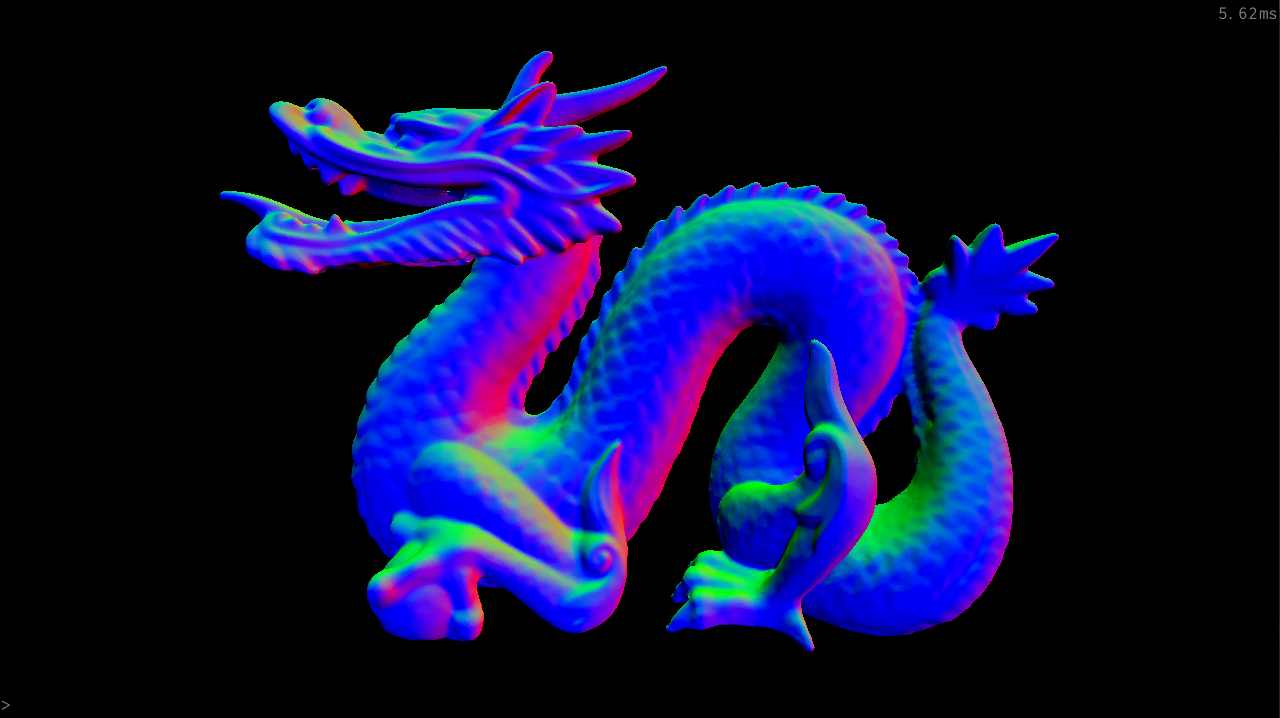
\includegraphics[scale=0.1,trim=0 0 0 -5]{img/results/g-buffer/normals-2layer-1} &
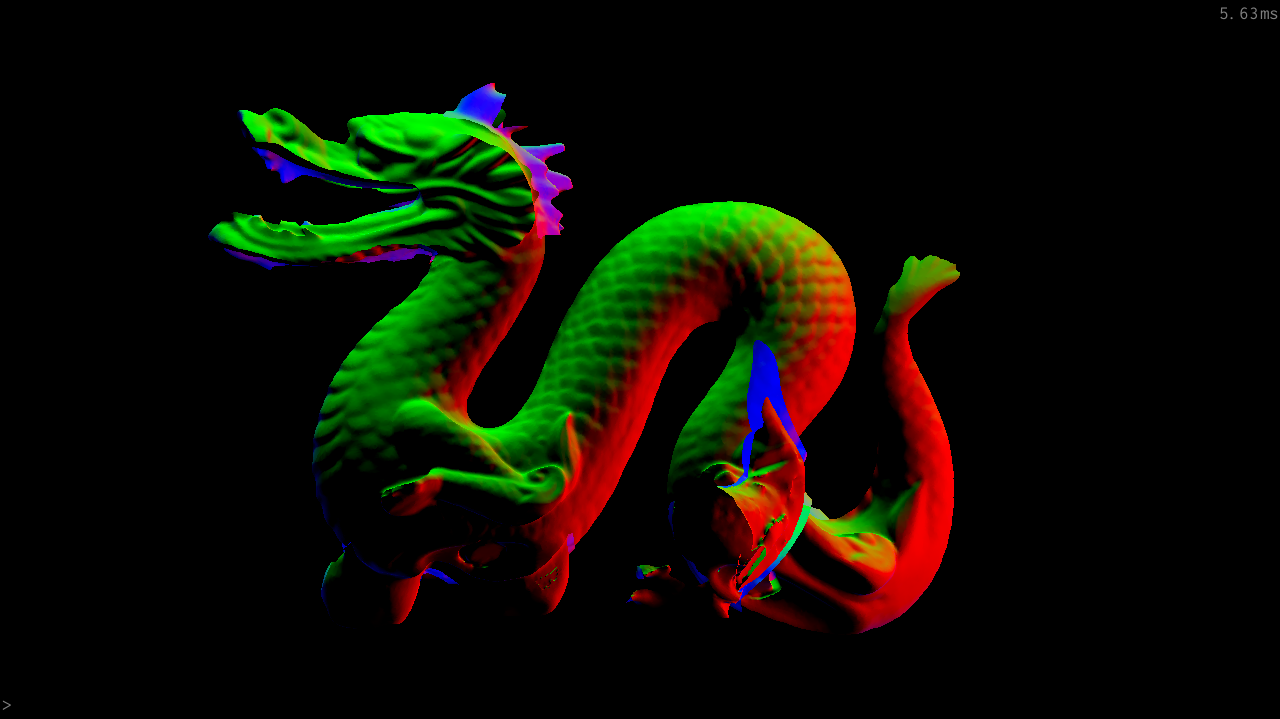
\includegraphics[scale=0.1,trim=0 0 0 -5]{img/results/g-buffer/normals-2layer-2} \\
\hline
\end{tabular}
\caption{Table with resulting Normal and Depth textures from the G-buffer generation.}
\label{table-buffers}
\end{table}

I also did a number of tests on the running time. One in which I rasterise two layers of geometry with the single-pass pipeline, and one in which only one layer is rasterised. I include a control result from the \emph{conference} scene for comparison to the double-layered result. These results can be seen in table \ref{table-gbuffer-time}.

\begin{table}[!ht]
\centering
\begin{tabular}{| c | p{2.5cm} | p{2.5cm} | p{2.5cm} |}
\hline
 & \emph{Dragon} 1 layer & \emph{Dragon} 2 layers & \emph{Conference} 2 layers\newline (Control) \\
\hline
\emph{Average Time} & 2.95ms & 5.62ms & 2.57ms \\
\hline
\end{tabular}
\caption{Table of G-buffer generation times.}
\label{table-gbuffer-time}
\end{table}

\subsection{Discussion}
For table \ref{table-buffers}, the resulting buffers are in line with what we would expect from the G-buffer generation. While it is hard to verify the depth-texture correctness, since it is stored in an exponential format and this appears mostly the same colour, we can tell by the results of the lambertian shader that the positions are, indeed correct. We can tell that the normals are correctly stored based on the colours shown. Since they are stored in view-space, we would expect front-facing fragments to appear blue as view-space coordinates have the camera oriented along negative Z. We'd expect increasingly red values for right-facing fragments and increasingly green values for upwards-facing fragments, which is exactly what we have.

The interesting thing about this test is the results shown in \ref{table-gbuffer-time}. For our single-pass generation pipeline, in which we transform geometry once in the vertex shader, we'd expect somewhat higher generation time for rasterising to two layers, but not almost doubled values. What this means is that the majority of time spent in rasterisation is spent on interpolation of vertices and normals rather than the transformations themselves. That said, the single-pass method is still superior to a potential double-pass one, since the double pass one would have to use two textures, which would be slower to read values from and would make for more messy code.

\section{Lambertian and Shadow Mapping}

\begin{table}[!ht]
\begin{center}
\begin{tabular}{| c | p{2.5cm} | p{2.5cm} | p{2.5cm} | p{2.5cm} |}
\hline
Model & \emph{Dragon} & \emph{Dragon} & \emph{Dragon} & \emph{Conference} \\
\hline
Rendering &
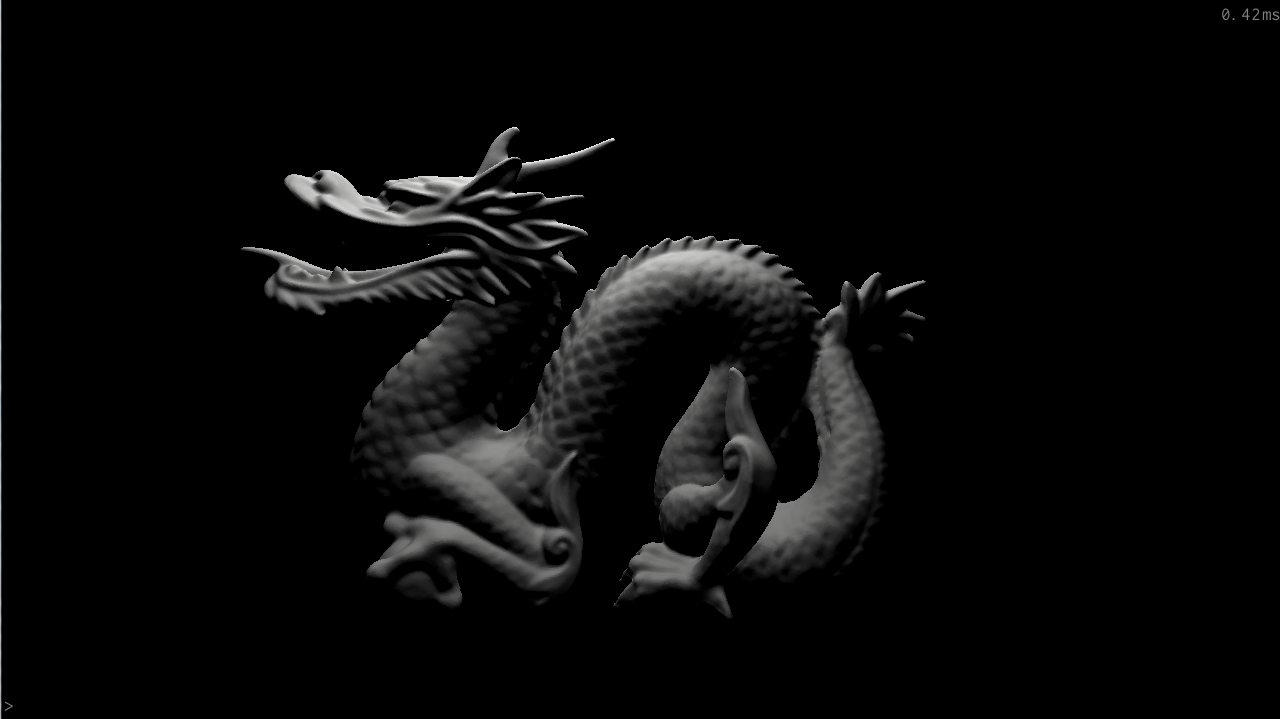
\includegraphics[scale=0.08,trim=0 0 0 -5]{img/results/lambertian/noocclusion-dragon} &
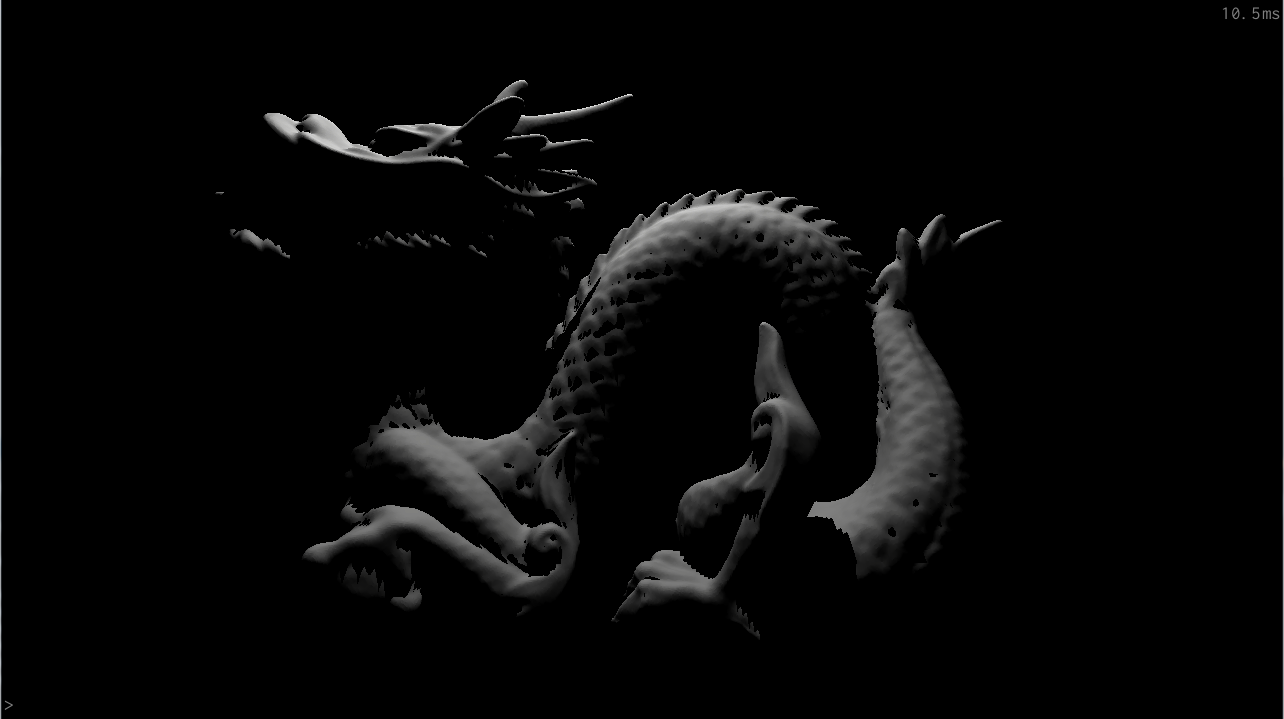
\includegraphics[scale=0.08,trim=0 0 0 -5]{img/results/shadowmap/480by480} &
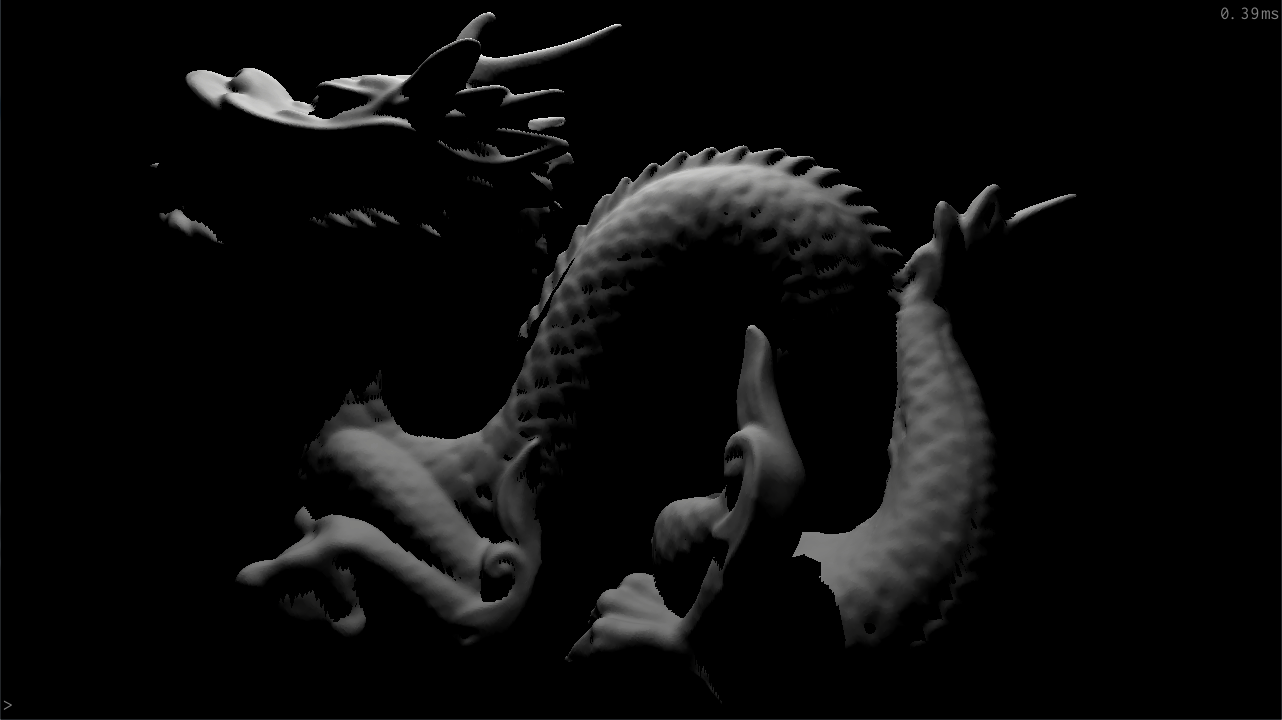
\includegraphics[scale=0.08,trim=0 0 0 -5]{img/results/lambertian/occlusion-dragon} &
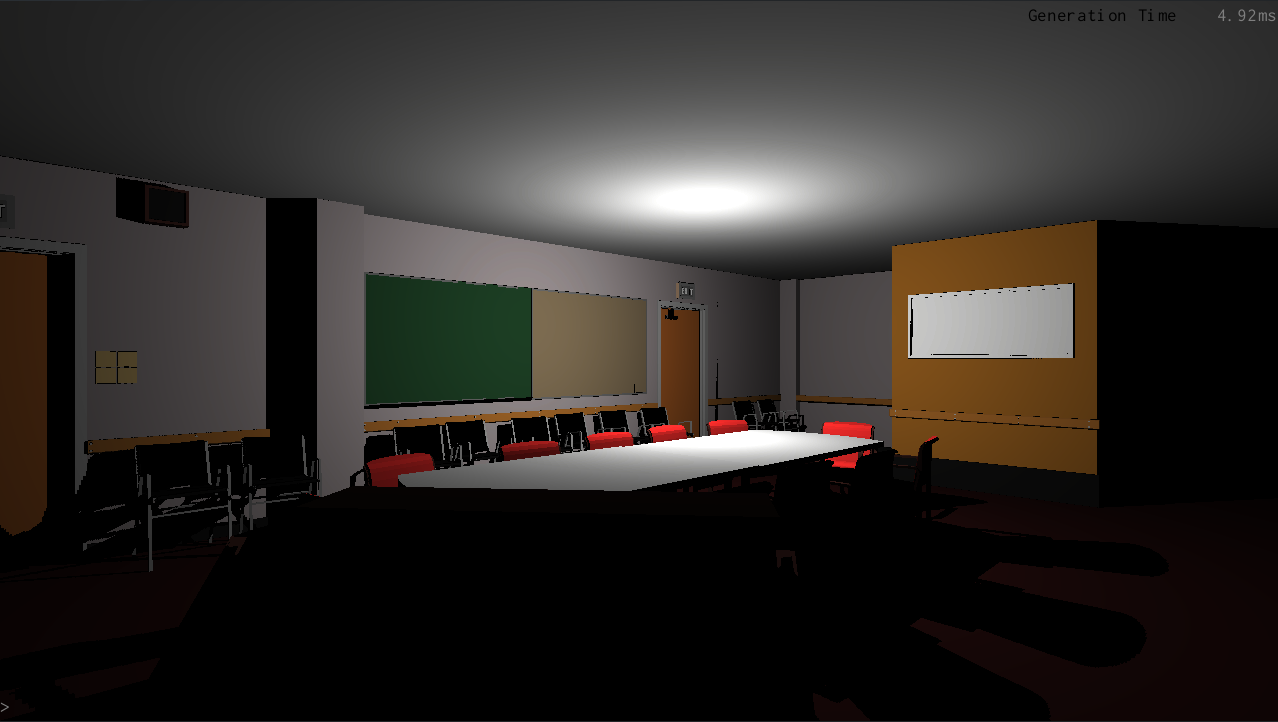
\includegraphics[scale=0.08,trim=0 0 0 -5]{img/results/shadowmap/conference1024x1024} \\
\hline 
\emph{Map Size} & No occlusion & 480 & 1024 & 1024\\
\hline
\emph{Lambertian Time} & 0.36ms & 0.36ms & 0.36ms & 0.36ms\\
\hline
\emph{Shadowmap Time} & 0.0ms & 10.4ms & 10.6ms & 4.90ms\\
\hline
\end{tabular}
\caption{Tests done on lambertian shading and shadow map generation. Shadowmap Time denotes the time spent to generate the shadow map.}
\label{table-lambert}
\end{center}
\end{table}

\subsection{Discussion}
A single run of the lambertian filter takes 0.36ms regardless of scene complexity and use of a shadow map. The independence from scene complexity is expected, since it is the primary feature of deferred rendering; however, the result being independent of use of a shadow map is unexpected. It is possible that the driver "guessed" that shadow mapping is going on and has done some optimisations to the shader behind the scenes. Alternatively my timer has somehow produced the wrong result. Whether or not to do scene reconstruction is a question of trading VRAM usage for performance. That said, 0.36ms to draw an occluded light source is a very reasonable result, considering we're doing per-fragment transformations and saving 64 bits of buffer space per fragment.

 I included the dragon model in the table because it demonstrates omni-directional shadow maps well. You can see that all objects in the scene are considered in the occlusion test, demonstrating that the shadow map works in all directions. As expected, the quality of the shadow increases between the 480x480 resolution per face to the 1024x1024 resolution per face, and luckily it has very little impact on performance. However, maintaining six 1024x1024 32-bit textures to test occlusion for a single light source is a big memory concern. The shadow map drawing time appears to be linearly dependent upon geometric complexity, which is also expected since we rasterise the scene to generate it. Spending 10ms on a single shadow map is infeasible for real-time applications if you wish to have time for other effects, and as such I would probably not recommend using this method unaltered. A possible alternative would be dual paraboloid shadow-maps which require only two textures, and thus only the geometry rasterised twice and has a third of the memory footprint. As a proof of concept, however, the cube shadowmap works as intended.

One final note is that there are some shadow artefacts (acne) on the dragon, and if you look closely at the corners of the conference room. It could be alleviated by adding more bias to the comparison, but adding any more bias causes peter panning in both the conference room and cornell box scenes. The current bias of $0.0001f$ was the best compromise between the two.

\section{Radiosity}
I use a sample radius of 300 to ensure that as large a part of screen-space as possible is covered, without losing too many samples by sampling outside of it. I also ensure that any value further away than 500 units is not considered part of the hemisphere, to maintain some enforcement of world-space consistency. Figure \ref{table-rad-samples} shows the consequence of changing the number of spiral taps done in the shader, while table \ref{table-rad-bounces} demonstrates the consequences of different different numbers of bounces. \ref{fig-rad-comparison} is the control in this case.

\begin{table}[!ht]
\begin{center}
\begin{tabular}{| c | p{3.5cm} | p{3.5cm} | p{3.5cm} |}
\hline
&
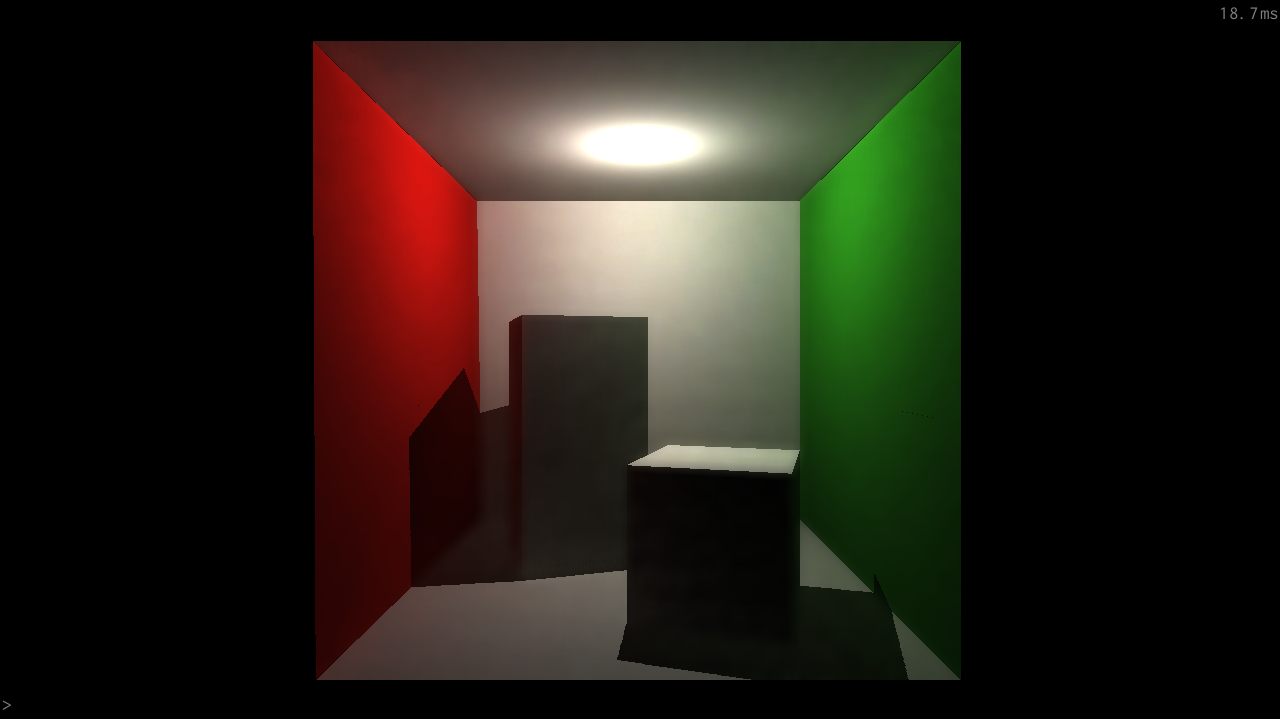
\includegraphics[scale=0.1,trim=0 0 0 -5]{img/results/radiosity/11samples} &
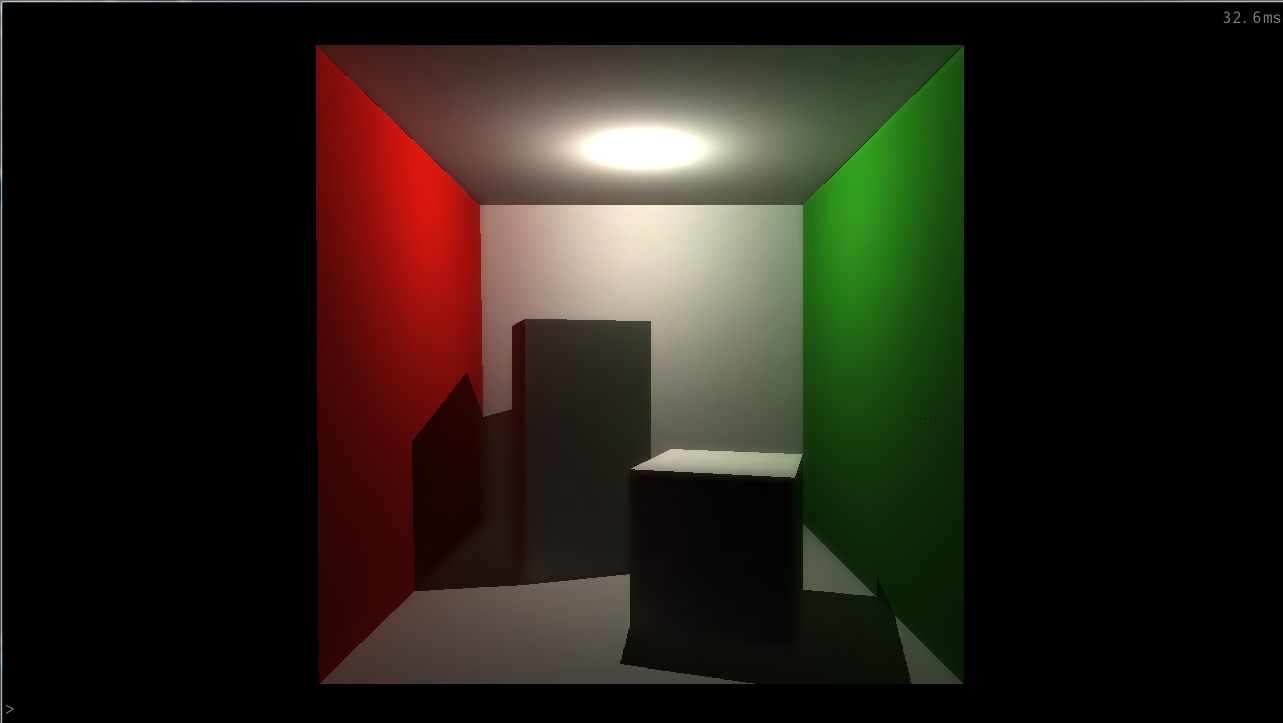
\includegraphics[scale=0.1,trim=0 0 0 -5]{img/results/radiosity/23samples} &
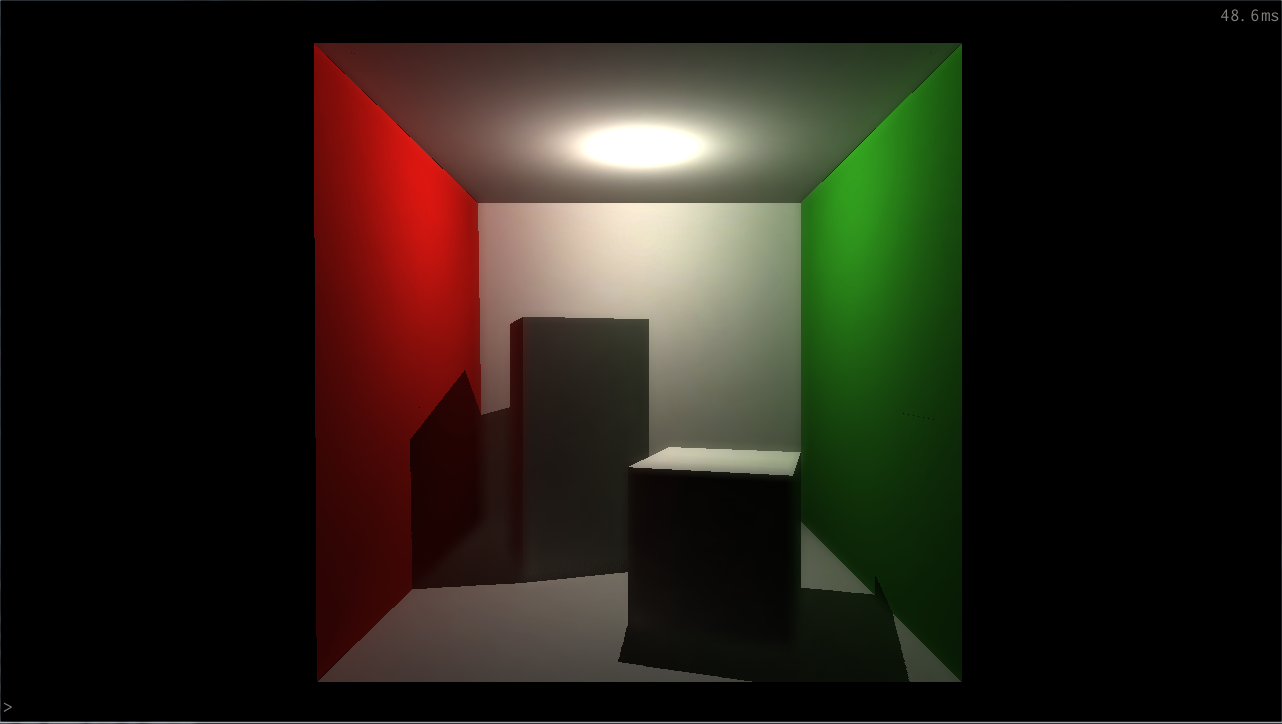
\includegraphics[scale=0.1,trim=0 0 0 -5]{img/results/radiosity/37samples} \\
\hline
\emph{Samples} & 11 & 23 & 37 \\
\hline
\emph{Frame Time} & 18.7ms & 32.6ms & 48.6ms\\
\hline
\end{tabular}
\caption{Table of frame times based on sample taps used to approximate radiosity. Time is for 2 bounces of radiosity.}
\label{table-rad-samples}
\end{center}
\end{table}

\begin{table}[!ht]
\begin{center}
\begin{tabular}{| c | p{3.5cm} | p{3.5cm} | p{3.5cm} |}
\hline
&
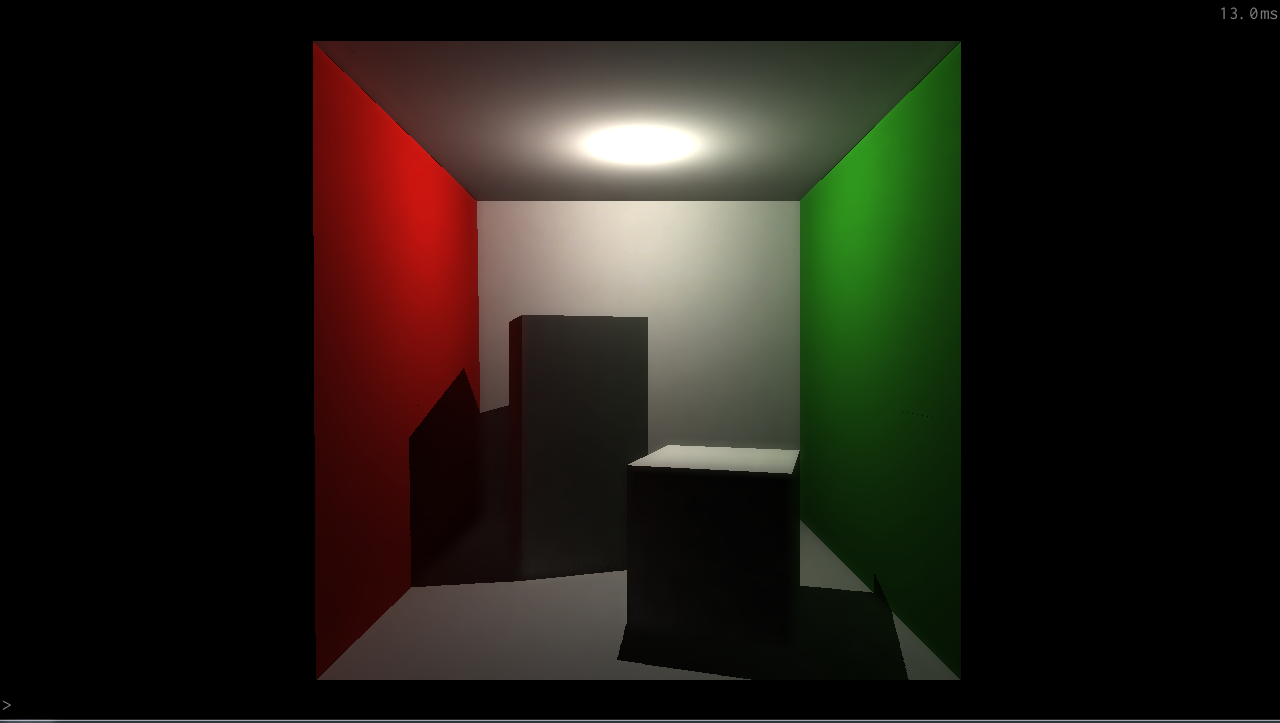
\includegraphics[scale=0.1,trim=0 0 0 -5]{img/results/radiosity/1bounce} &
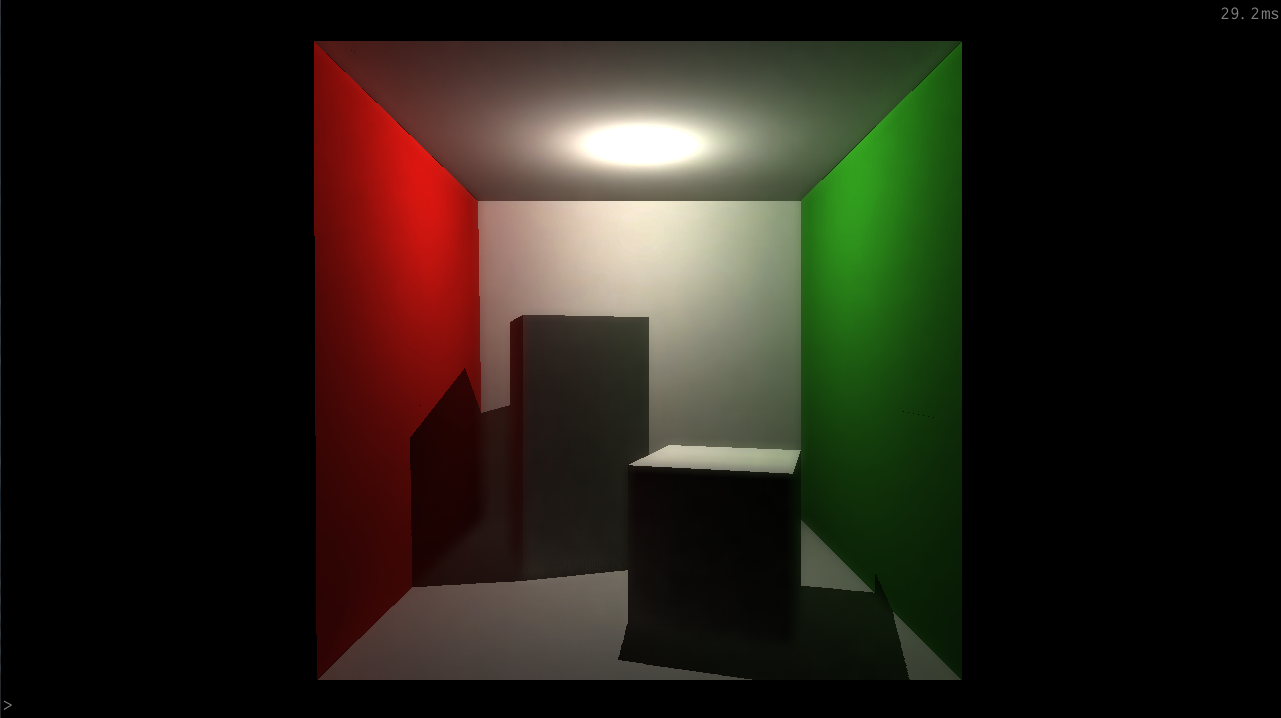
\includegraphics[scale=0.1,trim=0 0 0 -5]{img/results/radiosity/2bounce} &
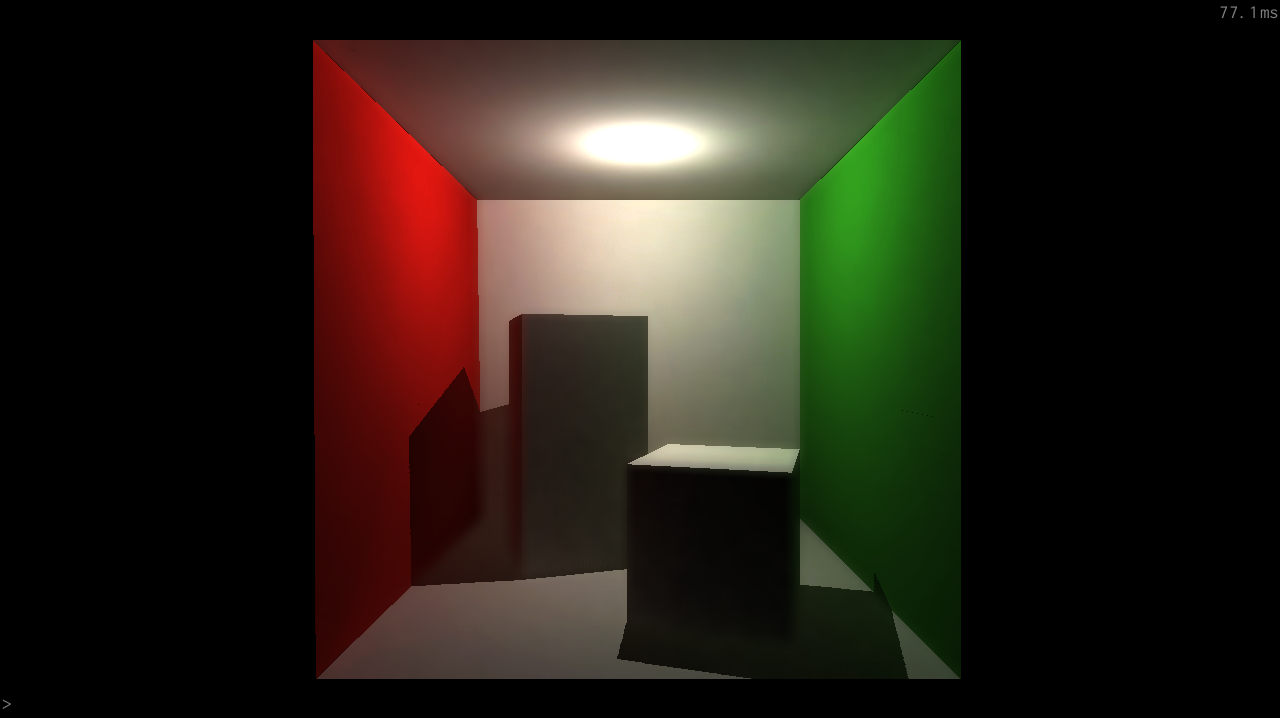
\includegraphics[scale=0.1,trim=0 0 0 -5]{img/results/radiosity/5bounce} \\
\hline
\emph{Bounces} & 1 & 2 & 5 \\
\hline
\emph{Frame Time} & 13.0ms & 29.1ms & 77.1ms\\
\hline
\end{tabular}
\caption{Table for the number of radiosity bounces used. Sample taps is 20.}
\label{table-rad-bounces}
\end{center}
\end{table}

\begin{figure}[!ht]
\centering
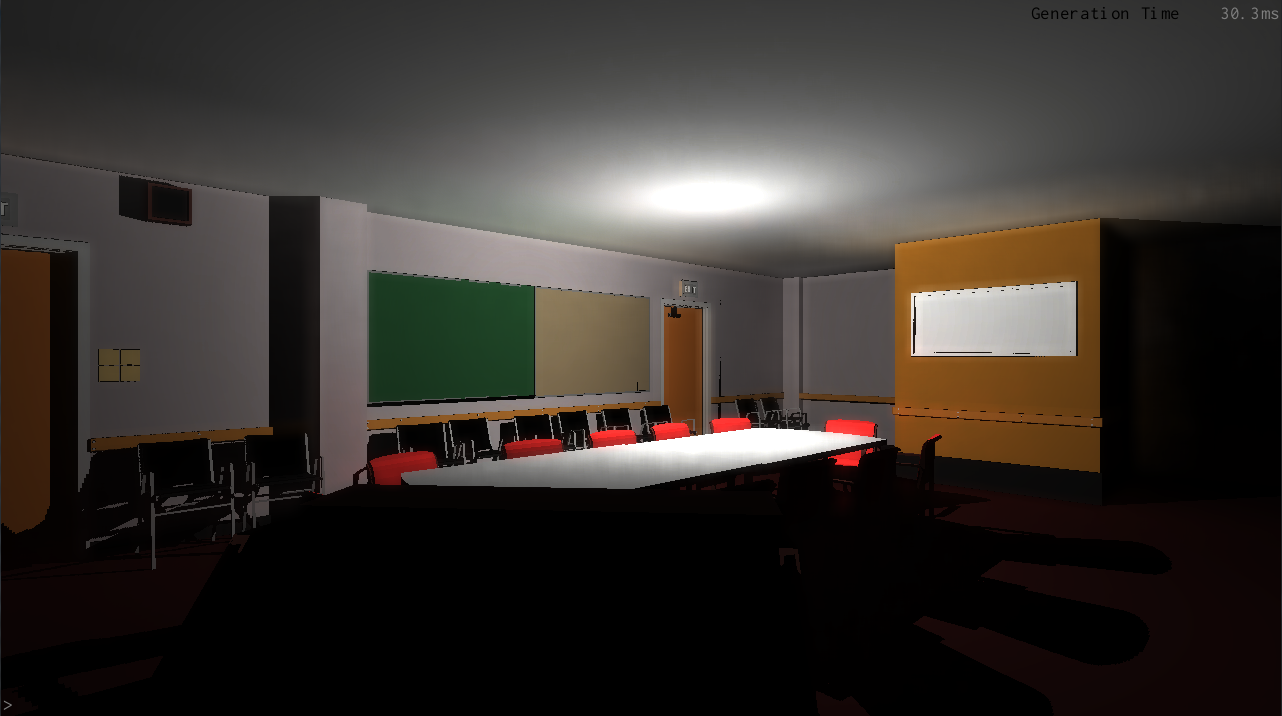
\includegraphics[scale=0.3]{img/results/radiosity/comparison}
\caption{Radiosity control scene (\emph{Conference}). 2 bounces, 23 samples. Time: 32.5ms}
\label{fig-rad-comparison}
\end{figure}

\subsection{Discussion}
Radiosity results look like expected, considering I'm not doing any occlusion testing. The red and green walls are bleeding unto the boxes, ceiling and floor, and the part of the room occluded by the large box is lit up. Rendering time rises linearly with the number of samples (seems to be around 1ms per sample.) As expected the result becomes smoother as the number of samples increases. For 11 samples, there's a lot of risidual noise from the randomisation, while it is mostly unnoticeable for 23 samples, and appears almost completely smooth for 37 samples. I would consider 23 samples an acceptable result, but 32.6ms is a \emph{lot} of time to spend on a single filter. However, this can be alleviated by implementing temporal filtering in which subsequent bounces are done in subsequent frames, and the result is filtered to account for the changing energy levels. Even with a single bounce of radiosity, though, the total time is 13ms or so, which is still a lot of time to be spending on a single effect.

For the number of bounces the time also seems to rise linearly with the number of bounces. It is a bit weird that the time more than doubles between bounce 1 and 2, but I consider that a measurement error of some nature. You can see the light propagating progressively from 1 to 5 bounces; for instance, the green and red contributions on the ceiling become increasingly noticeable, and the occluded spot behind the tall box becomes more and more illuminated. Radiosity seems to stop propagating after 4-5 bounces, which makes sense. Energy is lost with every bounce, and the textures used only allow for a certain amount of precision, meaning additions to the cumulating texture (containing all bounces and lambertian) become insignificant after a while.

\section{SSAO}

\begin{table}[!ht]
\begin{center}
\begin{tabular}{| c | p{3.5cm} | p{3.5cm} | p{3.5cm} |}
\hline
&
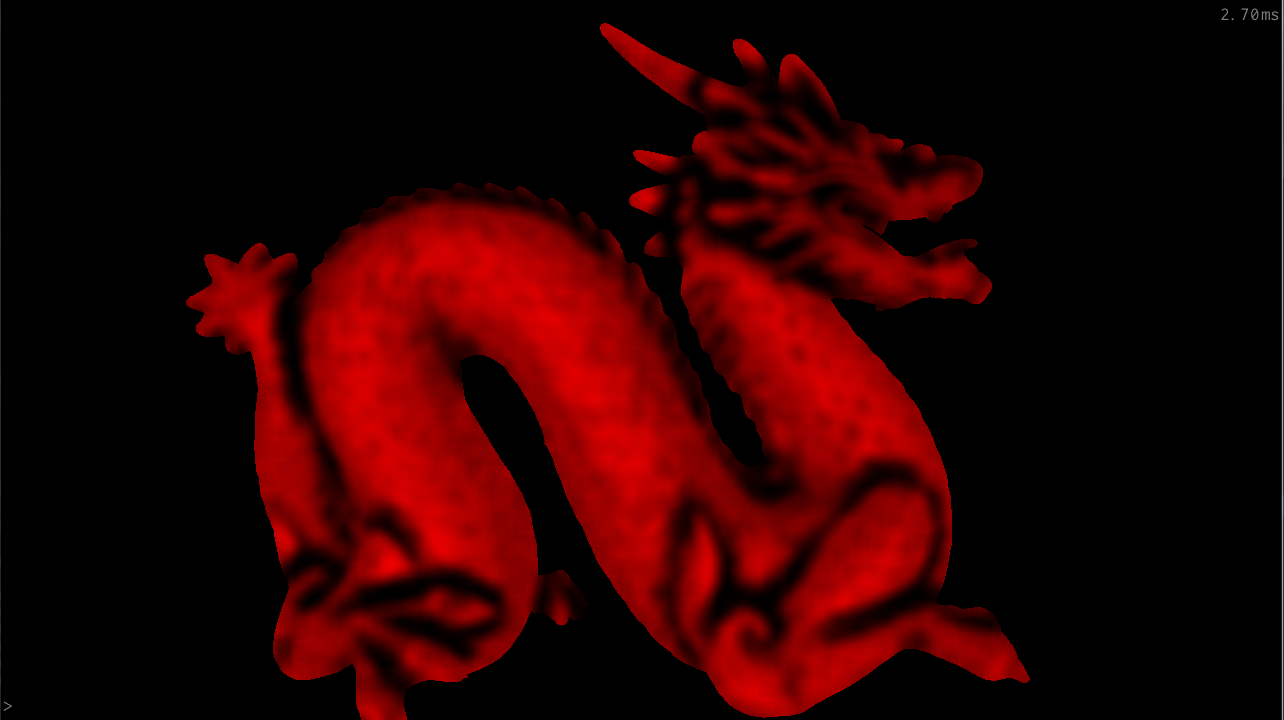
\includegraphics[scale=0.1,trim=0 0 0 -5]{img/results/ssao/11samplesdragon} &
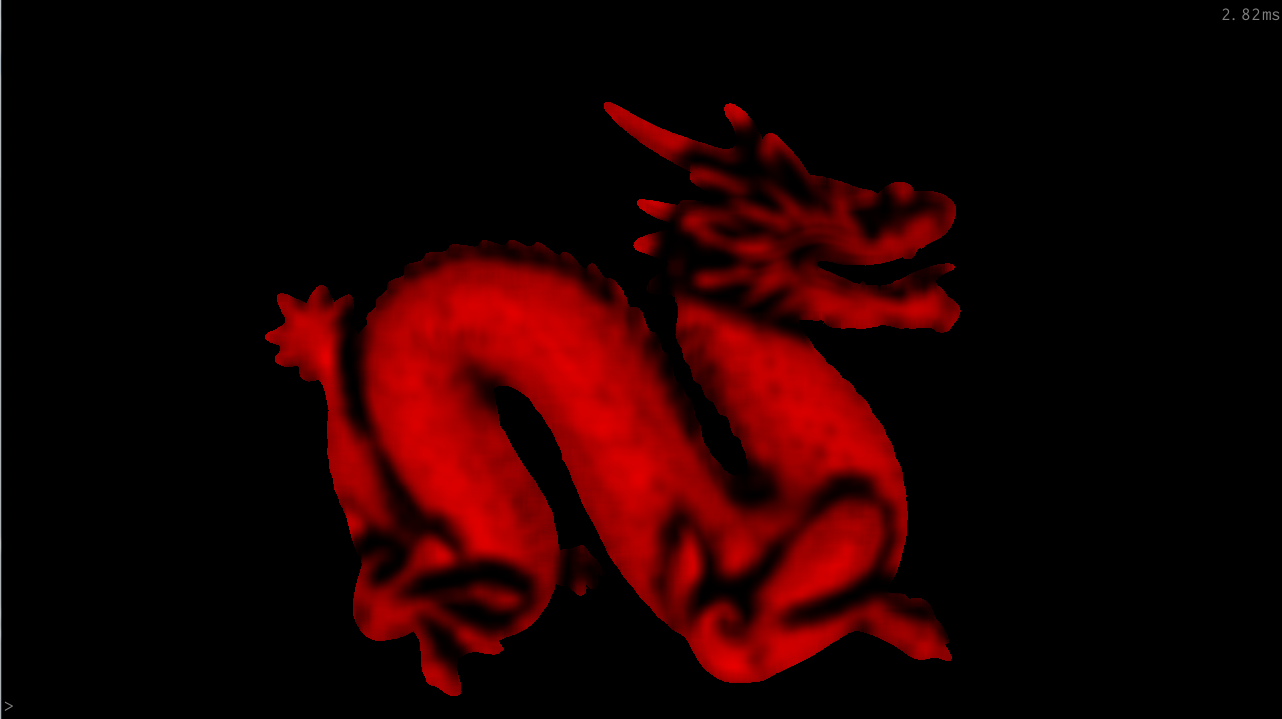
\includegraphics[scale=0.1,trim=0 0 0 -5]{img/results/ssao/23samplesdragon} &
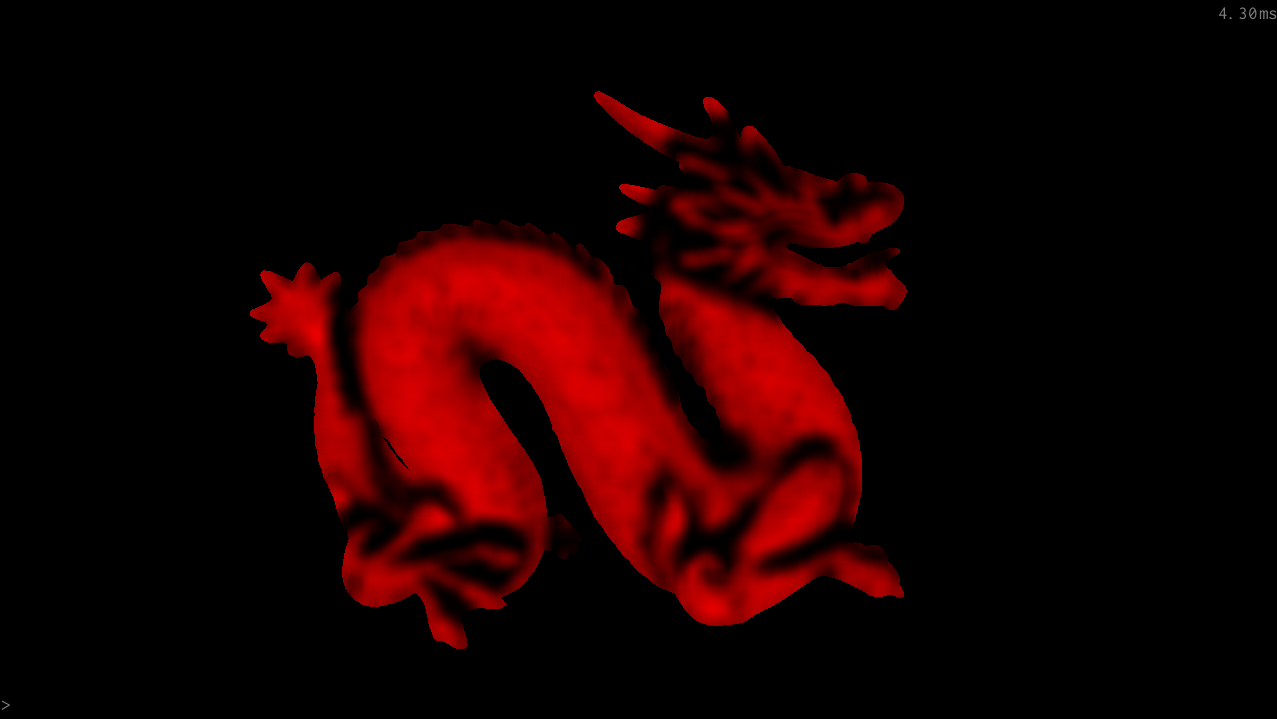
\includegraphics[scale=0.1,trim=0 0 0 -5]{img/results/ssao/37samplesdragon} \\
\hline
\emph{Samples} & 11 & 23 & 37 \\
\hline
\emph{Frame Time} & 2.71ms & 2.80ms & 3.17ms\\
\hline
\end{tabular}
\caption{Time to draw SSAO based on number of samples.}
\label{table-ssao-samples}
\end{center}
\end{table}

\subsection{Discussion}
The first thing I noticed is that there's very little difference in quality between the three sampling amounts, but I would consider them all acceptable. However, what's interesting to note is that there's very little difference in filtering time across the three levels. Additionally, the time taken is significantly lower than that of radiosity. There could be a number of reasons for this; either the texture is stored in such a way that adjacent values are faster to read than values that are far from each other. Since SSAO uses a scree-space sampling radius of around 30 and radiosity's is 300, if this were the case, it would explain the big difference. The other is that the \verb=R11F_G11F_B10F= textures used for radiosity, and the fact that radiosity has blending as well, creates so much overhead that the shader runs much slower than it could've if the texture formats were more appropriate. Using more textures to generate the radiosity result probably also contributes to this. This is in accordance with the finding that changing the normal texture to \verb=GL_RGB16F= actually improved performance on all filters by quite a bit.

Since SSAO is a one-time filter per frame, 2-3ms isn't too bad considering the results it produces.

\section{Gaussian Filter}

\begin{table}[!ht]
\begin{center}
\begin{tabular}{| c | p{5cm} | p{5cm} |}
\hline
&
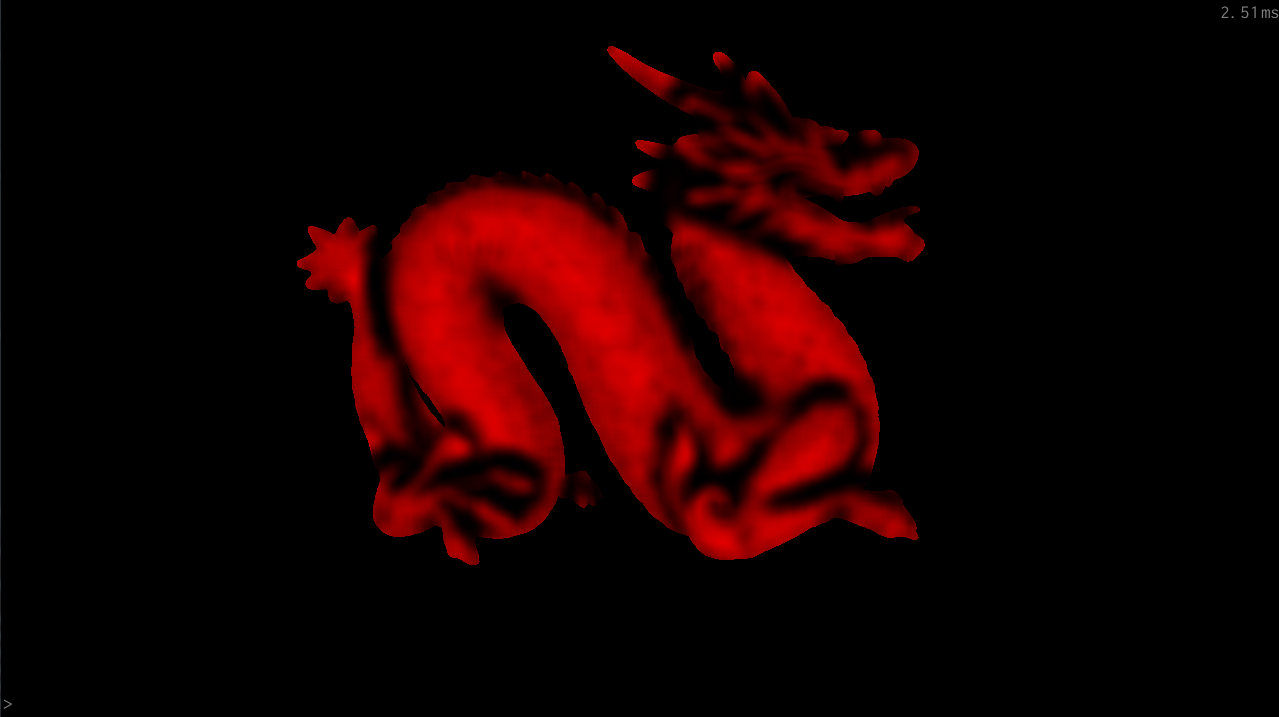
\includegraphics[scale=0.15,trim=0 0 0 -5]{img//results/ssao/dragon-gauss} &
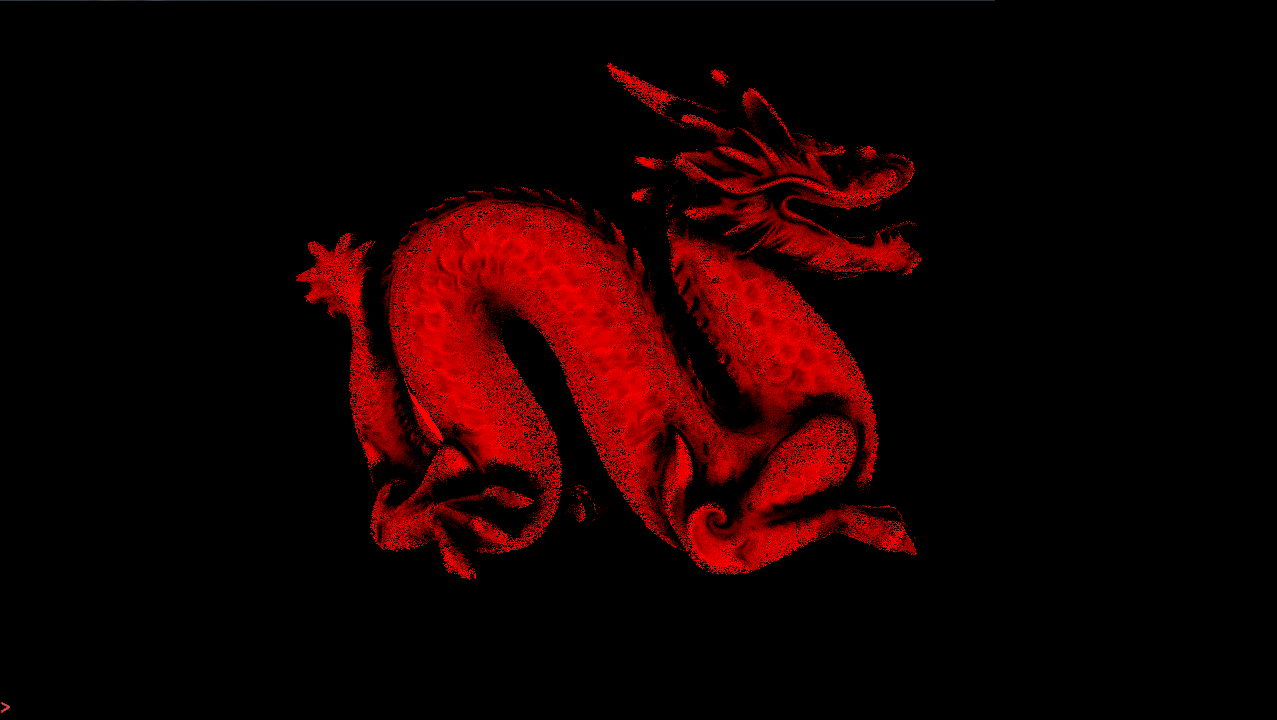
\includegraphics[scale=0.15,trim=0 0 0 -5]{img/results/ssao/dragon-nogauss} \\
\hline
\emph{Filtered} & Yes & No \\
\hline
\emph{Frame Time} & 2.50ms & 1.61ms \\
\hline
\end{tabular}
\caption{Gussian filtering on SSAO. Radius = 20}
\label{table-gauss-ssao}
\end{center}
\end{table}

\begin{table}[!ht]
\begin{center}
\begin{tabular}{| c | p{5cm} | p{5cm} |}
\hline
&
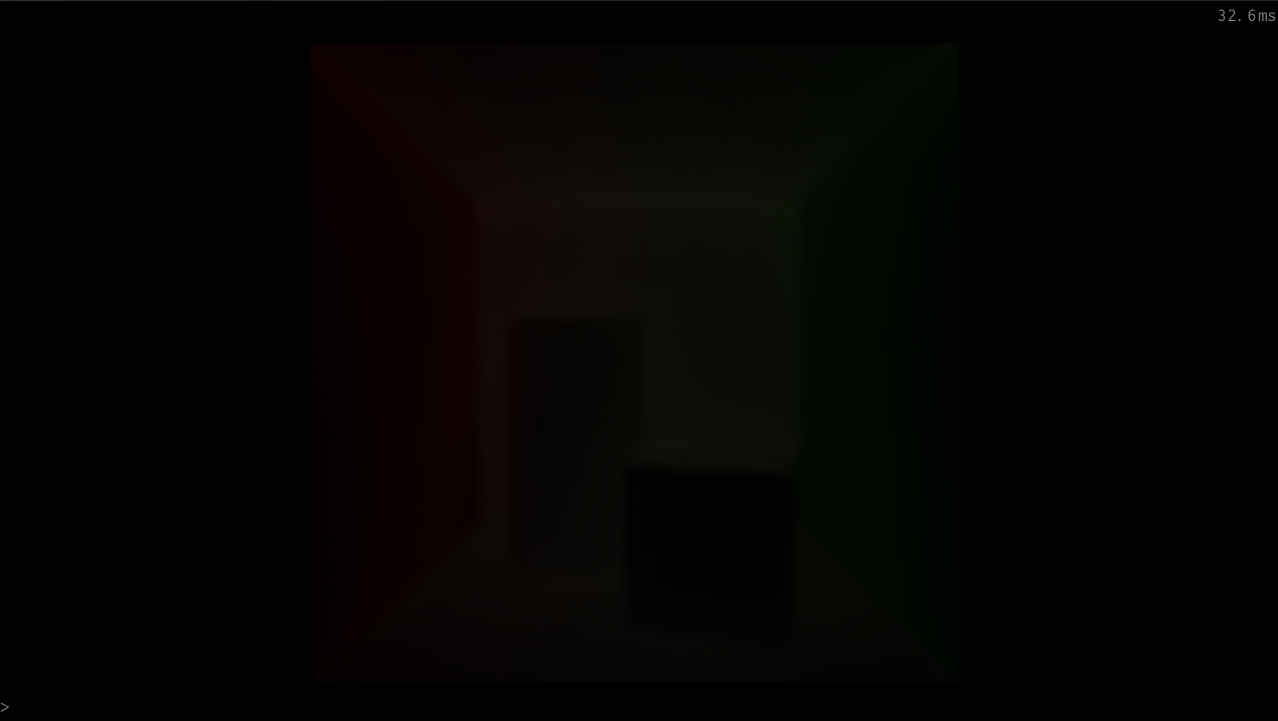
\includegraphics[scale=0.15,trim=0 0 0 -5]{img//results/radiosity/wBlend} &
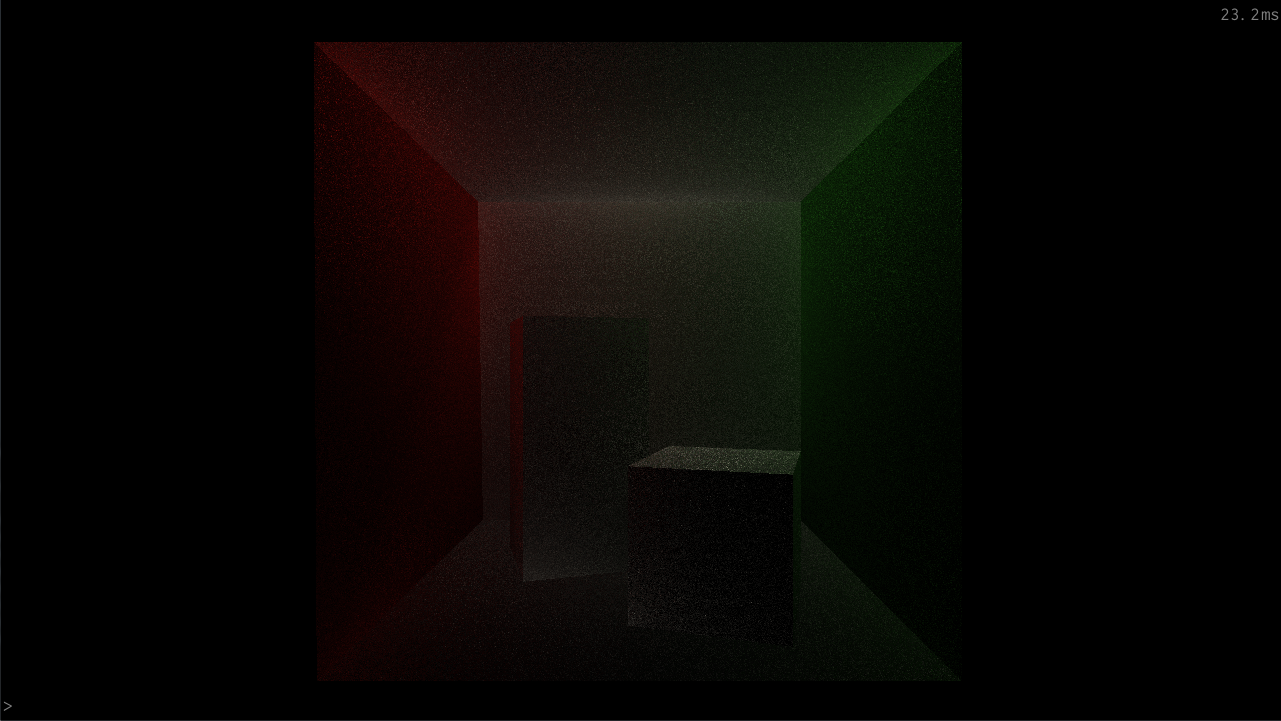
\includegraphics[scale=0.15,trim=0 0 0 -5]{img/results/radiosity/woBlend} \\
\hline
\emph{Filtered} & Yes & No \\
\hline
\emph{Frame Time} & 32.6ms & 23.2ms \\
\hline
\end{tabular}
\caption{Gussian filtering on Radiosity bounce. Gauss radius = 20, 2 bounces, 23 samples.}
\label{table-gauss-rad}
\end{center}
\end{table}

\subsection{Discussion}
The benefit of applying the modified Gaussian filter is immediately visible for both radiosity and SSAO. For a high enough radius (I found 20 to be the best balance,) the random noise is almost completely unnoticeable. You can tell on the right hand side that there are a lot of black spots on the SSAO result, and high variance on the radiosity result, which are both entirely gone after the filter has been applied. One weird thing, though, is the fact that filtering the SSAO only adds .89ms to the time, whereas filtering the radiosity adds around 4ms per frame. This is the primary reason I think the high rendering times on the radiosity filter is caused by one of the choices I made in regards to texture formats and blending, since the Gaussian filters for the two are identical except for those two facts.

Another thing to note is that while the depth-based edge-aware filter does alleviate some bleeding between surfaces that are at different depths, surfaces with different normals still bleed into each other, creating blurry results around edges of the same object. A way to alleviate this in an efficient manner would be to run an edge-detection filter that could be used by all Gaussian filters. It would hold a single float of value 0 or 1, which would be determined by some factor of depth and the normal's relation to surrounding normals. When the Gaussian filter hits whatever value we say is the edge value (probably a 1 for positive,) it would stop taking contributions in that direction. It does mean we would have to loop through the source texture from the center, in stead of from -radius to radius, but that is a minor fix.

As it is, considering the efficiency of the filter in smoothing out results, I'd consider 0.9ms a reasonable time for the result it gives.

\section{Composite Rendering}
The following table contains composite renderings of all three scenes with one layer and two layers. The composite is the sum of radiosity, and SSAO multiplied by ambient reflectance.

\begin{table}[!ht]
\begin{center}
\begin{tabular}{| c | p{3.5cm} | p{3.5cm} | p{3.5cm} |}
\hline
\emph{Model} & \emph{Dragon} & \emph{Cornell} & \emph{Conference} \\
\hline
\multicolumn{4}{|c|}{\emph{One Layer}} \\
\hline
\emph{Rendering} &
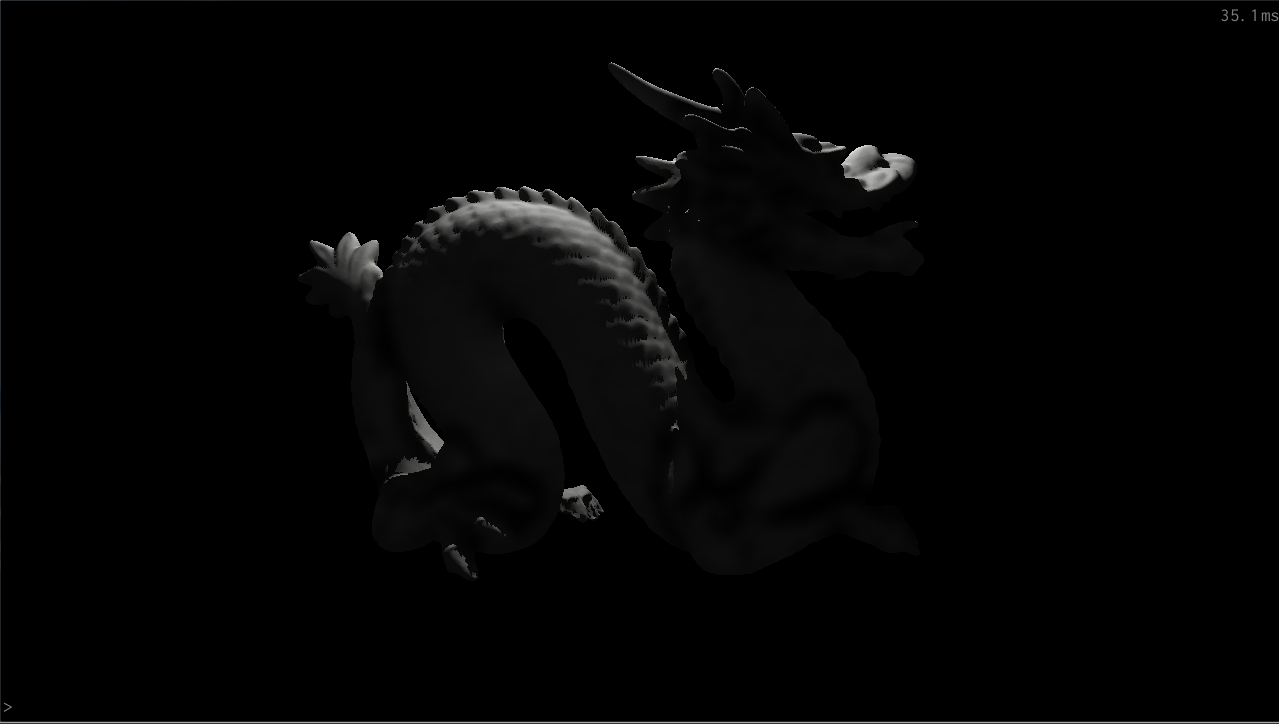
\includegraphics[scale=0.1,trim=0 0 0 -5]{img/results/composite/dragon-1layer} &
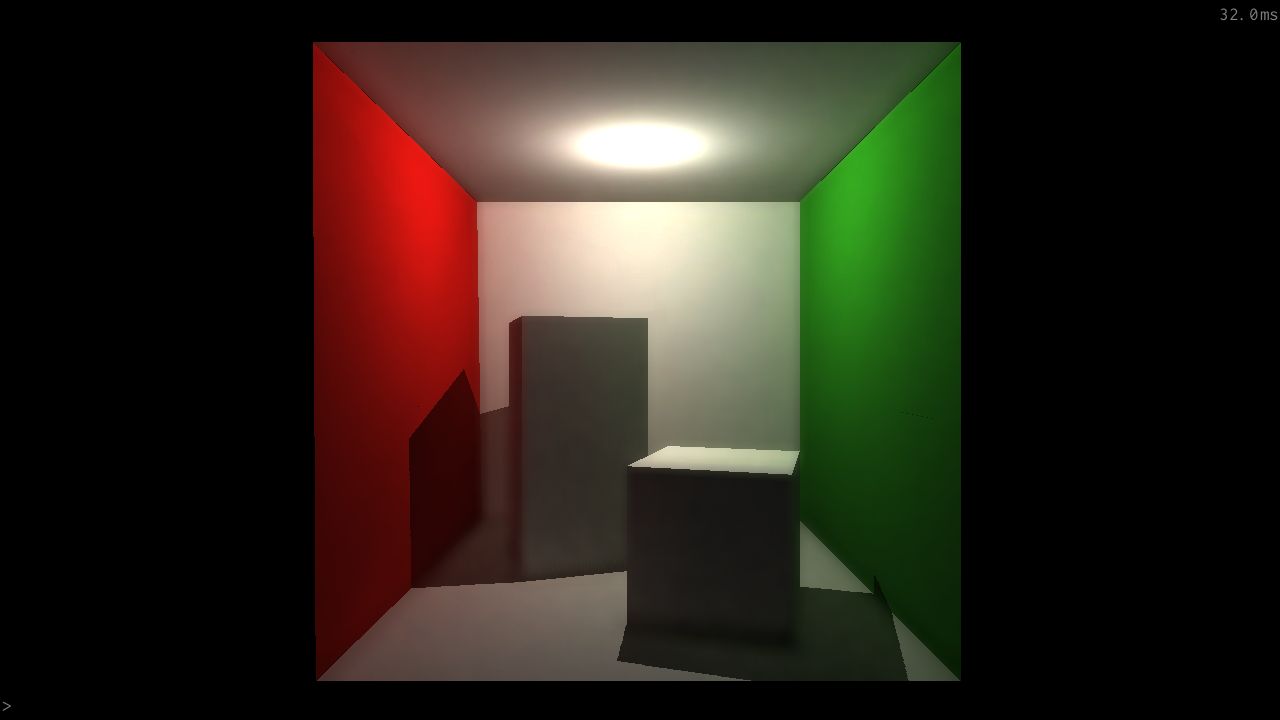
\includegraphics[scale=0.1,trim=0 0 0 -5]{img/results/composite/cornell-1layer} &
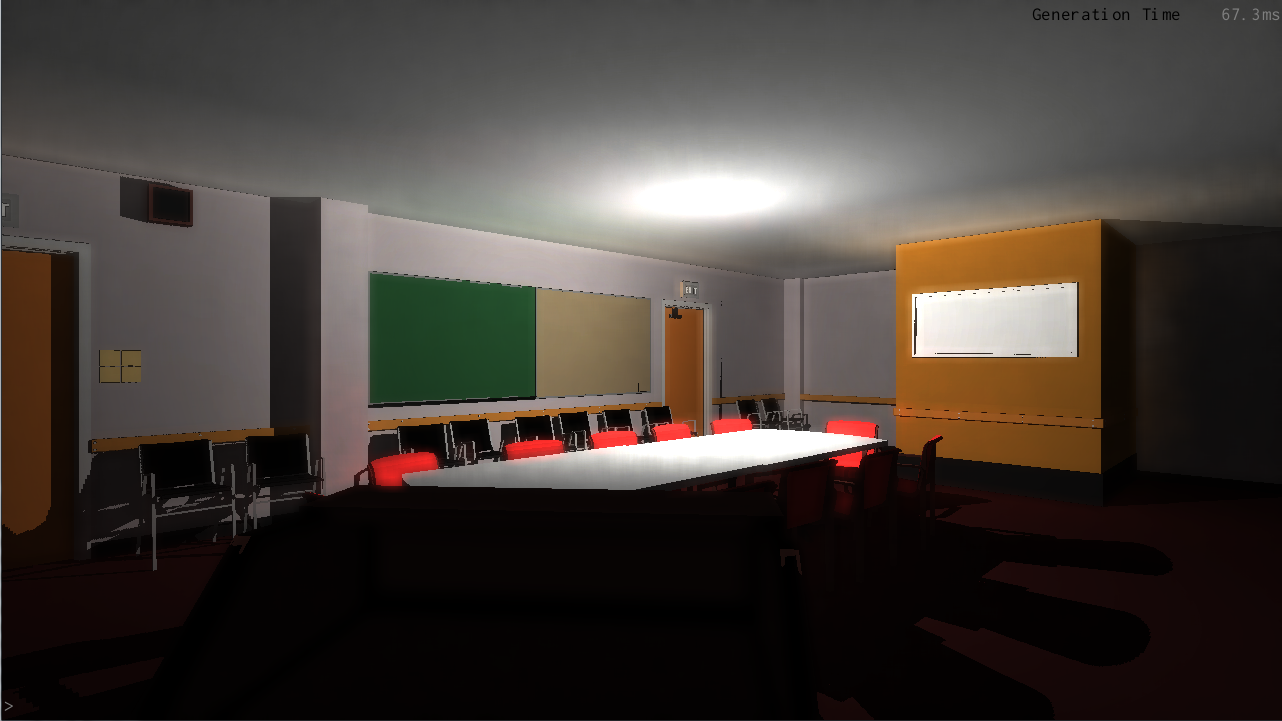
\includegraphics[scale=0.1,trim=0 0 0 -5]{img/results/composite/conference-1layer} \\
\hline
\emph{Frame Time} & 35.0ms & 43.0ms & 67.3ms\\
\hline
\multicolumn{4}{|c|}{\emph{Two Layers}} \\
\hline
\emph{Rendering} &
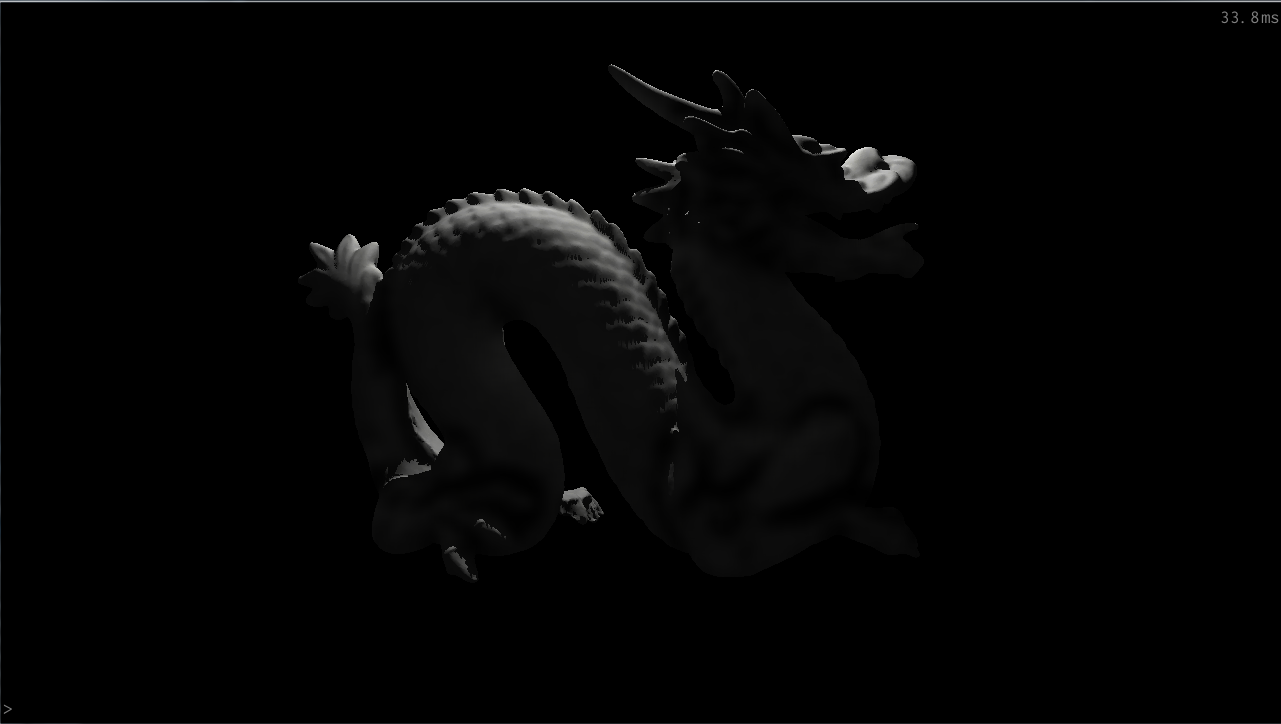
\includegraphics[scale=0.1,trim=0 0 0 -5]{img/results/composite/dragon-2layer} &
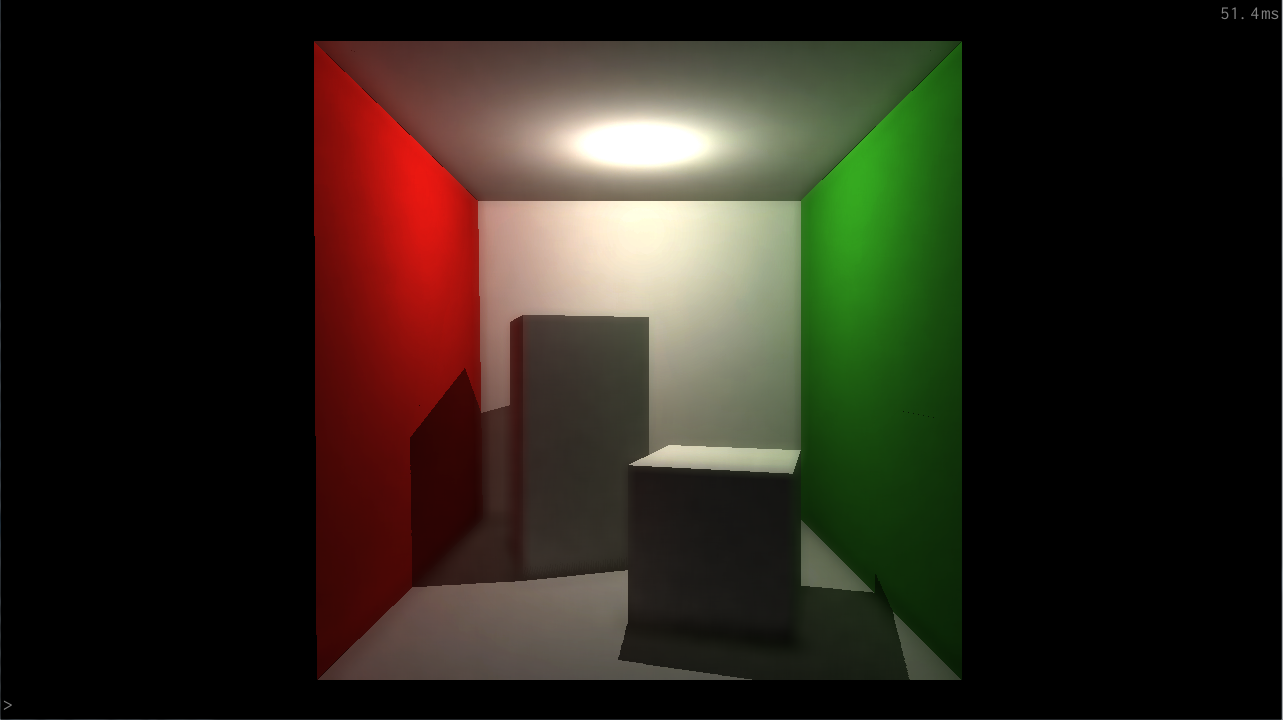
\includegraphics[scale=0.1,trim=0 0 0 -5]{img/results/composite/cornell-2layers} &
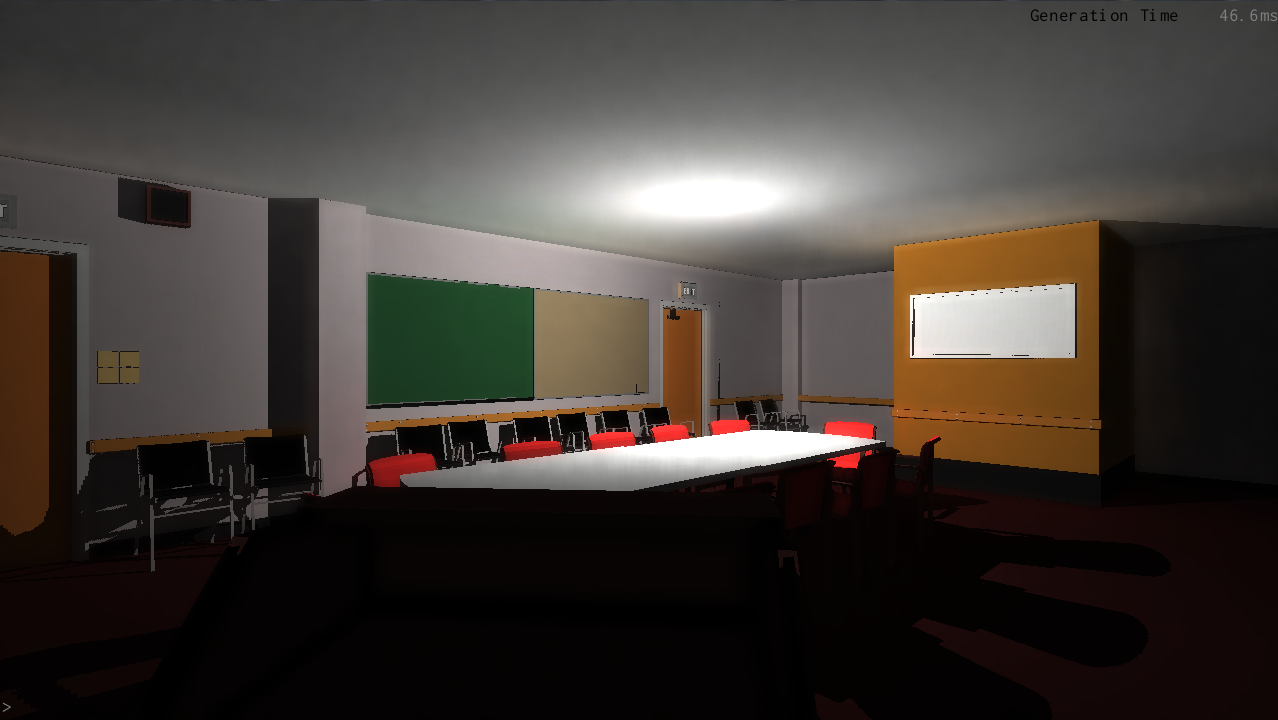
\includegraphics[scale=0.1,trim=0 0 0 -5]{img/results/composite/conference-2layer} \\
\hline
\emph{Frame Time} & 55.6ms & 51.4ms & 50.6ms\\
\hline
\end{tabular}
\caption{Time to draw the final scene with one or two layers of G-buffer. Samples = 23, Radiosity bounces = 1.}
\label{table-final}
\end{center}
\end{table}

\subsection{Discussion}
My first thought here is that there's no noticeable difference between one-layered and two-layered rendering in terms of the final output. There are some minor differences, where you can see some slight contribution from a surface hiding behind another. This is primarily caused, however, by the choice in scenes. These are all geometrically simple scenes, in the sense that there isn't a lot of geometric variation. This also means that the purpose of the deep G-buffer is lost. \ref{table-provingapoint} demonstrates one case in which the deep G-buffer is an advantage, since you can see green contribution on the ceiling from the chalkboard occluded by the chair. That in mind, however, the advantages presented by the deep G-buffer do not, in my opinion, justify the additional costs documented throughout this chapter. Luckily, however, there are multiple ways in which to improve performance. First of all, changing the shadow-map to a cheaper method with two planes in stead of one using dual paraboloid shadow mapping. Secondly, changing the radiosity render targets to a more efficient format and looking for other reasons why it might run that much slower than the SSAO filter. It would also be an option to look into the gaussian filter to maybe only sample every other fragment in the source texture, to cover the same area with less samples, at the cost of filtering quality. Obviously, it would be a good idea to look into the G-buffer generation to figure out why the single-pass generation still doubled the generation time, since it would be an ideal place to look for performance improvements.

\begin{table}[!ht]
\begin{center}
\begin{tabular}{| c | p{5cm} | p{5cm} |}
\hline
&
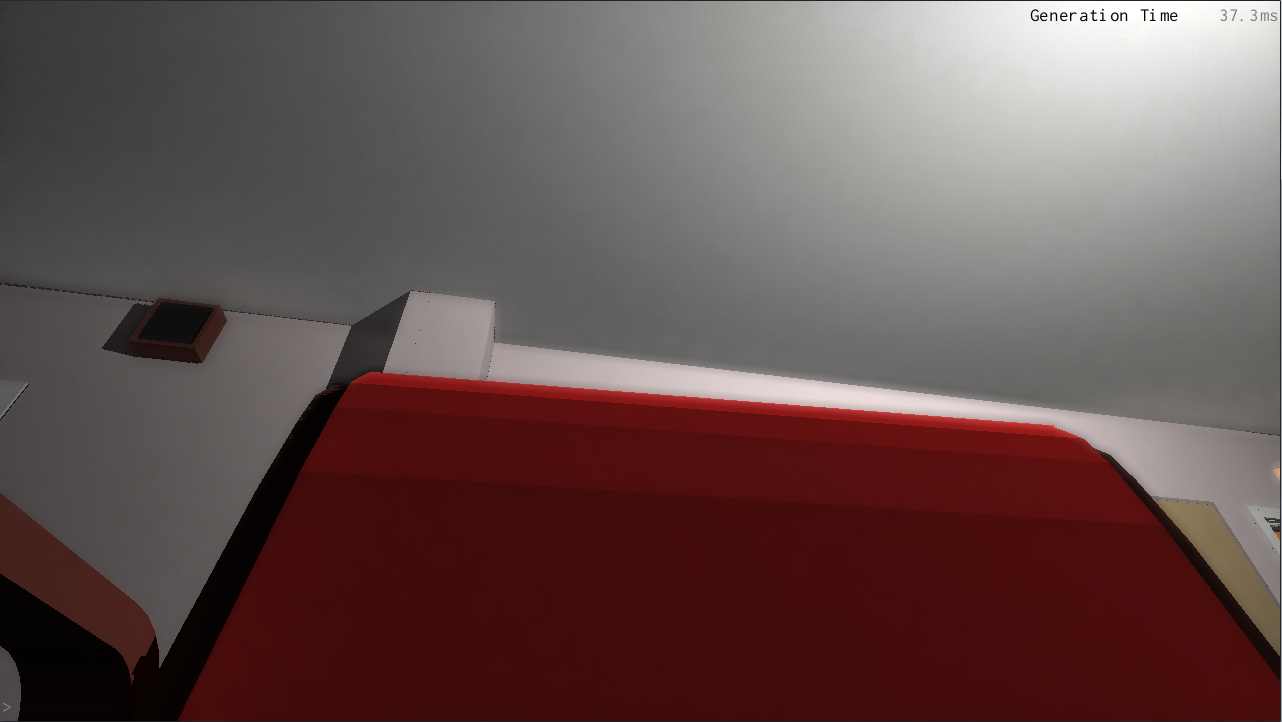
\includegraphics[scale=0.15,trim=0 0 0 -5]{img//results/various/1layer-rad} &
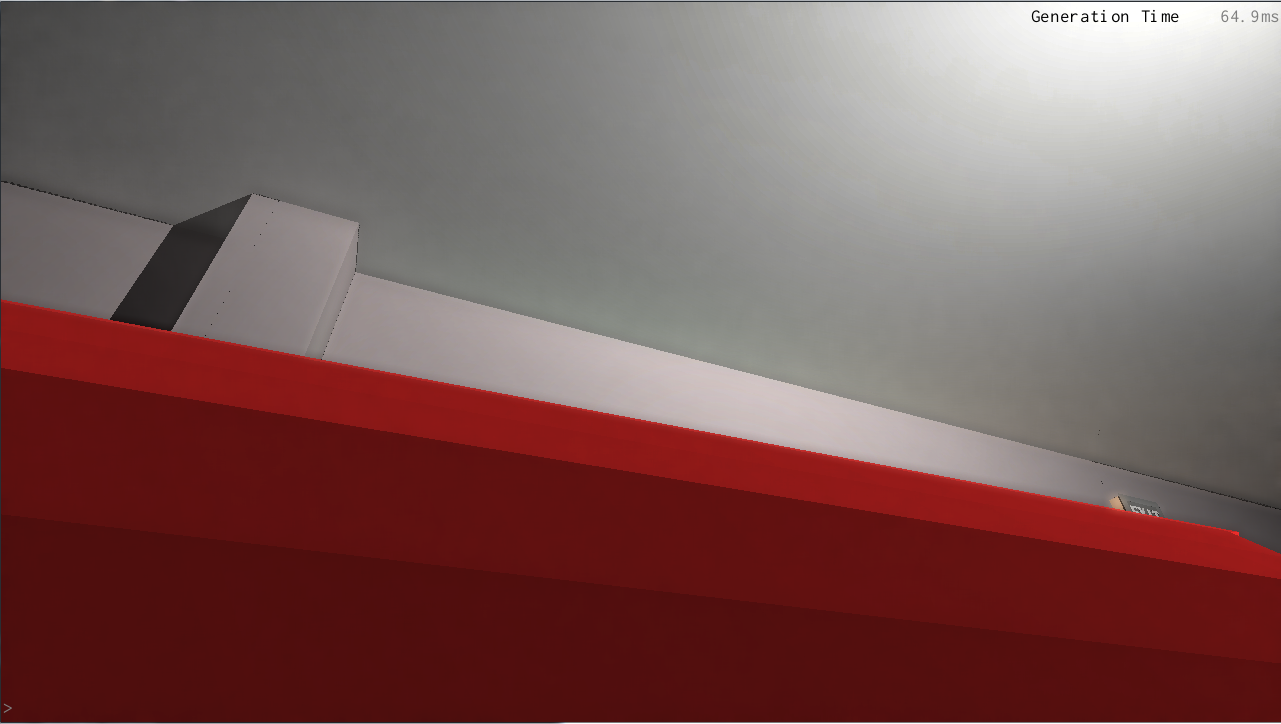
\includegraphics[scale=0.15,trim=0 0 0 -5]{img/results/various/2layer-rad} \\
\hline
\emph{Layers} & 1 & 2 \\
\hline
\end{tabular}
\caption{Demonstrating advantage of deep G-buffer.}
\label{table-provingapoint}
\end{center}
\end{table}

In general, the final product of this thesis demonstrated the concepts of screen-space radiosity, recostruction of positions from a depth buffer, SSAO and omni-directional shadow mapping, it failed to prove the advantage of a deep G-buffer. The costs of it, both in terms of memory and performance, simply turned out to not be worth the benefit. However, a lot of the problems appear to be fixable with optimisations, and I would consider it a reasonable claim that with optimisations and temporal filtering for multiple radiosity bounces, it would be possible to get very reasonable frame times. We're already very close to frame-times that would be considered acceptable for interactive applications, 50ms or 20FPS. Also, the conclusion that I did not prove the usefulness of a deep G-buffer is also influenced by the choice in scenes; different scenes may lead to other conclusions. Of course, the pipeline still has the problem that anything that escapes the viewing frustum will lose its impact on the scene, which is a problem that will persist regardless of scene due to the nature of deferred rendering.
%\chapter{Discussion}
\chapter{Conclusion}
Throughout this thesis I have documented the theory and implementation of a deep G-buffer and its use for two different kinds of global illumination techniques. Additionally, I have documented and implemented an omni-directional shadow map for use with a point light as well as reconstruction of view-space and world-space positions from a single G-buffer. I started by describing the basic idea of deferred rendering before moving on to the deep G-buffer and how to reconstruct positions from a depth buffer with the use of inverse matrices. Then I described the generation and use of an omni-directional shadow map based on a cubemap, after which I described radiosity, taking a point of departure in the rendering equation and using the patch method as a point of reference. I explained the screen-space method and the Quasi-Monte Carlo method used to approximate the radiosity equation. Finally I described the Alchemy AO equation and the Gaussian filter used to even out the noisy results of radiosity and SSAO. I used the concepts described in the theory chapter to implement a rendering pipeline, and documented the code in the implementation chapter. Finally, I posted screen shots and frame times of my results and drew my conclusions. Firstly, I conclude that generating the G-buffer in a single pass was the superior approach compared to multiple passes, both in terms of efficiency and code readability. I concluded that the scene reconstruction provided a reasonable time for a lambertian shader for the memory it saves, but the shadow map generation was too inefficient to be practical, despite producing nice results. I moved on to the radiosity and SSAO results and concluded that while radiosity was too expensive in running time per bounce, the SSAO algorithm ran within an acceptable time frame. For the Gaussian filter I concluded that, while it needs some more refined edge detection, it smooths the results out appropriately. Ultimately I concluded that I have not demonstrated the advantages of a G-buffer to a satisfactory degree, and would not consider it worth the extra running time on my system. I note, however, that the combined running times are very close to 20FPS, which is a fair goal for an interactive application. However, I successfully explained, implemented and demonstrated screen-space radiosity, SSAO, a gaussian filter and omni-directional shadow mapping, and conclude that with some optimisations the final running times could be brought down to acceptable levels.
\begin{thebibliography}{9}

\bibitem{radiosity}
  Philip Willis,\\
  \emph{Advanced Computer Graphics},\\
  Chapter 5: Radiosity Rendering\\
  Retrieved on: 13/12 2015 from\\
  \url{http://www.cs.bath.ac.uk/~pjw/NOTES/75-ACG/ch5-radiosity.pdf}
  

\bibitem{deep-g-buffer}

  Michael Mara and Morgan McGuire and Derek Nowrouzezahrai  and David Luebke,\\
  \emph{Fast Global Illumination Approximations on Deep G-Buffers},\\
  16/6 2014,\\
  NVIDIA Corporation,\\
  \url{http://graphics.cs.williams.edu/papers/DeepGBuffer14}
  
\bibitem{deferred}
	Shawn Hargreaves and Mark Harris,\\
	Deferred Shading \\
	Retrieved on: 17/12 2015,\\
	NVIDIA Corporation,\\
	\url{ftp://download.nvidia.com/developer/presentations/2004/6800_Leagues/6800_Leagues_Deferred_Shading.pdf}

\bibitem{bilat}
	Sylvain Paris, Pierre Kornprobst, Jack Tumblin, and Frédo Durand,\\
	\emph{An Easy Introduction to Bilateral Filtering and Its Applications},\\
	Massechussets Institute of Technology,\\
	Retrieved on: 19/12 2015,\\
	\url{http://people.csail.mit.edu/sparis/bf_course/}
	
\bibitem{cubetex}
	OpenGL/Khronos Foundation.\\
	\emph{Cubemap Texture}\\
	\url{https://www.opengl.org/wiki/Cubemap_Texture}
	
\bibitem{VV11AlchemyAO}
  Morgan McGuire and Brian Osman and Michael Bukowski and Padraic Hennessy,\\
  \emph{The Alchemy Screen-Space Ambient Obscurance Algorithm},\\
  August, 2011\\
  \url{http://graphics.cs.williams.edu/papers/AlchemyHPG11/}


\end{thebibliography}

\end{document}